\documentclass[a4paper,12pt]{report} % modello del documento
% \usepackage[top=1.8cm, bottom=2cm, left=2cm, right=2cm]{geometry} % margini aumentati
\usepackage[toc,page]{appendix}
\usepackage[italian]{babel} % imposta lingua
\usepackage[babel]{csquotes} % imposta lingua
\usepackage[utf8]{inputenc} % imposta lingua
\usepackage[T1]{fontenc} % imposta lingua
\usepackage{amsmath, amssymb, amsfonts} % pachetto per formule
% \usepackage[parfill]{parskip} % non si dovrebbe fare, ma sostituisce le rientranze dei paragrafi con interlinea
\usepackage{listings} % per poter far riconoscere e colorare codice 
\usepackage{subfig}
\usepackage{xcolor} % pacchetto per testo colorato
\usepackage{float} % pachetto per figure, per posizionamento
\usepackage{booktabs} % pacchetto per tabelle
\usepackage{graphicx, wrapfig} % pachetto per tabelle
\usepackage{tcolorbox} % riquadri colorati
\usepackage[Listato]{algorithm} % pseudocodice
\usepackage{algpseudocode} % pseudocodice
\usepackage[hidelinks]{hyperref} % indice e riferimenti cliccabili e senza riquadro rosso
\frenchspacing %spaziatura italiana per accenti
\usepackage[colorinlistoftodos,prependcaption,textsize=tiny]{todonotes} % note TODO
\usepackage{blindtext} %loreipsum
% CONFIGURAZIONE LINK E RIFERIMENTI
\hypersetup{%
	pdfpagemode={UseOutlines},
	bookmarksopen,
	pdfstartview={FitH},
	colorlinks,
	linkcolor={black}, %COLORE DEI RIFERIMENTI AL TESTO
	citecolor={black}, %COLORE DEI RIFERIMENTI ALLE CITAZIONI
	urlcolor={blue} %COLORI DEGLI URL
}

\usepackage{color} %definizione colori
\definecolor{dkgreen}{rgb}{0,0.6,0}
\definecolor{gray}{rgb}{0.5,0.5,0.5}
\definecolor{mauve}{rgb}{0.58,0,0.82}
\lstset{%
	frame=tb,
	language=Python,
	aboveskip=3mm,
	belowskip=3mm,
	showstringspaces=false,
	columns=flexible,
	basicstyle=\ttm,
	numbers=none,
	numberstyle=\tiny\color{gray},
	keywords=[2]{self},
	keywordstyle=\color{deepblue},
	keywordstyle={[2]\color{deepblue}},
	commentstyle=\color{dkgreen},
	stringstyle=\color{mauve},
	breaklines=true,
	breakatwhitespace=true,
	tabsize=3,
	showstringspaces=false
}{}

\newcommand*{\MyMarginNoteFormat}{%
	\scriptsize \bfseries \leavevmode \color{black}%
}
\newcommand{\margin}[1]{%
	\marginpar
	[\raggedleft  \MyMarginNoteFormat #1]%
	{\raggedright \MyMarginNoteFormat #1}%
}


\begin{document} 

\title{Esplorazione di una mappa tramite l'utilizzo di una flotta di robot coordinati in ambito \textit{search and rescue}} 
\author{Matteo Mistri 808097\\ Daniele Maria Papetti 808027}

\maketitle
\tableofcontents

\chapter{Introduzione}

\chapter{Descrizione del modello}
\label{chap:modeldesc}
Una qualche introduzione generica. Magari parlando dell'idea generale del progetto
\section{Ambiente}
\label{sec:environment}
L'ambiente in cui agiscono gli agenti è una porzione di territorio, tipicamente cittadino e di dimensioni variaibli, dopo che è avvenuto un evento catalogabile come disastro naturale; per questo motivo, porzioni di tale mappa non potranno essere esplorate, poiché inaccessibili e le parti esplorabili non richiederanno tutte lo stesso tempo di esplorazione a causa della complessità di attraversamento del territorio causato dai detriti.
L'ambiente possiede le seguenti proprietà:
\begin{itemize}
	\item parzialmente inaccessibile, perché i robot esplorano in modo progressivo il territorio; \textit{i.e.}, all'inizio non conoscono nulla della mappa se non quello che percepiscono con i loro sensori, man mano che l'esplorazione progredisce conoscono sempre una porzione maggiore del territorio fino a conoscere tutto l'ambiente ad esplorazione ultimata;
	\item stocastico, poiché nonostante il comportamento dei robot è ben definito a priori, quello dei feriti (il secondo tipo di agente) e le probabilità di fallimento dei robot o dei ripetirori \textit{wi-fi} sono stabiliti da regole stocastiche;
	\item sequenziale, le azioni dei singoli robot dipendono da quelle che hanno effettuato in precedenza, inoltre i feriti possono segnalare la loro presenza solo se non sono già stati individuati dai robot;
	\item semi-dinamico, i robot e i feriti non agiscono direttamente sull'ambiente modificando il territorio ma possono modificare l'importanza di sue porzioni, che come descritto in seguito, cambieranno il comportamento degli agenti;
	\item discreto, nonostante la combinatoria sia significativa è possibile stabilire a priori tutte le possibili configurazioni che può assumere l'ambiente con gli agenti al suo interno.
\end{itemize}

Come già accennato, l'ambiente è rappresentato come una griglia in cui ogni cella rappresenta un'area di 3$\times$3 metri e ogni \textit{step} della simulazione corrisponde ad un secondo di tempi di orologio.
Inoltre, attorno al territorio da esplorare, vi è un bordo composto da una “cornice di spessore di una cella” che rappresenta la porzione di territorio confinante a quello di interesse in cui verranno disposti i robot, e che questi potranno sfruttare per raggiungere più velocemente altre celle all'interno dell'area di interesse.
Ogni cella è descritta da un insieme di attributi:
\begin{itemize}
	\item le sue coordinate all'interno della griglia, per rappresentazione interna del simulatore viene prima esplicitata la colonna e poi la riga;
	\item un intero che varia nell'intervallo $\left[1, 12\right]$ che rappresenta una difficoltà simbolica della cella, più tale valore è alto più il robot impiegherà tempo ad esplorarla e ad attraversarla per raggiungere altre celle (una difficoltà elevata può essere data da un numero maggiore di detriti nella zona o a dei muri che costringerebbero il robot ad effettuare a livello “microscopico” degli aggiramenti);
	\item lo stato della cella, ovvero se non è ancora stata esplorata, se sta venendo esplorata, se non è esplorabile oppure se è una cella della “cornice”;
	\item un valore di priorità, ovvero un parametro che fa aumentare l'importanza della cella favorendola nella scelta della prossima destinazione da parte dei robot, ciò è dovuto al fatto che la cella si trova nel vicinato di una cella in cui il ferito ha segnalato la sua posizione \todo[inline]{in che intervalli di valori varia? DP};
	\item un valore di utilità, inizilizzato ad uno per ogni cella, che viene sfruttato dai robot per scegliere la cella “migliore” nel momento di stabilire il loro prossimo obiettivo durante l'esplorazione (questo concetto viene meglio delineato nella Sotto-sezione \ref{sub:robots});
	\item due booleani che stabiliscono se in tale cella è stato posizionato un ripetitore \textit{wi-fi} oppure se la cella è coperta dal segnale \textit{wi-fi}, si sottolinea che la rappresentazione della copertura della rete è effettuata mediante questa tecnica e che non si sono sfruttati ulteriori agenti rendendo quindi tale rappresentazione a stretto contatto con l'ambiente.
\end{itemize}

Da un punto di vista programmativo, l'ambiente non rappresenta solo l'ambiente in sé ma si preoccupa di far progredire la simulazione, raccogliere i dati d'interesse, contenere dei parametri utilizzati dai singoli robot (per comodità di rappresentazione dei dati e di gestione della memoria) e infine di fungere anche come parte della rappresentazione condivisa della mappa da parte dei robot, quest'ultima è discussa in dettaglio nella Sotto-sezione \ref{sub:robots}.
Di seguito, verranno elencati, e brevemente descritti, solo gli attributi che si riferiscono effettivamente all'ambiente:
\begin{itemize}
	\item \texttt{grid} rappresenta la griglia in cui i vari agenti si muoveranno;
	\item \texttt{schedule} rappresenta uno \textit{scheduler} con ordine di attivazione casuale per l'esecuzione dell'azione degli agenti al relativo \textit{step} della simulazione;
	\item \texttt{nrobots} il numero di robot che devono esplorare l'area di interesse;
	\item \texttt{ncells} la lunghezza, in termini di celle, del lato del quadrato che rappresenta il territorio, si è adottata una rappresentazione di un ambiente quadrato per comodità ma tutti i risultati sono estendibili a mappe rettangolari; si sottolinea, che tale parametro non tiene contro della “cornice”, questa viene aggiunta in un secondo momento in maniera trasparente all'utente;
	\item \texttt{obstacles\_dist} indica la probabilità con cui ogni singola cella possa essere un ostacolo e quindi inesplorabile, questo valore risulta determinante nel momento in cui non si utilizzino delle mappe pregenerate;
	\item \texttt{wifi\_range} indica la lunghezza del raggio del singolo ripetitore \textit{wi-fi} in termini di celle, si considera coperta l'area stabilita dal vicinato di \textit{Moore} di distanza pari al parametro sopracitato;
	\item \texttt{ninjured}, ovvero il numero di feriti all'interno della mappa.
\end{itemize}
\todo[inline]{da rivedere sicuramente quanto segue perché molto ci giochiamo qui DP}
Al contempo, come già detto, all'interno della classe che rappresenta l'ambiente sono stati inseriti un insieme di parametri che vengono sfruttati poi dai singoli agenti, a livello programmativo, ma che sono condivisi, o perché sono valori costanti e immutabili o perché li condividono mediante dei sistemi di comunicazione.
A livello teorico, tali parametri dovrebbero essere personali e rappresentati in ogni singolo agente ma per motivi di memoria e comodità per la parte simulativa sono stati inseriti come parametri della classe che rappresenta l'ambiente poiché tale oggetto è mandatoriamente condiviso, da parte della libreria, tra i vari agenti.
Di seguito sono riportati tali parametri:
\begin{itemize}
	\item \texttt{radar\_radius} ovvero la capacità di percezione che ha il robot in termini di quante celle vede di fronte a lui;
	\item \texttt{alpha} e \texttt{gamma} sono due pesi che vengono sfruttati dai robot rispettivamente per la scelta della cella da esplorare e per la diminuzione dell'utilità delle celle, tali parametri verranno poi ampiamente discussi;
	\item \texttt{frontier} rappresenta la frontiera delle celle da esplorare, per frontiera si intende l'insieme delle celle non esplorate che sono adiacenti ad una cella che sta venendo esplorata o che è stata esplorata; tale rappresentazione è costantemente aggiornata tra tutti i robot e ogni agente conosce la completamente frontiera, anche quelle celle che non ha mai individuato in personalmente;
	\item \texttt{seen\_graph} è un grafo diretto in cui ogni nodo rappresenta una cella vista da almeno un robot (ovvero: celle esplorate, di frontiera e celle che sono state individuate ma ancora “distanti” per essere considerate appartenenti alla frontiera) e gli archi sono pesati con il costo per moversi tra le due celle; anche in questo caso, come precedentemente, tale rappresentazione teoricamente è interna ad ogni robot ma rimane sempre aggiornata in maniera concorde alle scelte effettuate dagli altri robot;
	\item \texttt{inj\_pri} stabilisce quale di due tecniche viene utilizzata per aumentare la priorità del vicinato di una cella in cui un ferito ha segnalato la sua presenza.
\end{itemize}
\section{Agenti}
\label{sec:agents}
\subsection{Robot}
\label{sub:robots}
Gli agenti che modellano il comportamento dei robot sono, di fatto, la componenete principale di tutto il sistema.
Sono i robot, e loro soltanto, a muoversi all'interno del territorio cercando i feriti e costruendo, nel mentre, la rete \textit{mesh}; nonostante abbiano un ruolo così fondamentale, questi agenti sono a tutti gli effetti dei \textit{reflexive agent with internal state}, il cui comportamento viene descritto di seguito.
È bene esplicitare, prima di proseguire, qual'è lo stato interno dell'agente descritto: in questo caso, lo stato interno è dato da un insieme di variabili; in particolare:
\begin{itemize}
	\item \texttt{target\_cell}, ovvero la cella di frontiera a cui il robot è diretto;
	\item \texttt{target\_path} è il cammino minimo che l'agente deve seguire per raggiungere la cella obiettivo dalla posizione attuale;
	\item \texttt{status} serve per indicare se il robot sta esplorando una cella, si sta muovendo, sta scegliendo la prossima cella obiettivo (o sta aspettando che nuove celle si aggiungano alla frontiera) oppure che si è rotto.
\end{itemize}
Per alleggerire la lettura del diagramma di flusso sottostante e per comodità di descrizione dell'agente la casistica del fallimento di un robot verrà descritta di seguito separatamente.
Inoltre, come già detto nella Sezione \ref{sec:environment}, questi agenti presentano un insieme di altre variabili che ne descrivono delle caratteristiche o che vengono sfruttate dall'agente per effettuare delle scelte a livello “microscopico” (\textit{e.g.}, quale cella scegliere come obiettivo); a queste si aggiungono tra ulteriori variaibli di interesse: la posizione in cui si trova l'agente, quella precedente e l'utilità della cella scelta come obiettivo prima che venisse modificata (variabile utilizzata per la gestione dei fallimenti dei robot).
Infine, a livello programmativo, sono presenti un insieme di variaibli atte a simulare il tempo che il robot trascorre per spostarsi da una posizione ad un'altra o per esplorare una cella. 

Durante la sua vita, l'agente valuta il suo stato interno e se sta mantenendo una connessione con la rete \textit{mesh} oppure no, in base a queste due condizioni prende delle decisioni “macroscopiche” su quali azioni effettuare (\textit{e.g.}, decide di rilasciare un ripetitore \textit{wi-fi} oppure continuare a muoversi verso l'obiettivo) come mostrato in Figura \ref{fig:robotworkflow}.
È importante far notare che il processo decisionale non avviene ad ogni \textit{step} della simulazione (cioè ad ogni secondo), ma solo quando lo stato interno del robot subisce delle modifiche.
\begin{figure}
	\centering
	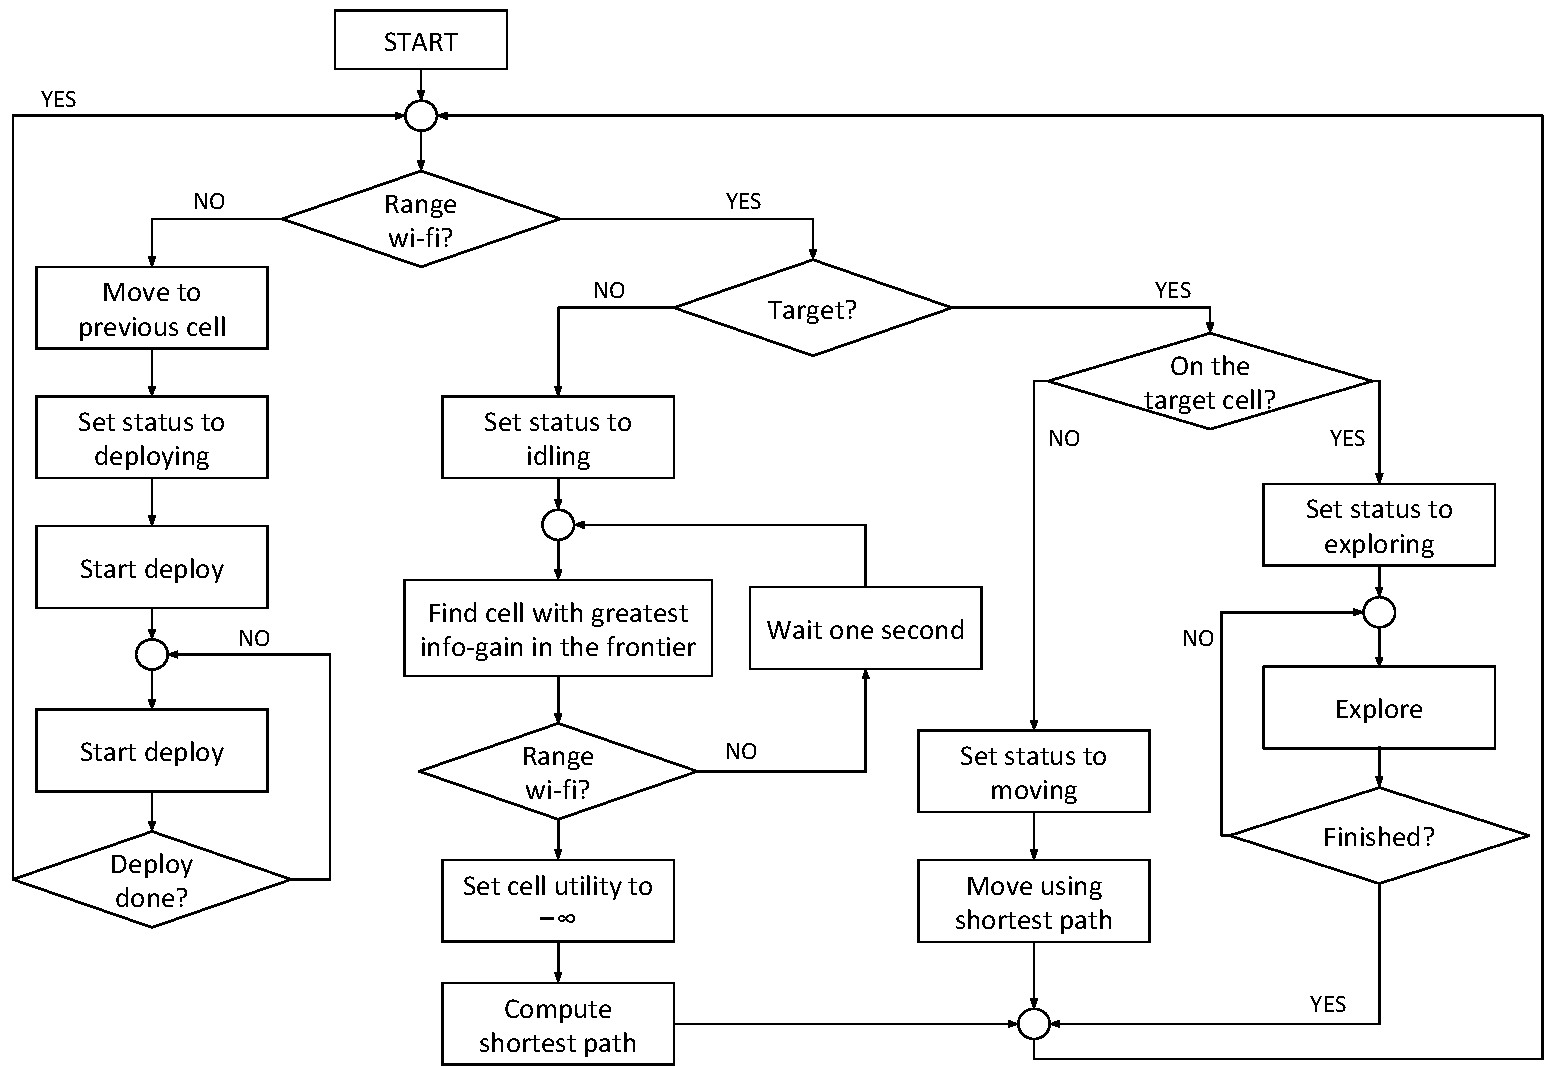
\includegraphics[width=1.0\linewidth]{images/Robot_workflow}
	\caption{Figura che rappresenta il processo decisionale che l'agente robot quando deve stabilire la sua prossima azione, tale processo si basa sullo stato interno del robot e sulla presenza (o assenza) di connessione con la rete \textit{mesh}; si noti, che quello appena descritto non avviene ad ogni step della simulazione ma solo quando lo stato interno dell'agente subisce dei cambiamenti.}
	\label{fig:robotworkflow}
\end{figure}
Per prima cosa, il robot valuta se è ancora all'interno della copertura \textit{wi-fi} poiché, per come è stato definito il metodo di comunicazione e coordinamento dei robot, risulta fondamentale che siano sempre in grado di comunicare tra loro.
Tale controllo risulta essere necessario farlo ogni volta che il robot, di fatto, si sposta di una cella perché è l'unico caso in cui si suppone che l'agente possa perdere la connessione uscendo dall'area coperta; per comodità e “pulizia” algoritmica viene anche effettuato nel caso in cuo il robot ha finito di esplorare una cella.
Quando il robot, muovendosi, esce dalla zona coperta, se ne accorge e allo \textit{step} successivo rientra immeditamente nella zona coperta iniziando il processo di rilascio del \textit{bean}: aggiorna il suo stato in fase di \textit{deploy}, iniziando poi il processo di rilascio il quale abbiamo supposto impieghi circa un 15 secondi (\textit{i.e.}, 15 \textit{step}) poiché il rilascio del ripetitore deve essere effettuato in un luogo e in modo sicuro.\\
Altrimenti, se il robot è in una zona coperta, la sua decisione viene determinata dal possedimento di una cella \textit{target}.
In particolare, se non possiede una cella obiettivo deve sceglierne una: per prima cosa, si mette in stato di \textit{idling}, ovvero lo stao rappresentante che il robot è fermo per calcolare il suo prossimo obiettivo oppure che non ha celle tra cui scegliere.
In seguito deve stabilire la cella “migliore” da esplorare; per far ciò, i robot sfruttano un concetto di \textit{information gain} (o \textit{info-gain}) \todo[inline]{qua mi sa che c'è da citare l'articolo dicendo cosa noi abbiamo cambiato rispetto a loro, puoi farlo te? Grazie DP} che è uno scalare che indica “quanta informazione può portare l'esplorazione di una cella”, ovvero più tale valore è alto più ad un agente conviene andare ad esplorare tale cella.
La Formula \ref{math:info-gain} è quella utilizzata dagli agenti per il calcolo dell'\textit{info-gain}, tale valore viene calcolato per ogni cella della frontiera.
\begin{equation}
	\label{math:info-gain}
	\textit{Information gain} = \rho+\mu-\alpha\omega
\end{equation}
In tale formula:
\begin{itemize}
	\item $\rho$ è la priorità della cella che risulta essere pari a zero tranne nei casi in cui la cella sia adiacente ad una cella in cui una vittima sia riuscita a segnalare la sua presenza;
	\item $\mu$ è l'utilità della cella;
	\item $\alpha$ è il parametro, già nominato in precedenza, che indica quanto il costo del percorso per raggiungere la cella d'interesse pesi nella scelta;
	\item $\omega$ è il costo, in termini di \textit{step} necessari per raggiungere la cella d'interesse.
\end{itemize}
Per il calcolo di $\omega$ per ogni cella della frontiera, viene computato il costo del cammino minimo sfruttando la rappresentazione interna del territorio che possegono (e condividono) i robot sotto forma di grafo; \textit{i.e.}, di fatto si calcolano insieme tutti i cammini minimi (e i loro costi) dalla cella in cui è presente il robot verso tutte le altre celle sfruttando l'algoritmo definito da Dijkstra.
Infine, verrà scelta la cella con \textit{info-gain} maggiore tra tutte le celle della frontiera, diventando così la cella \textit{target} dell'agente.
Se il robot è riuscito ad individuare la sua prossima cella obiettivo, imposta l'utilità di tale cella pari a $-\infty$ in modo che nessun altro agente scelga tale cella e poi \todo[inline]{perché la rimuoviamo in find best cell la cella dalal frotniera? non dovremmo rimuoverla quando il robot la esplora? per come abbiamo definito la frontiera quella cella è ancora in frotniera, come lo sistemiamo nella relazione? DP}.
Vi sono dei casi in cui è possibile che l'agente non riesca a stabilire il suo prossimo obiettivo perché non vi sono celle nella frontiera oppure perché tutte le celle hanno utilità pari a meno infinito e quindi stanno già venendo esplorate da un altro robot; in questi casi, i robot aspettano un secondo prima di riaggiornare la rappresentazione del territorio condivisa e poi cercano nuovamente una possibile cella.
% riduzione dell'utilità attorno alla cella scelta -> gamma
\todo[inline]{Anche questa riduzione non sarebbe da fare una volta che il robot arriva sulla cella e percepisce attorno? DP}
\todo[inline]]{Perché proprio diviso il radar radius? Puoi aggiungerlo te? Grazie DP}
% parametri
% metodo di comunicazione tra i robot
% metodologie di prioritizzazione
\todo[inline]{fallimenti parlarne altrove? DP}
\subsection{Ferito}
Questo agente rappresenta le persone ferite che sono disperse nell'area di interesse e necessitano di essere individuate e salvate, si noti che il loro salvataggio non fa parte di questo simulatore poiché le metodologie di salvataggio dipendono da troppi fattori che non possono venir considerati complessivamente in un simulatore (\textit{e.g.}, la loro possibilità di muoversi oppure se richiedono un intervento medico sul campo).
Il loro comportamento è stocastico ma basato su uno stato interno, di conseguenza tali agenti sono stati classificati come \textit{reflexive agent with internal state}, facendo riferimento alla classificazione proposta da Russell e Norvig \cite{russell2016}.
L'agente è molto semplice, possiede due attributi che lo descrivono: la posizione all'interno della griglia e lo stato interno; lo stato assume valore 0 nel momento in cui non è ancora stato trovato e 1 quando è stato trovato e quindi salvato successivamente.
Il suo comportamento, come detto, dipende dal suo stato interno, in particolare: 
\begin{itemize}
	\item finché tale agente non è stato individuato e la cella in cui si trova non è coperta dal \textit{wi-fi} non fa nulla;
	\item se si trova in una cella coperta e non è ancora stato individuato, ha una probabilità pari a $10^{-3}$ di segnalare la sua presenza collegandosi alla rete \textit{mesh}, tale probabilità risulta essere bassa perché bisogna considerare che ad ogni \textit{step} (un secondo di tempo d'orologio) della simulazione un ferito può segnalare la sua presenza ed inoltre non tutte le persone potrebbero aver accesso ad un telefono in una situazione critica;
	\item se è stato individuato da un robot o ha già segnalato la sua presenza, non fa altro che aspettare.
\end{itemize}
% Le due metodologie di prioritizzazione dei feriti le nasconderei sotto il cappuccio e ne parlerei nei robot DP
\chapter{Inferenza dei parametri $\alpha$ e $\gamma$ mediante un processo di ottimizzazione}
\label{chap:pso}
Nel seguete capitolo, si discuteranno brevemente le motivazioni che hanno portato a effettuare un tentativo di inferenza di parametri, il metodo di ottimizzazione utilizzato, i problemi di fattibilità che sono sorti e i risultati ottenuti.

\section{Motivazioni}
Come detto nel Capitolo \ref{chap:modeldesc}, $\alpha$ e $\gamma$ sono due parametri che vanno ad influire (direttamente o indirettamente) le celle scelte dagli agenti come loro obiettivi.
In particolare, $\alpha$ fa più o meno pesare il costo del cammino per raggiungere la cella di interesse: per valori elevati ci si aspetta che i robot scelgano delle celle con cammini poco costosi, per valori bassi ci si aspetta che i robot ignorino il costo del cammino prediligendo le celle con elevata utilità e priorità.
Al contempo, $\gamma$ ci si aspetta che influisca su quanto gli agenti tendano a tenersi distanti tra loro poiché influisce quanto l'utilità delle celle adiciacenti alla cella obiettivo di un robot diminuisce: valori bassi dovrebbero portare i robot a tenersi distanti tra loro, valori alti potrebbero portare i robot a muoversi in modo più coeso.\\
Si può facilmente intuire che la scelta della cella obiettivo è una componente fondamentale per permettere agli agenti robotici di esplorare in maniera efficiente (\textit{i.e.}, nel minor tempo possibile) il territorio; poiché tali scelte sono dettate da questi parametri, si vuole cercare una configurazione che permetta di esplorare nel minor tempo possibile il territorio.
In aggiunta, sono state effettuate delle considerazioni sui possibili costi monetari di tale sistema: la realizzazione di ogni robot e dei sistemi che utilizzano per percepire le celle circostanti sono costosi.
Quindi ci si è chiesto se davvero è meglio utilizzare il numero massimo di robot e permettergli di percepire il più distante possibile, oppure se vi sono delle soluzioni intermedie che permettono, comunque, l'esplorazione del territorio in modo efficiente con un utilizzo di un numero ridotto di robot.
Dato che si presenta un problema in cui bisogna stabilire dei valori di singoli parametri in cui il valore di alcuni può influire il valore ottimo di un altro, risulta necessario affrontare tale problema come un problema di ottimizzazione.
La funzione che si vuole minimizzare è la seguente:
\begin{equation}
\label{math:pso}
\textit{f} = \textit{S} + \frac{1}{n}\sum_{\textit{s} = 0}^{\textit{s} = \textit{S}}n_{\textit{is}}
\end{equation}
Dove:
\begin{itemize}
	\item \textit{S} è il numero totale di \textit{step} richiesti dalla simulazione;
	\item n è il numero di robot;
	\item $n_{\textit{is}}$ è il numero di robot in stato di \textit{idling} al \textit{s}-esimo \textit{step}.
\end{itemize}
In questo modo, si vuole minimizzare il tempo di epslorazione, ma si penalizza la funzione ogni volta che qualche robot è in stato di \textit{idling} perché non vi sono celle nella frontiera.\\
Poiché tale funzione, anche se espressa in termini matematici, non può essere risolta in modo analitico, si è deciso di utilizzare un processo di ottimizzazione meta-euristico: PSO (Particle Swarm Optimization), in particolare nella sua variante FST-PSO (Fuzzy Self-Tuning Particle Swarm Optimization) \cite{nobile2018} che viene descritta nella Sezione \ref{sec:fstpso}.

\section{PSO e FST-PSO}
\label{sec:fstpso}
PSO è una meta-euristica basata sull'intelligenza di sciame delle popolazioni, ispirata dagli stormi di uccelli e banchi di pesce. 
È particolarmente utile per problemi di ottimizzazione la cui soluzione può essere rappresentata come un vettore numerico \cite{Kennedy1995}. 
In PSO una popolazione (chiamata sciame) di \textit{N} soluzioni candidate (chiamate particelle) cooperano per identificare la soluzione ottima, rispetto ad una data funzione di fitness \textit{f}, muovendosi all'interno di un limitato spazio di ricerca \textit{M}-dimensionale, dove \textit{M} è la lunghezza del vettore di valori reali precedentemente citato. 
Ogni particella \textit{i} (\textit{i} = 1, \dots, \textit{N}) è caratterizzata da due vettori nello spazio di ricerca: la posizione, $x_i \in \mathbb{R}^\textit{M}$, e la velocità, $v_i \in \mathbb{R}^\textit{M}$. Le posizioni iniziali delle particelle sono selezionate casualmente mediante una distribuzione uniforme all'interno dello spazio di ricerca. 
La posizione e la velocità di ogni particella sono aggiornate, ad ogni iterazione della fase di ottimizzazione, basandosi su due attrattori: \begin{enumerate}
	\item la miglior posizione trovata dalla particella fino a quel momento ($\textbf{b}_i \in \mathbb{R}^\textit{M}$), la cui rispettiva costante globale, che ne bilancia l'effetto, prende il nome di fattore cognitivo ($c_{cog} \in \mathbb{R}_+$);
	\item la miglior posizione trovata, fino a quel momento, dallo sciame ($\textbf{g} \in \mathbb{R}^\textit{M}$), anche questa bilanciata da una costante globale denominata fattore sociale ($c_{soc} \in \mathbb{R}_+$).
\end{enumerate}
Fondamentalmente, il primo attrattore muove la particella verso la miglior soluzione che lei ha trovato sul proprio percorso, facendo in modo che si basi sulla propria esperienza personale; il secondo, invece, favorisce la collaborazione tra le particelle, muovendole verso la migliore soluzione trovata dallo sciame, o nelle vicinanze di essa. 
Dato che un movimento deterministico delle particelle può portarle a cadere in un minimo locale, ogni attrattore è moltiplicato per un numero casuale, estratto da una distribuzione uniforme nell'intervallo $[0, 1)$. 
Inoltre, l'aggiornamento della velocità è influenzato anche da un valore di inerzia (ovvero, si tiene in considerazione la direzione dove la particella si stava muovendo precedentemente a questa iterazione), $\textit{w} \in \mathbb{R}_+$. 
Formalmente, la velocità di ogni particella \textit{i} (\textit{i} = 1, \dots, \textit{N}) all'iterazione \textit{t} è data dalla seguente somma vettoriale:
\[\textbf{v}_i(t) = \textit{w}\cdot\textbf{v}_i(t - 1) + c_{soc}\cdot\textbf{R}_1\bigcirc(\textbf{x}_i(t - 1) - \textbf{g}(t - 1)) + c_{cog}\cdot\textbf{R}_2\bigcirc(\textbf{x}_i(t - 1) - \textbf{b}_i(t - 1)),\]
dove $\bigcirc$ indica un operatore di moltiplicazione tra due vettori elemento per elemento (\textit{component-wise}) e $\textbf{R}_1$ e $\textbf{R}_2$ sono due vettori di numeri casuali associati, rispettivamente, a fattore sociale e al fattore cognitivo. Di conseguenza, la posizione della particella è determinata come: 
\[\textbf{x}_i(t) = \textbf{x}_i(t - 1) + \textbf{v}_i(t).\] 
Si vuole sottolineare che, in PSO i valori del peso dell'inerzia, del fattore cognitivo e di quello sociale (\textit{w}, $c_{cog}$, $c_{soc}$) sono indipendenti dall'iterazione che si sta effettuando e sono comuni a tutto lo sciame, ovvero sono dei valori costanti durante tutta la simulazione. Per stabilire “quanto una soluzione è buona” si utilizza la funzione di fitness \textit{f} che ha lo scopo di stabilire i valori di $\textbf{b}_i$ e di \textbf{g}.

Per come è stata descritta fin'ora, la tecnica potrebbe portare le particelle al di fuori dello spazio delle soluzioni accettabili. 
Per evitare questo problema, in PSO lo spazio di ricerca è limitato, basandosi su conoscenze di dominio del problema, e queste condizioni di confine sono applicate a tutte le particelle che raggiungono tali limiti.
Si evidenzia che i confini dello spazio di ricerca sono dipendenti dal problema e, quindi, non possono essere determinati a priori con strategie automatiche. 
Le condizioni al confine usate da PSO (e riutilizzate in FST-PSO) seguono una \textit{damping strategy}, una strategia consistente nel “far rimbalzare” le particelle che escono dai confini modificando la loro velocità rispetto alla dimensione di cui è stato oltrepassato il limite. 
Alla particella di interesse viene impostata la direzione come l'opposto della direzione che l'ha portata ad uscire, moltiplicata per un valore estratto casualmente da una distribuzione uniforme nell'intervallo $[0, 1)$. 
PSO presenta un altro problema riguardante la velocità delle particelle; essa infatti può divergere durante la simulazione. 
Per impedire ciò, è presente un valore di velocità massima $\textit{v}_{max_m} \in \mathbb{R}_+$ (dove tale velocità è riferita all'\textit{m}-esima dimensione dello spazio di ricerca, $\textit{m} = 1, \dots, \textit{M}$) che non può essere superato dalle particelle. Nel caso in cui questo limite venisse infranto, la velocità della particella sarebbe riportata a tale valore. 
È inoltre possibile, teoricamente, impostare una velocità minima $\textit{v}_{min_m} \in \mathbb{R}_+$ (anche in questo caso la velocità minima è riferita ad ogni direzione) a cui possono viaggiare le particelle, in modo da migliorare le capacità esplorative dello sciame. Tale costante, però, non è presente nell'implementazione di PSO standard.

Tuttavia, in PSO, i valori delle costanti descritte fin'ora (\textit{N}, $c_{cog}$, $c_{soc}$, \textit{w}, il vettore delle velocità minime $\textbf{v}_{min}$, se presente, e il vettore delle velocità massime $\textbf{v}_{max}$) devono essere impostati dall'utente. 
Il problema che si pone è che il valore di queste costanti può influenzare significativamente il processo di ottimizzazione, in quanto influiscono sia sulla velocità di convergenza della tecnica sia sulla qualità della soluzione ottima. 
Questo implica che l'utente sia obbligato a fare più iterazioni del processo di ottimizzazione, cercando le giuste configurazioni di costanti per ottenere dei buoni risultati; ciò può richiedere un grande dispendio in termini temporali e prestazionali. 
Inoltre, spesso buone conoscenze sul dominio applicativo su cui si sta effettuando il processo di ottimizzazione, possono influenzare il numero di iterazioni richiesto, poiché permettono di impostare tali costanti più facilmente.

Per i motivi sopracitati, è stato introdotto e si è deciso di usare FST-PSO, alla cui base vi è la logica sopra descritta. 
Tale processo estende un già presente sistema di ottimizzazione, basato anch'esso sulla logica Fuzzy, che prende il nome di PPSO (Proactive Particles in Swarm Optimization) \cite{nobile2015}. 
La particolarità di PPSO è che la velocità e la posizione della particella sono aggiornate in base a valori delle costanti individuali per quella particella, l'inerzia e i fattori sociali e cognitivi erano associati rispettivamente a diverse variabili della logica Fuzzy indipendenti tra ogni particella della popolazione (ognuna possedeva le sue variabili). 
Inoltre, in PPSO le velocità minime e massime rispetto ad ogni dimensione dello spazio di ricerca erano comuni tra tutte le particelle. 
Al contrario, FST-PSO incorpora anche queste due costanti “all'interno” delle particelle, in modo tale che ogni particella abbia associate a sè le seguenti costanti (i cui valori sono indipendenti dai valori delle stesse delle altre particelle): \begin{itemize}
	\item $c\_{cog}$;
	\item $c\_{soc}$;
	\item \textit{w};
	\item $\textbf{v}_{min}$;
	\item $\textbf{v}_{min}$.
\end{itemize}
I valori di queste 5 costanti sono modificati durante il processo di ottimizzazione basandosi sui valori di uscita determinati da alcune regole Fuzzy. 
Inoltre, il numero di particelle della popolazione, che dev'essere utilizzato per il processo di ottimizzazione, è stabilito dalla seguente euristica: $\textit{N} = \lfloor10 + 2\sqrt{\textit{M}}\rfloor$.
Quindi il numero di particelle dipende dal numero delle dimensioni dello spazio di ricerca \textit{M}.\\
Per quanto riguarda questo lavoro, è stato sfruttato FST-PSO perché permette all'utente evitare la scelta di tutte le costanti sopra descritte, i cui valori sono impostati automaticamente seguendo delle regole di logica Fuzzy, e sono relative alla singola particella.

\section{Problemi riscontrati e risultati}
\label{sec:psoResults}
Dato che lo scopo, semplificando, è quello di minimizzare una funzione e quindi eseguire tante simulazioni con parametri diversi tra loro, al fine di scoprire quale configurazione permette di ottenere il minimo valore di \textit{fitness}, ci si trova a dover affrontare delle problematiche legate ai tempi richiesti della simulazione.
Originariamente, si era supposto che l'area da esplorare fosse di 1 $Km^2$ ovvero di circa 333$\times$333 celle; da un punto di vista pratico, tali simulazioni richiedono un elevato lasso di tempo, poiché griglie così grandi vanno ad ingrandire significativamente il grafo di visione sfruttato dai robot e richiedono un numero maggiore di robot.
Di conseguenza, l'operazione di calcolo dei cammini minimi diventa computazionalmente onerosa, richiedendo tempi sempre più elevati nella pratica (diverse ore per la singola simulazione).
Poiché per un processo di ottimizzazione (per come è stato definito PSO) richiede un numero di simulazioni nell'ordine delle centinaia, non è risultato possibile effettuare tutto il processo di ottimizzazione con mappe di tali dimensioni (il singolo processo avrebbe richiesto settimane).
Si è quindi deciso di ridurre la scala del problema andando ad analizzare griglie con dimensioni di 30$\times$30 celle e 3 feriti, scalando proporzionalmente anche il raggio di copertura del singolo ripetitore \textit{wifi}.
In questo modo, è stato possibile effettuare una singola volta (poiché effettuarlo più volte avrebbe richiesto comunque troppo tempo) il processo di ottimizzazione, considerando validi i risultati inferiti sia in termini del numero di robot da utilizzare (anche questi in proporzione) sia in termini di valori di $\alpha$ e $\gamma$, che ci si aspetta non debbano modificarsi al variare delle dimensioni della mappa, in quanto influiscono sulle scelte “locali” ed esse non vengono influenzate in alcun modo dalla dimensione della mappa o dal numero di robot.
Per queste motivazioni, abbiamo considerato estendibili i risultati ottenuti a mappe di dimensioni maggiori.\\
Gli intervalli di valori assumibili da tali parametri che hanno determinato lo spazio di ricerca sono:
\begin{itemize}
	\item $\left[1, 6\right]$ per il numero di robot da dispiegare, il valore è arrotondato all'intero più vicino;
	\item $\left[1, 10\right]$ per il raggio di percezione del radar misurato in numero di celle, anche in questo caso il valore è arrotondato all'intero più vicino;
	\item $\left[0.001, 10\right]$ per il valore di $\alpha$;
	\item $\left[0, 1\right]$ per il valore di $\gamma$.
\end{itemize}
Infine, il numero di iterazioni effettuate dal processo è pari a 50.
Poiché l'esecuzione singolo processo di ottimizzazione in queste condizioni richiede diversi giorni, è stato effettuato una sola volta in modo da poter poi effettuare altri studi qualitativi. 
Nonostante sia stato effettuato una sola volta, possiamo considerare i risultati prodotti abbastanza attendibili, in quanto l'algoritmo ha presentato convergenza verso la soluzione ottima già dalle primissime iterazioni, e non è riuscito a trovare configurazioni che migliorassero significativamente il risultato (si faccia riferimento all'Appendice \ref{apx:pso}).
Per garantirci di non essere incappati in un minimo locale, abbiamo valutato il valore della funzione di fitness rispetto alla difficoltà complessiva di esplorazione della mappa e i due valori sono concordi tra loro; possiamo quindi affermare, con un buon margine di sicurezza, che i risultati prodotti siano quelli effettivamente ottimi.
In particolare, $\alpha$ deve essere pari a 8.233, ovvero un valore molto alto che va a far pesare significativamente il costo del cammino; questo implica che se si vuole esplorare in maniera efficiente bisogna ridurre il più possibile i tempi di spostamento.
Per quanto concerne $\gamma$, il valore ottimo è pari a 0.65; ciò indica che vi sia una tendenza a tenere gli agenti relativamente coesi, ma al tempo stesso si vuole evitare che preferiscano percorsi costosi solo perché una cella presenta un valore maggiore di utilità.
Valutando insieme i due parametri, si può intuire come la soluzione deve essere quella di non ridurre in maniera significativa l'utilità delle celle in modo che agenti vicini possano continuare a muoversi appaiati se gli conviene in termini di percorso ottimo, ma allo stesso tempo far pesare significativamente il costo del cammino in modo da evitare che agenti abbiano la tendenza a esplorare celle in aree molto distanti dalla loro posizione.
Per quanto riguarda il numero di robot, il processo propone di utilizzarne il massimo; questo risulta ragionevole poiché più robot si utilizzano, più velocemente si esplora. La nota interessante è che il numero di robot massimo non penalizza la funzione di \textit{fitness} tanto da portare il processo di ottimizzazione a utilizzare un numero inferiore di robot; su questo punto si discuterà nuovamente nella Sotto-sezione \ref{subsec:nrobots}.
Infine, il raggio di percezione dei robot è pari a 6 celle; tale risultato è interessante, poiché significa che un aumento di tale parametro non implicherebbe \textit{performance} migliori da parte del sistema.
\chapter{Risultati}
\label{chap:results}
come $\alpha$ influisce nel costo del cammino scelto durante i vari \textit{step} della simulazione e come varia il costo medio durante tutta la simulazione al variare del parametro\\
come il variare di $\gamma$ influisce la distanza (euclidea) tra i robot, sia con un valore di $\alpha$ elevato sia con uno basso\\
\\
Macroscopiche:\\
mappa fissa, come il numero di robot influisce la quantità di ripetitori rilasciati\\
Come le dimensioni della mappa influiscono il numero di bean rilasciati (raggio pari a 3)\\
Come la difficoltà totale influisce il numero di step richiesto\\
Mappa fissa(?), come numero di robot influisce fitness\\
\\
Il numero dei robot in uno stato al durante l'esplorazione (robot\_status)\\
\section{Analisi macroscopiche}
\label{sec:results-macro}
Le seguenti analisi hanno lo scopo di rilevare delle possibli relazioni di come alcune caratterisitche (o parametri) del sistema ne possano influire degli altri.
Per effettuare tali analisi, poiché si tratta di un sistema complesso, è stato necessario effettuare un insieme di simulazioni in modo tale da raccogliere i dati che derivano dal comportamento emergente.
Poihé in questa Sezione si presentano analisi differenti tra loro, ogni volta verrà descritta la metodologia utilizzata per la raccolta dati.
Si tenga presente, che il metodo di prioritizzazione delle celle dovuto alla segnalazione di feriti segue la strategia che attribuisce una bassa priorità.\\
Gli studi effettuati sono i seguenti:\begin{itemize}
	\item come il numero dei robot influisce il numero di ripetitori rilasciati e come fa variare il valore di fitness;
	\item come la dimensione della mappa influisce il numero di ripetitori che devono venir rilasciati dagli agenti;
	\item come la difficoltà totale della mappa influenza il numero di step richiesto per completare l'esplorazione.
\end{itemize}
\subsection{Studio sul numero di robot}
\label{subsec:nrobots}
Come già detto, sul variare del numero dei robot sono state effettuate due analisi riguardo due aspetti diversi del sistema.
In entrambi i casi, però, la metodologia di raccolta dati è stata analoga: per tutte le simulazioni effettuate si è mantenuta la stessa mappa \todo{siamo sicuri che anche per la fitness la mappa fosse fissa? DP}di dimensioni 30$\times$30 di cui ci si è garantiti che non presentasse al suo interno casi patologici (\textit{e.g.}, zone inesplorabili poiché irraggiungibli).
Inoltre, i valori di $\alpha$, $\gamma$ e per il raggio dei sensori sono stati utilizzati quelli inferiti dal processo di ottimizzazione, descritto nel Capitolo \ref{chap:pso}, il \textit{range} del ripetitore è stato mantenuto pari a 3 celle in modo da avere risultati scalati correttamente rispetto alle dimensioni che erano state considerate originariamente (mappe 333$\times$333); infine, per ogni valore del numero di robot sono state effettuate 10 simulazioni e i feriti potevano segnalare la loro presenza \todo{confermi? DP}.

Per quanto concerne \margin{Numero di robot \textit{vs} ripetitori rilasciati}il numero di ripetitori rilasciati, come mostrato in Figura \ref{fig:robotsbeans} tale numero aumenta all'aumentare dei robot impiegati nonostante le dimensioni della mappa rimangono costanti.
Tale comportamento può essere considerato ragionevole perché all'aumentare del numero dei robot aumentano i casi in cui due agenti escono contemporaneamente dalla zona coperta e quindi rilasciano due ripetitori la cui area coperta di uno dei due sarebbe bastata per coprire anche parzialmente l'area dell'altro.
Di fatto, i robot non hanno alcun meccanismo di coordinamento per la creazione della rete, ognuna pensa a sé e quindi all'aumentare del numero di robot aumentano i casi in cui due robot rilasciano due ripetitori vicini tra loro non ottimizzando l'utilizzo del singolo ripetitore, portando quindi a molte porzioni di territorio coperte da più di un singolo ripetitore.
Si fa presente, che tale numero non è distorto dal fatto che ogni singolo robot rilascia un ripetitore appena viene disposto sul campo, poiché i robot rilasciano il ripetitore solo se in quella cella non vi è già presente un ripetitore.
\begin{figure}
	\centering
	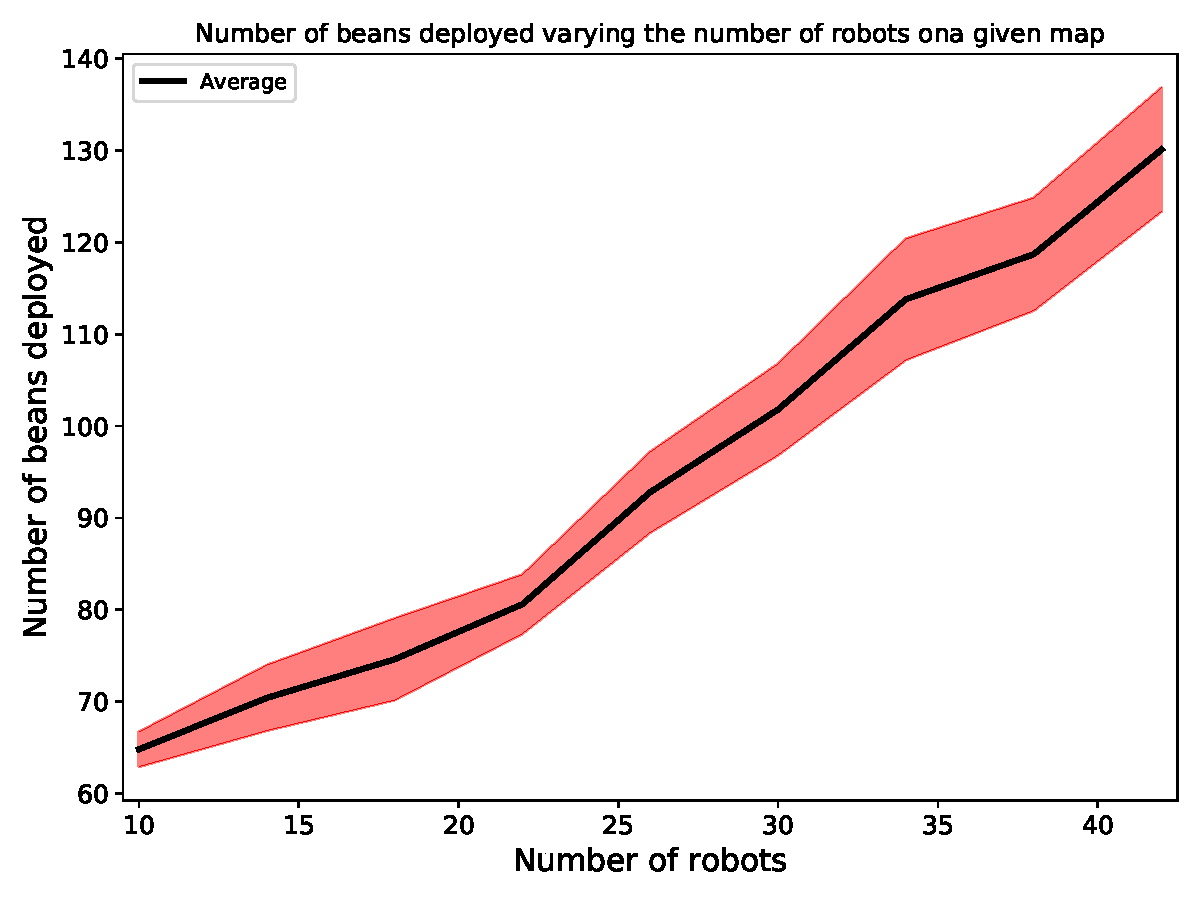
\includegraphics[width=0.9\linewidth]{images/macro_results/robots_beans}
	\caption{In Figura è rappresentato come il numero di robot influisce il numero di ripetitori rilasciati nel territorio. Sull'asse delle \textit{x} è presente il numero di robot e sull'asse delle \textit{y} il numero di ripetitori disposti. Sono state effettuate 10 simulazioni per ogni valore di numero di robot, in nero è presente la media del numero di ripetitori rilasciati e l'area rossa indica la deviazione standard.}
	\label{fig:robotsbeans}
\end{figure}

Invece, rispetto alla seconda analisi effettuata, si evidenzia che il valore di fitness è quello definito nella Formula \ref{math:pso}.
Per quanto riguarda i risultati ottenuti mostrati in Figura \ref{fig:fitness} si nota come con un numero di robot basso la fitness diminuisce velocemente perché il tempo di esplorazione del territorio diminuisce significativamente; al contrario, con un numero elevato di agenti il valore di fitness diminuisce molto più lentamente perché il tempo di esplorazione non subisce diminuzioni significative e nel mentre vi è un numero sempre maggiore di robot in stato di \textit{idling} mentre ci si approccia al termine dell'esplorazione.
Si fa presente, che i valori rappresentati dai segni tondi in rosso sono il valore medio di fitness che si ha ottenuto con tale numero di robot, invece, le barre nere (poco visibili) indicano la variazione data dalla deviazione standard; il fatto che spesso non si vedano è dato da fatto che la deviazione standard è molto bassa.
Considerando il grafico mostrato e concentrandosi sull'intervallo tra i 51 e 76 robot, ci si pone una domanda aperta a cui servirebbero analisi di costi successive e non fattibili nei termini di questo lavoro: “vale la pena utilizzare 10, 15 o addirituttra 25 robot in più se il valore di fitness e il tempo di esplorazione diminuiscono poco significativamente?”.\\
Pensiamo che per rispondere a questa domanda (escludendo i dibattiti etici a riguardo) sia necessario fare delle analisi tenendo conto il costo di realizzazione dei robot e di quanti robot si hanno a disposizione nella pratica e se sia necessario intervenire su un solo quartiere o più quartieri.
\begin{figure}
	\centering
	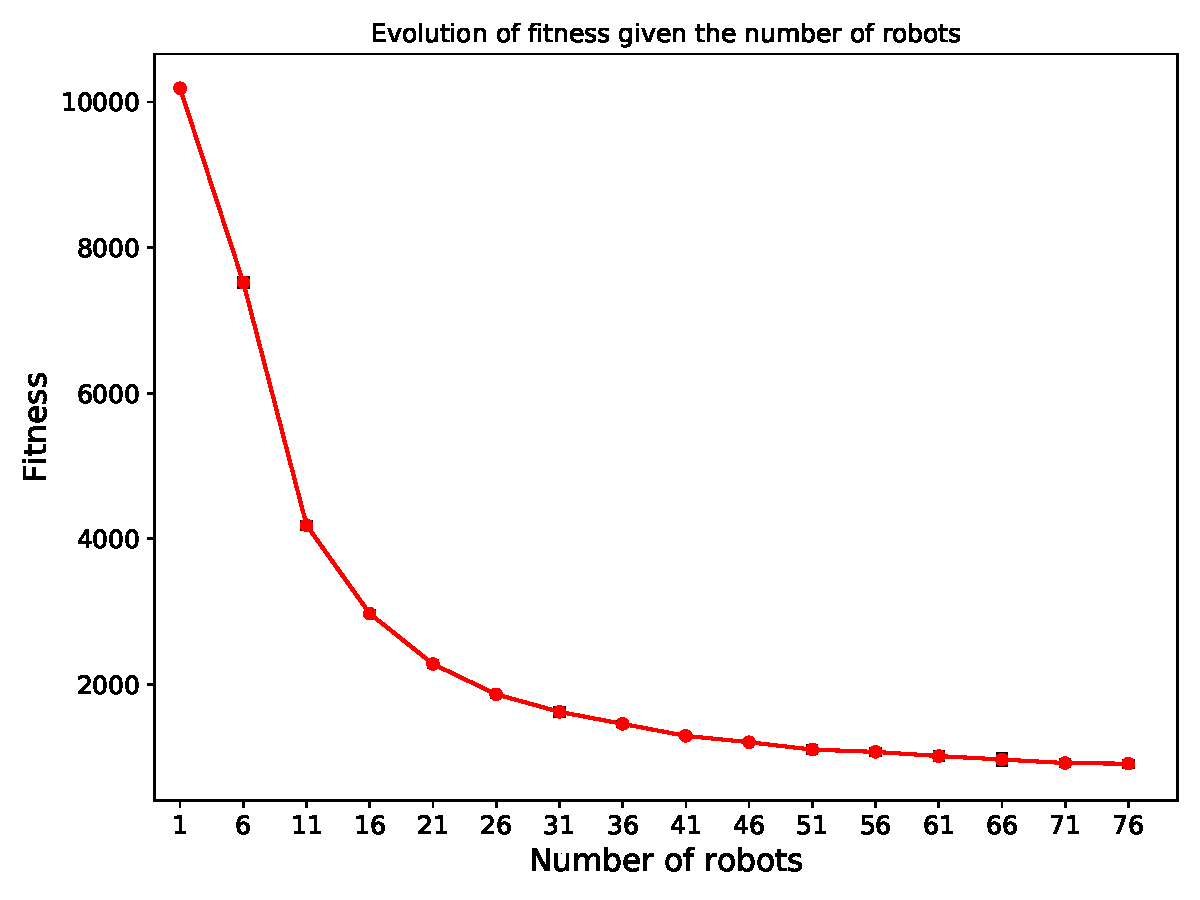
\includegraphics[width=0.9\linewidth]{images/macro_results/fitness}
	\caption{Sull'asse delle \textit{x} è indicato il numero di robot, su quello delle \textit{y} il valore di fitness. Poiché per ogni valore sono state effettuate 10 simulazioni, i valori rappresentati sono la media invece in nero sono le barre di errore date dalla deviazione standard, risultano poco visibili poiché i valori di deviazione standard sono molto piccoli rispetto alle scale del grafico.}
	\label{fig:fitness}
\end{figure}

\subsection{Dimensioni della mappa \textit{vs} numero di ripetitori rilasciati}
\todo[inline]{Non ho trovato il csv che ha generato tale immaigne, quindi controlla tutto quello che ho detto, soprattutto che abbiamo fatto 10 simulazioni per ogni dimensioni. Devi esserne certo, non andare a memroia DP}
Per la produzione di questa analisi, sono state effettuate 10 simulazioni per ogni dimensione della mappa considerata, le mappe sono state generate casualmente ad ogni simulazione, i parametri sono stati utilizzati quelli inferiti dal processo di ottimizzazione (si veda il Capitolo \ref{chap:pso}), il raggio dei ripetitori pari a 3 celle e i feriti erano in grado di poter segnalare la loro presenza. \todo{il numero di robot quant'era? DP}.
I risultati mostrati in Figura \ref{fig:beans}, dove la linea nera è la media e l'area in rosso rappresenta la deviazione standard, mostrano che all'aumentare della dimensione del territorio il numero di ripetitori aumenta (come ragionevole) in maniera assimilabile qualitativamente ad una crescita quadratica.
Questo risultato è più che ragionevole considerando che l'aumentare della dimensione del lato dalla mappa fa aumentare la dimensione di un quadrato portando quindi ad una crescita quadratica delle dimensioni che si riflette coerentemente nel numero di ripetitori necessari.
È interessante notare, aggregando questo dato a quello presentato nella Sotto-sezione \ref{subsec:nrobots}, che l'aumento del numero di ripetitori disposti viene influenzato maggiormente dal numero di agenti impiegati e dal fatto che non si coordinano tra loro rispetto alle dimensioni effettive della mappa che implica una crescita che è intrinseca con l'aumento delle dimensioni della mappa.
\begin{figure}
	\centering
	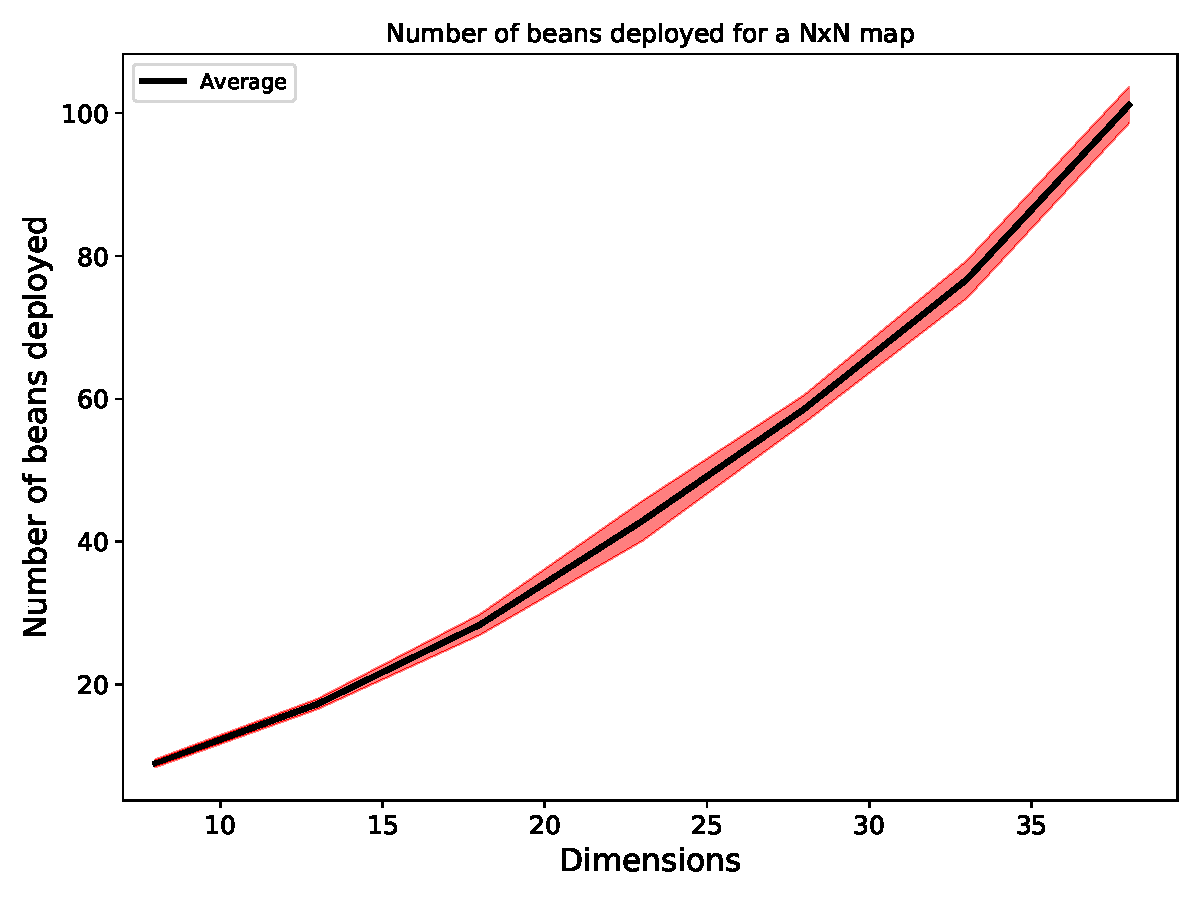
\includegraphics[width=0.9\linewidth]{images/macro_results/beans}
	\caption{Figura che rappresenta come all'aumentare delle dimensioni del territorio (sull'asse delle \textit{x} è rappresentata la dimensione del lato della mappa) aumenta il numero di ripetitori (sull'asse delle \textit{y}) necessari per coprire tutta l'area. In nero è rappresentato il valore medio, mentre in rosso la deviazione standard.}
	\label{fig:beans}
\end{figure}

\subsection{Difficoltà della mappa \textit{vs} tempo richiesto}
\todo[inline]{Mi confermi che i dati sono quelli nel csv robot\_step\_difficulty.csv? DP}
Per tale studio, sono state effettuate un totale di 7 simulazioni in cui si è fatto aumentare la dimensione della mappa, e con esso in maniera proporzionale il numero di robot impiegati, in modo tale da far aumentare la difficoltà complessiva; per difficoltà complessiva si intende la somma delle difficoltà di ogni singola cella.
Le mappe sono state generate casualmente e si è deciso di non effettuare più simulazioni per ogni difficoltà per non complicare inutilmente il grafico e il processo di generazione dati in aggiunta a tutto il tempo richiesto da tali simulazioni; inoltre, i risultati ottenuti da queste poche simulazioni sono stati considerati soddisfacenti per delle analisi di massima.\todo{sicuramente da sistemare. DP}
Siamo anche convinti che effettuare analisi di fino su queste quantità richiederebbero di prendere in considerazione un numero evelato di fattori e i risultati prodotti potrebbero non risultare altamente interessanti, soprattutto contando che nella pratica ogni situazione sarà unica e poco prevedibile a priori.\\
Per quanto riguarda i risultati riportati in Figura \ref{fig:difficulty} , si nota che anche in questo caso l'aumento di \textit{step} richiesti per completare l'esplorazione non è lineare rispetto alla difficoltà ma presenta piuttosto un andamento più assimilabile a quello di un logaritmo.
In aggiunta a tale prima analisi non è possibile trarre altre conclusioni significative, servirebbero molte più simulazioni e sarebbe necessario definire una strategia complicata per poter tenere in considerazioni più fattori per proporre un'analisi approfondita di tale relazione.
\begin{figure}
	\centering
	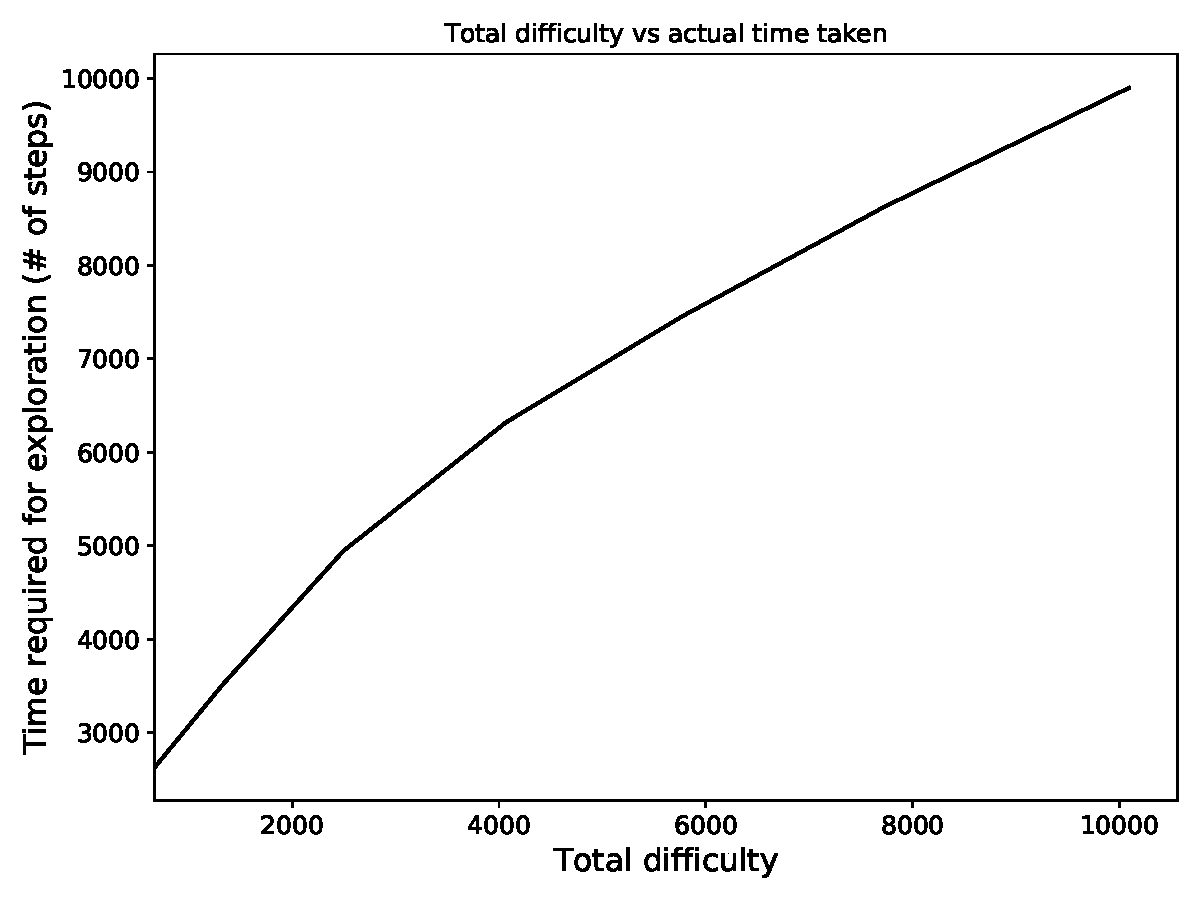
\includegraphics[width=0.9\linewidth]{images/macro_results/difficulty}
	\caption{Sull'asse delle \textit{x} è presente la difficoltà complessiva di esplorazione della mappa e sull'asse delle \textit{y} il numero di \textit{step} effettuati per completare l'esplorazione.}
	\label{fig:difficulty}
\end{figure}

\section{Analisi del parametro $\alpha$}
\label{sec:alpha}
Nelle seguenti analisi si è voluto studiare come al variare del parametro $\alpha$ variasse la scelta delle celle obiettivo da parte dei robot (si ricorda la strategia di scelta della cella descritto nella Sotto-sezione \ref{sub:robots} e della Formula \ref{math:info-gain}), ovvero come il peso introdotto da $\alpha$ fa variare l'importanza che gli agenti danno alla scelta dei cammini.
Come già detto, ci si aspetta che per valori di $\alpha$ elevati si scelgano celle il cui cammino per raggiungerle abbia un costo basso, e per valori di $\alpha$ bassi i robot scelgano principalmente in base all'utilità (e priorità) della cella.\\

In questa parte di lavoro, sono state effettuate due tipi di analisi: in primo luogo, si sono studiati i costi dei cammini scelti durante tutta la durata della simulazione aggregando i risultati di varie simulazioni con lo stesso valore di $\alpha$; in seguito, si è scesi più nel dettaglio andando a valutare come i costi variano all'evolvere del tempo (in termini di \textit{step}) per ogni valore di $\alpha$ studiato in precedenza.
Tutte le simulazioni effettuate per queste analisi sono state eseguite nel seguente modo:
\begin{itemize}
	\item la dimensione della mappa è 30$\times$30 celle con 6 robot disposti all'esplorazione;
	\item il valore di $\gamma$ pari a 0.65 (inferito dal processo di ottimizzazione);
	\item il raggio di percezione pari a 6 celle (anche questo inferito dal processo di ottimizzazione);
	\item il raggio dei ripetitori \textit{wi-fi} pari a 3 celle, in modo da tenerlo proporzionale con la riduzione in scala della mappa rispetto alle dimensioni iniziali che si erano pensate.
\end{itemize}
Infine, per ogni valore di $\alpha$ sono state effettuate 10 simulazioni su mappe scelte casualmente da un insieme di 5 mappe pregenerate in modo \textit{randomico}, le quali non presentano casi patologici.

I risultati delle analisi aggregate sono mostrate in Figura \ref{fig:alphaVar}, in particolare nella Figura \ref{sfig:alphaVarAll} viene mostrata la media dei valori medi (in nero) e relative medie delle deviazioni standard (in rosso) dei costi dei cammini scelti al variare di $\alpha$, la linea tratteggiata rappresenta il valore massimo di deviazione standard dei costi che si è rilevato durante una simulazione.
Poiché i valori di $\alpha$ sono stati studiati con ordini di grandezza differenti (da $10^{-4}$ a $10$), è stato necessario produrre un altro grafico che si concentrasse solo sui valori di $\alpha$ molto piccoli; tale grafico viene mostrato in Figura \ref{sfig:alphaVar0.005}, dove la rappresentazione grafica segue la semantica utilizzata per il grafico precedente.
Dai grafici si nota che per valori relativamente alti di $\alpha$ il costo medio rimane pressoché costante, questo perché nel momento in cui $\alpha$ è sufficiente a far pesare, anche solo in piccola parte, il costo del cammino nel calcolo dell'\textit{info-gain}, le celle in prossimità dell'agente saranno quelle che tipicamente possiedono un valore di \textit{info-gain} maggiore e verranno quindi preferite dall'agente, portando così a costi di spostamento ridotti.
Al contempo, si può apprezzare come all'aumentare del parametro, nonsotante la media rimanga invariata, la deviazione standard e relativo massimo diminuscano, evidenziando che i robot tenderanno sempre più a preferire le celle più economiche da raggiungere a discapito di una loro utilità e priorità bassa.
Si può dedurre che valori di $\alpha$ troppo elevati rendano inutili le politiche di prioritizzazione delle celle e le strategie di gestione delle utilità, poiché gli agenti preferiranno sempre e solo la cella più economica da raggiungere, ignorando gli altri due parametri.
Infine, in Figura \ref{sfig:alphaVar0.005} si può notare come per un valore di $\alpha$ pari a zero il costo venga completamente ignorato (come ci si aspetta) e quindi le celle scelte dipendono unicamente dalla loro utilità e priorità, causando quindi lo spostamento degli agenti per il territorio, cercando semplicemente la cella con utilità e priorità maggiore. Questo porta ad un drastico aumento del numero di \textit{step} necessari a completare la simulazione, in quanto la maggior parte del tempo è impiegato per lo spostamento dei robot.
\begin{figure}
	\subfloat[Media dei costi dei cammini scelti da parte degli agenti durante un insieme di simulazioni con un determinato valore di $\alpha$, relative deviazioni standard e massima deviazione standard presente in una simulazione. In questa figura sono rappresentati i dati relativi a tutti i valori del parametro analizzati.\label{sfig:alphaVarAll}]{
		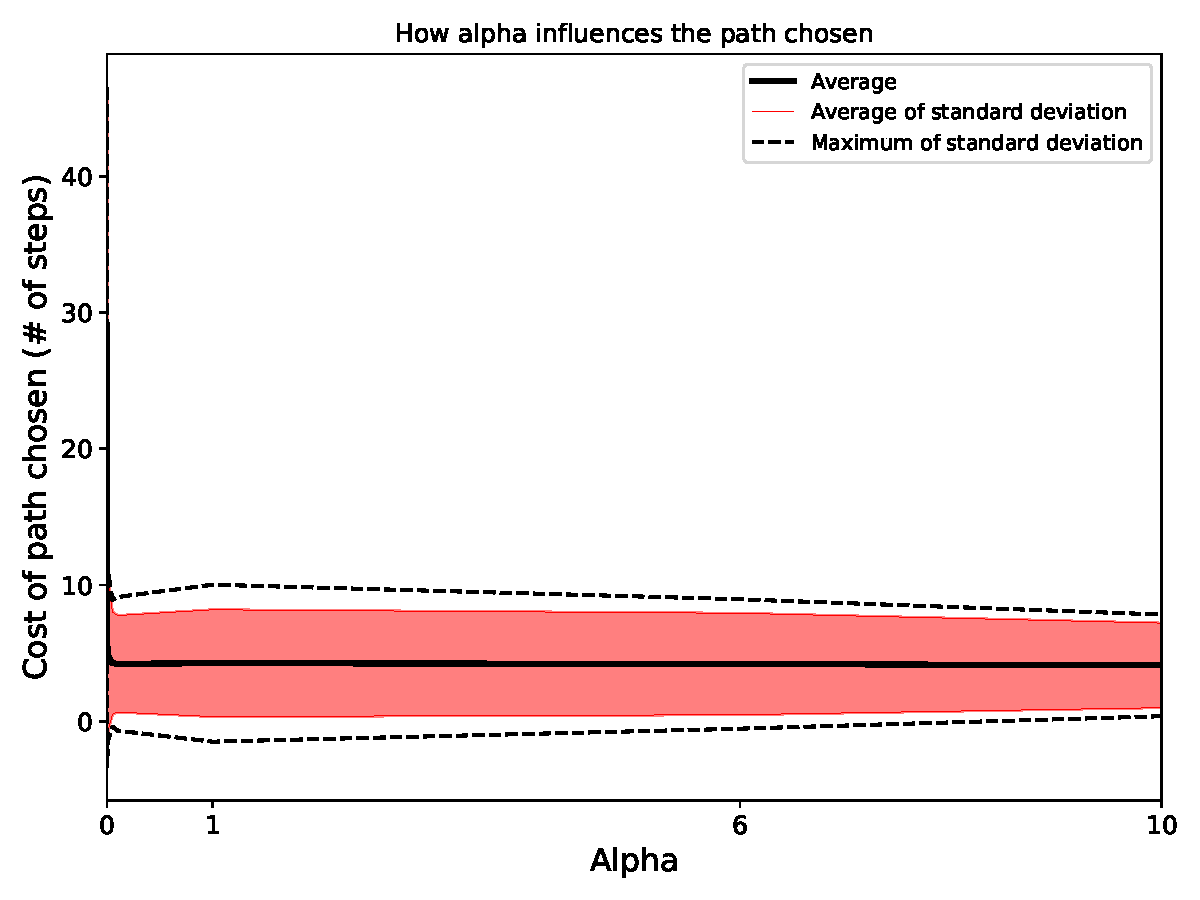
\includegraphics[width=.47\linewidth]{images/alpha_results/variation_all}
	}
	\hfill
	\subfloat[Media dei costi dei cammini scelti da parte degli agenti durante un insieme di simulazioni con un determinato valore di $\alpha$, relative deviazioni standard e massima deviazione standard presente in una simulazione. In questa figura sono rappresentati i dati relativi ai valori del parametro pari a 0, $10^{-4}$, $5\times10^{-4}$, $10^{-3}$, $5\times10^{-3}$.\label{sfig:alphaVar0.005}]{
		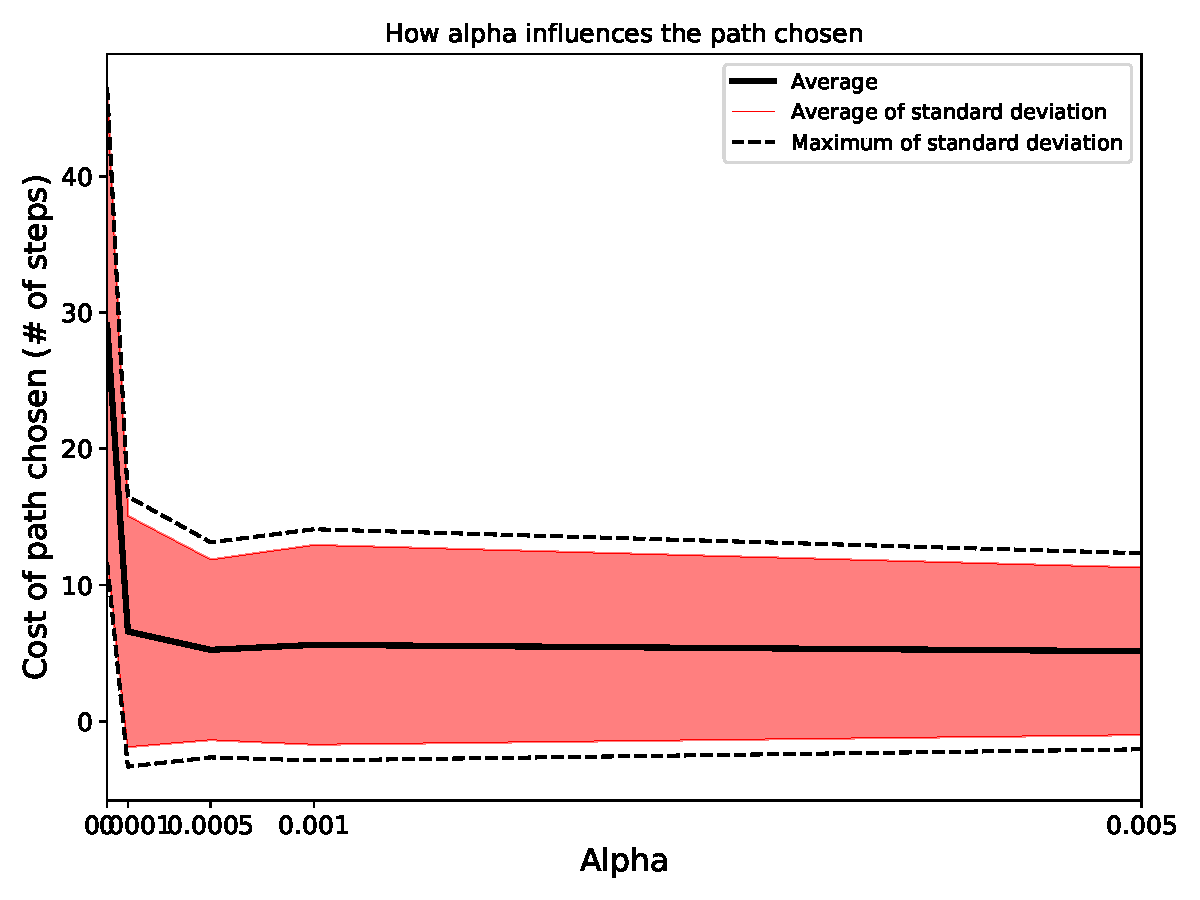
\includegraphics[width=.47\linewidth]{images/alpha_results/variation_0_005}
	}
	\caption{Per entrambi i grafici, in nero è rappresentata la media delle medie dei costi durante le singole simulazioni effettuate con un determinato valore di $\alpha$, in rosso si rappresenta la media delle deviazioni standard calcolate per ogni simulazione ed infine la riga tratteggiata indica il massimo delle deviazioni standard delle simulazioni per il relativo valore di $\alpha$.}
	\label{fig:alphaVar}
\end{figure}

Poiché le analisi precedentemente introdotte aggregano i dati in modo sostanziale, si è deciso di analizzare più nello specifico come $\alpha$ influisse nella scelta dei cammini durante la simulazione, in particolare per ogni valore di $\alpha$ preso in considerazione nella parte precedente si è valutato per ogni \textit{step} della simulazione i costi dei cammini scelti dagli agenti.
Si sono considerati solo gli \textit{step} in cui almeno un robot ha effettuato la scelta della cella \textit{target} e se più robot hanno effettuato una scelta nello stesso \textit{step}, si è considerata la media di essi; tale studio è stato effettuato aggregando le varie simulazioni per lo stesso valore del parametro. 
Con il termine aggregazione intendiamo in questo caso andare a valutare contemporaneamente per ogni \textit{step} cosa è successo durante le varie simulazioni.
I grafici per alcuni valori di $\alpha$ che sono stati ritenuti significativi sono stati riportati in Figura \ref{fig:alphaOverTime}, invece, mentre per i grafici dei restanti valori si rimanda all'Appendice \ref{apx:alpha}. Si noti che, per rendere i grafici leggibili, sono stati accorpati i valori dei costi per intervalli di 100 \textit{step} l'uno; di conseguenza viene rappresentata la media (evidenziata dalla curva colorata) e in nero gli \textit{errorbar} dati dalle relative deviazioni standard.
Dai grafici si nota come per un valore di $\alpha$ pari a zero (Figura \ref{sfig:alphaCost0}) il costo medio dei cammini rimane elevato durante l'intera simulazione e vi è un'alta varianza attorno a tale valore. Come già affermato in precedenza, in questa situazione gli agenti scelgono la cella in base alla sua utilità e priorità, ignorando completamente i costi; di conseguenza i robot tenderanno a muoversi per lunghe distanze attraverso il territorio, portando uno stesso robot a dover ripercorre tratti di strada più volte.
Tale affermazione viene ampiamente sostenuta dall'evoluzione che mostra il grafico preso in considerazione, dove il costo varia ampiamente e, come vedremo in seguito, l'esplorazione dell'area richiede molto più tempo del solito.
Per quanto riguarda, invece, un valore di $\alpha$ pari a $10^{-2}$ (si faccia riferimento alla Figura \ref{sfig:alphaCost0.01}), si può notare come i tempi di esplorazione diminuiscono significativamente e anche i costi risultano in media molto più bassi; tale risultato accredita ulteriormente l'affermazione precedente.
In aggiunta si sottolinea che per valori poco più alti, i costi dei cammini minimi diminuiscono in maniera ancora più drastica (si veda in Appendice la Figura \ref{sfig:alpha0.05}).
Per quanto concerne valori di $\alpha$ pari a 6 e 10 (rispettivamente in Figura \ref{sfig:alphaCost6} e \ref{sfig:alphaCost10}) si nota come il costo medio diminuisce ulteriormente, salvo aumentare (come già succedeva per valori pari a $10^{-2}$ e superiori) durante le ultime fasi dell'esplorazione, dove si suppone che siano rimaste solo le celle con utilità molto bassa o accerchiate da celle di difficile attraversamento che hanno scoraggiato la loro scelta da parte degli agenti finché avevano a disposizione un'alternativa. I robot vanno quindi ad esplorare quelle celle che erano state evitate durante un primo passaggio a causa dell'elevato costo o della bassa utilità.
Al contempo, si può notare come la deviazione standard per un valore del parametro pari a 6 sia minore rispetto ad un valore pari a 10; possiamo supporre che questo sia il motivo principale per cui il processo di ottimizzazione abbia optato per un valore di $\alpha$ intermedio tra i due.\\
Per concludere, sono stati messi a confronto i costi medi dei percorsi scelti durante ogni simulazione, confrontando complessivamente i dati analizzati separatamente in precedenza.
I risultati sono proposti in Figura \ref{fig:alphaComparison}, dove si nota come per un valore del parametro pari a 0 i costi sono estremamente più alti e questo implica tempi di completamente dell'esplorazione maggiori. In aggiunta, per valori di $\alpha$ molto bassi, la media dei costi iniziali è significativamente più alta rispetto agli altri valori.
Infine, si nota come per valori di $\alpha$ pari ad uno e sei i tempi di esplorazione siano leggermente inferiori rispetto a quelli richiesti dagli altri valori.

\begin{figure}
	\begin{tabular}{cc}
		\subfloat[Effetto di un valore del parametro $\alpha$ pari a 0 nella scelta della cella obiettivo in base al costo del cammino.\label{sfig:alphaCost0}]{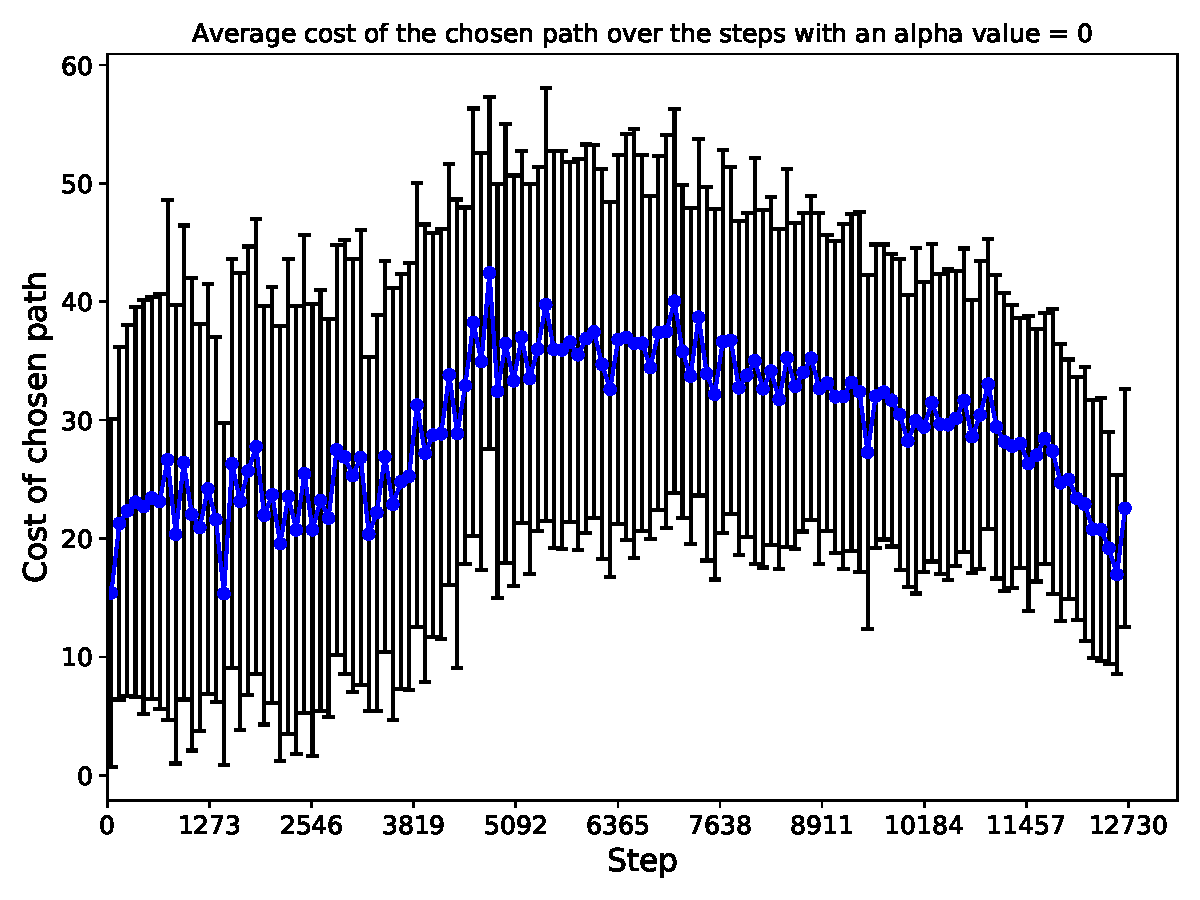
\includegraphics[width = .5\textwidth]{images/alpha_results/cost_alpha_0}} &
		\subfloat[Effetto di un valore del parametro $\alpha$ pari a 0.01 nella scelta della cella obiettivo in base al costo del cammino.\label{sfig:alphaCost0.01}]{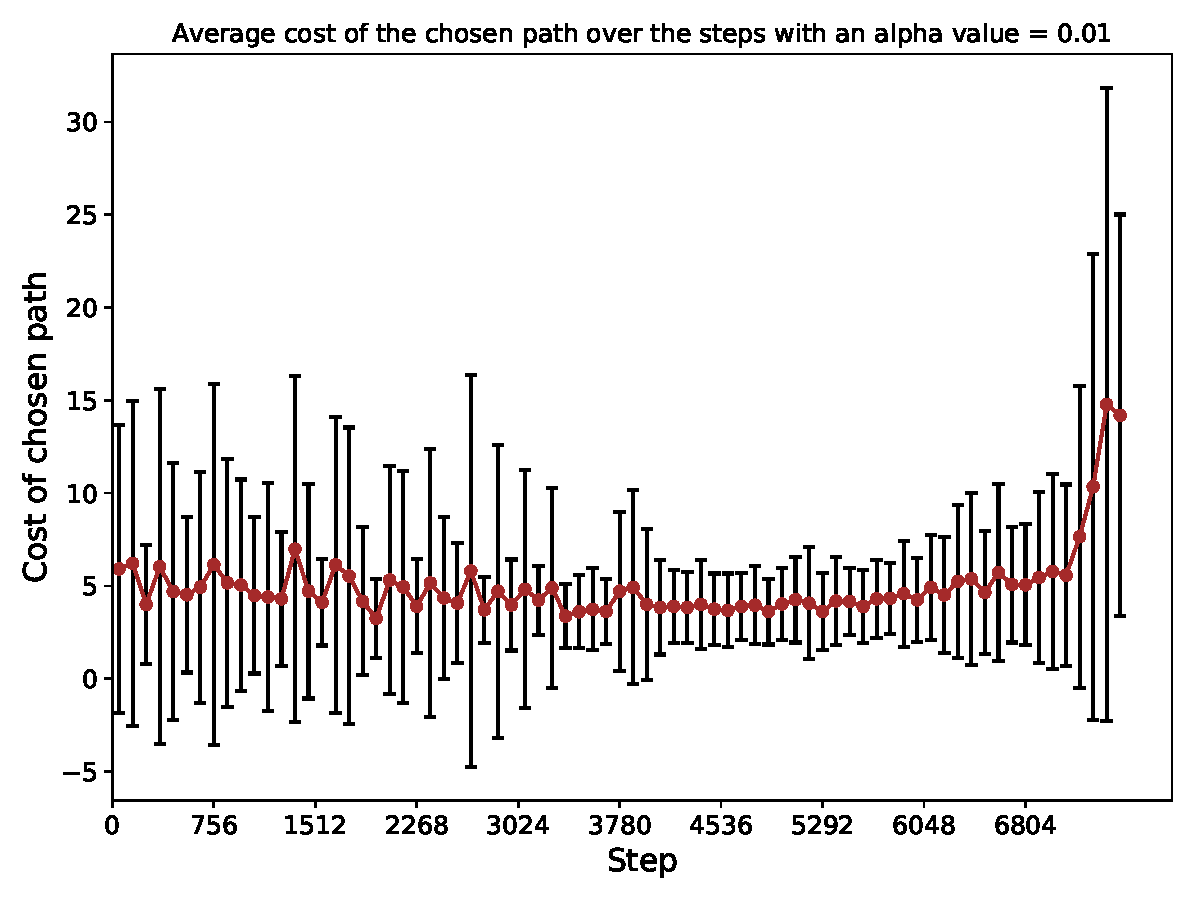
\includegraphics[width = .5\textwidth]{images/alpha_results/cost_alpha_0_01}}\\
		\subfloat[Effetto di un valore del parametro $\alpha$ pari a 6 nella scelta della cella obiettivo in base al costo del cammino.\label{sfig:alphaCost6}]{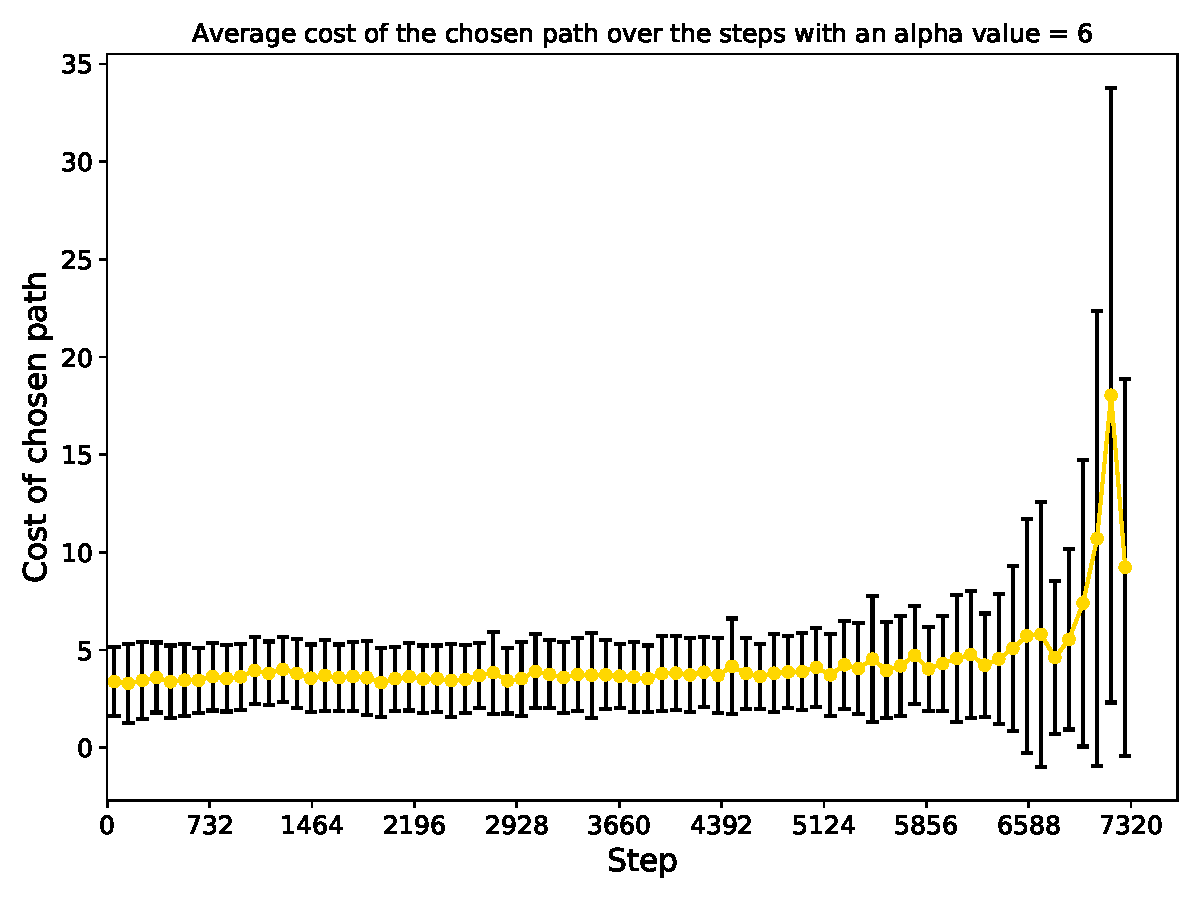
\includegraphics[width = .5\textwidth]{images/alpha_results/cost_alpha_6}} &
		\subfloat[Effetto di un valore del parametro $\alpha$ pari a 10 nella scelta della cella obiettivo in base al costo del cammino.\label{sfig:alphaCost10}]{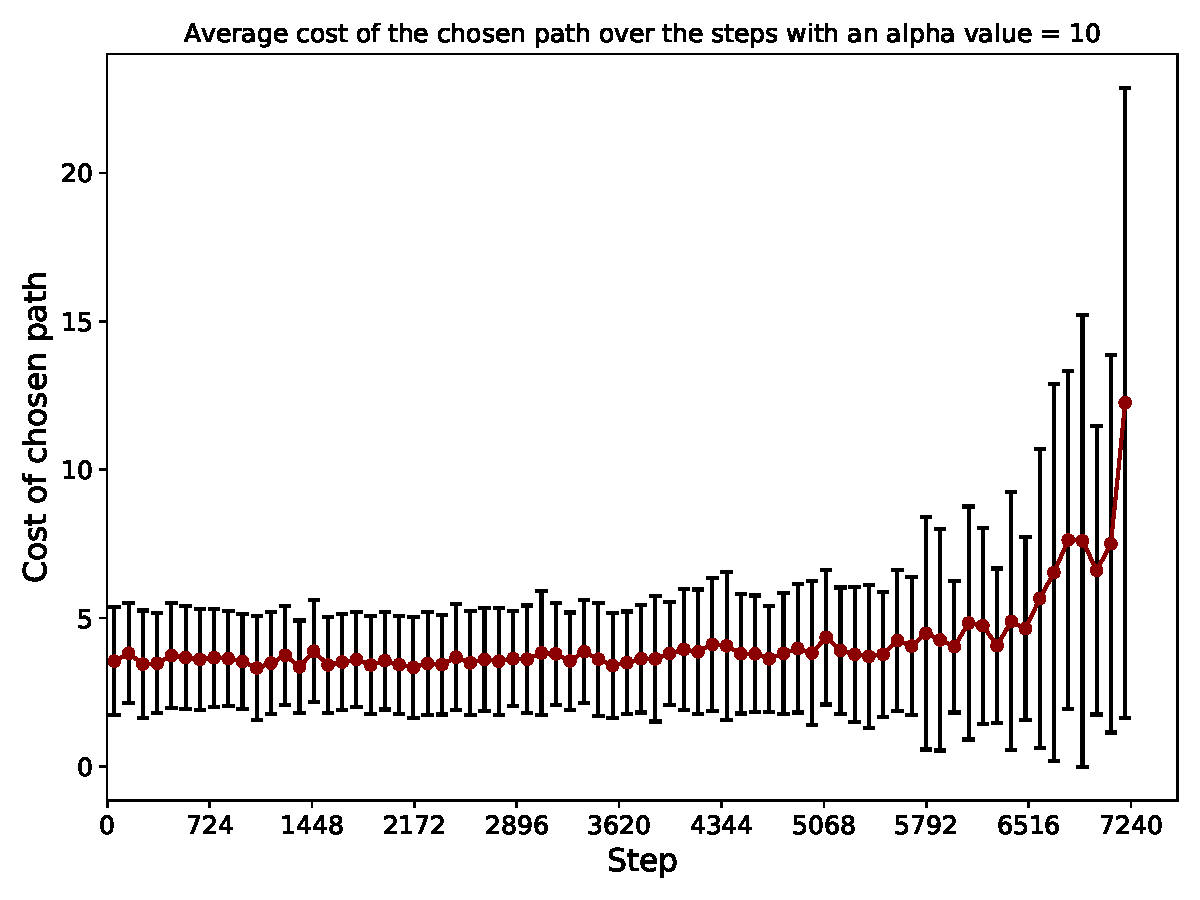
\includegraphics[width = .5\textwidth]{images/alpha_results/cost_alpha_10}}
	\end{tabular}
	\caption{In colore si denota la media dei costi dei cammini per raggiungere la cella scelta, i valori sono stati calcolati aggregando le scelte effettuate durante intervalli di 100 \textit{step}; in nero gli \textit{errorbar} relativi alla media determinati dalla deviazione standard.}
	\label{fig:alphaOverTime}
\end{figure}

\begin{figure}
	\centering
	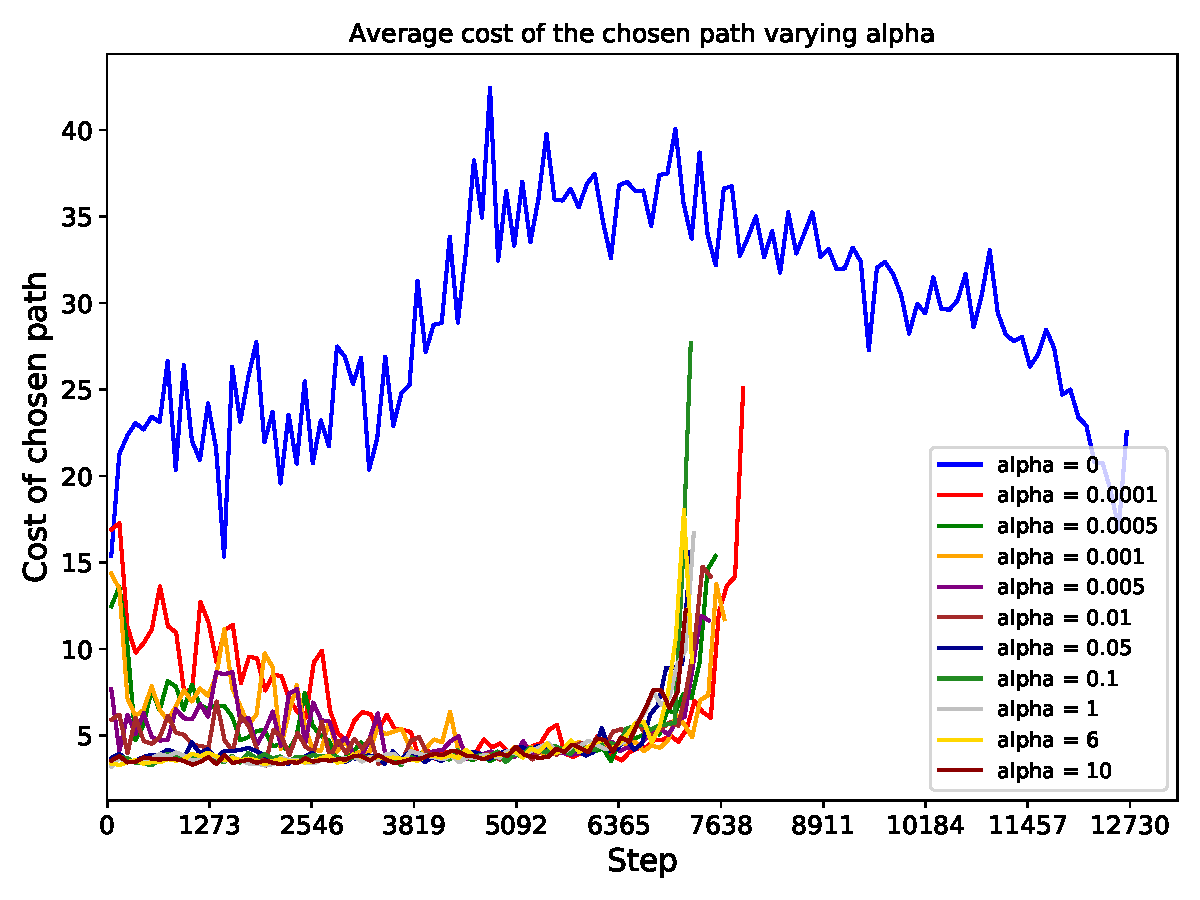
\includegraphics[width=0.9\linewidth]{images/alpha_results/comparison}
	\caption{Confronto tra la media dei costi dei cammini durante la simulazione per diversi valori di $\alpha$, anche in questo caso la media è stata calcolata in intervalli di 100 \textit{step}.}
	\label{fig:alphaComparison}
\end{figure}

\section{Analisi del parametro $\gamma$}
\label{sec:gamma}
Le analisi relative al parametro $\gamma$ sono state effettuate in maniera analoga a quelle precedenti: per ogni valore d'interesse di $\gamma$ sono state effettuate 10 simulazioni ognuna delle quali mantenendo invariati tutti gli altri parametri.
In particolare, le dimensioni della mappa sono state mantenute pari a 30$\times$30 celle, sono stati impiegati 6 robot con un raggio di visione pari a 6 celle, come suggerito dal processo di ottimizzazione descritto nel Capitolo \ref{chap:pso}, un raggio del ripetitore pari a 3 celle e abilitando i feriti a poter segnalare le loro posizioni.
Per quanto riguarda le mappe, sono state sfruttate le 5 mappe generate casualmente e utilizzate per le analisi condotte sul parametro $\alpha$ (Sezione \ref{sec:alpha}).
Infine, poiché ci si è accorti che il valore di $\alpha$ sia in grado di influenzare la distanza che mantengono tra loro i robot, si è deciso di effettuare due batterie di test: una prima in cui si è mantenuto un valore di $\alpha$ basso pari a $10^{-4}$ e poi per uno elevato pari a 8.175 (valore consigliato dal processo di ottimizzazione).
Le due batterie di test sono state eseguite in modo separato e autonomamente l'una dall'altra, non modificando altri parametri (escluso $\gamma$).\\
La metrica utilizzata per valutare come il parametro influisce nel comportamento del modello è stata la distanza media tra i robot. Come già detto, ci si aspetta che per valori alti di $\gamma$ gli agenti tendano a tenersi più distanti tra loro e viceversa.
Formalmente, la metrica viene computata nel seguente modo: per ogni robot si è calcolata la media delle distanze euclidee tra l'agente di interesse e tutti gli altri robot; in seguito, si è computata la media (e relativa deviazione standard) delle distanze medie.
Tale metrica è stata misurata ad ogni \textit{step} della simulazione.
Di seguito, mostriamo i principali risultati ottenuti in entrambe le batterie di test, ulteriori dati prodotti, meno significativi, sono riportati in Appendice \ref{apx:gamma}.

\subsection{Analisi con valore di $\alpha$ basso}
\label{subsec:gammaalow}
Una prima analisi effettuata è stata considerare per ogni valore del parametro la distribuzione della distanza media, ovvero in quanti \textit{step} si è presentato un determinato valore di distanza media; tali distribuzioni sono state calcolando aggregando i dati di tutte le simulazioni per ogni valore del parametro.
In Figura \ref{fig:gammaDistr} sono mostrate le distribuzioni per due valori di $\gamma$ (le altre sono riportate in Appendice \ref{apx:gamma}); si noti che la scala sull'asse delle \textit{y} è logaritmica e la distribuzione è rappresentata solo da un \textit{marker} che indica il numero di \textit{step} in cui si è verificate quel valore di distanza. Si tenga inoltre presente che i valori di distanza sono stati raggruppati per numeri interi.
Nelle distribuzioni mostrate, si nota come che per un valore di $\gamma$ pari a 0.32 (Figura \ref{sfig:gammaDistr0.32}), gli agenti tendano a mantenere una distanza nell'“intorno” di 30, con pochi casi di distanze pari o superiori a 50; al contempo, con un valore pari a 0.65 (Figura \ref{sfig:gammaDistr0.65}), si nota come non vi sia un valore di distanza che viene assunto significativamente più frequentemente di altri, ma il grafico presenta una distribuzione più “liscia”.\\
\begin{figure}
	\subfloat[Distribuzione della distanza media mantenuta dai robot con un valore di $\gamma$ pari a 0.32.\label{sfig:gammaDistr0.32}]{
		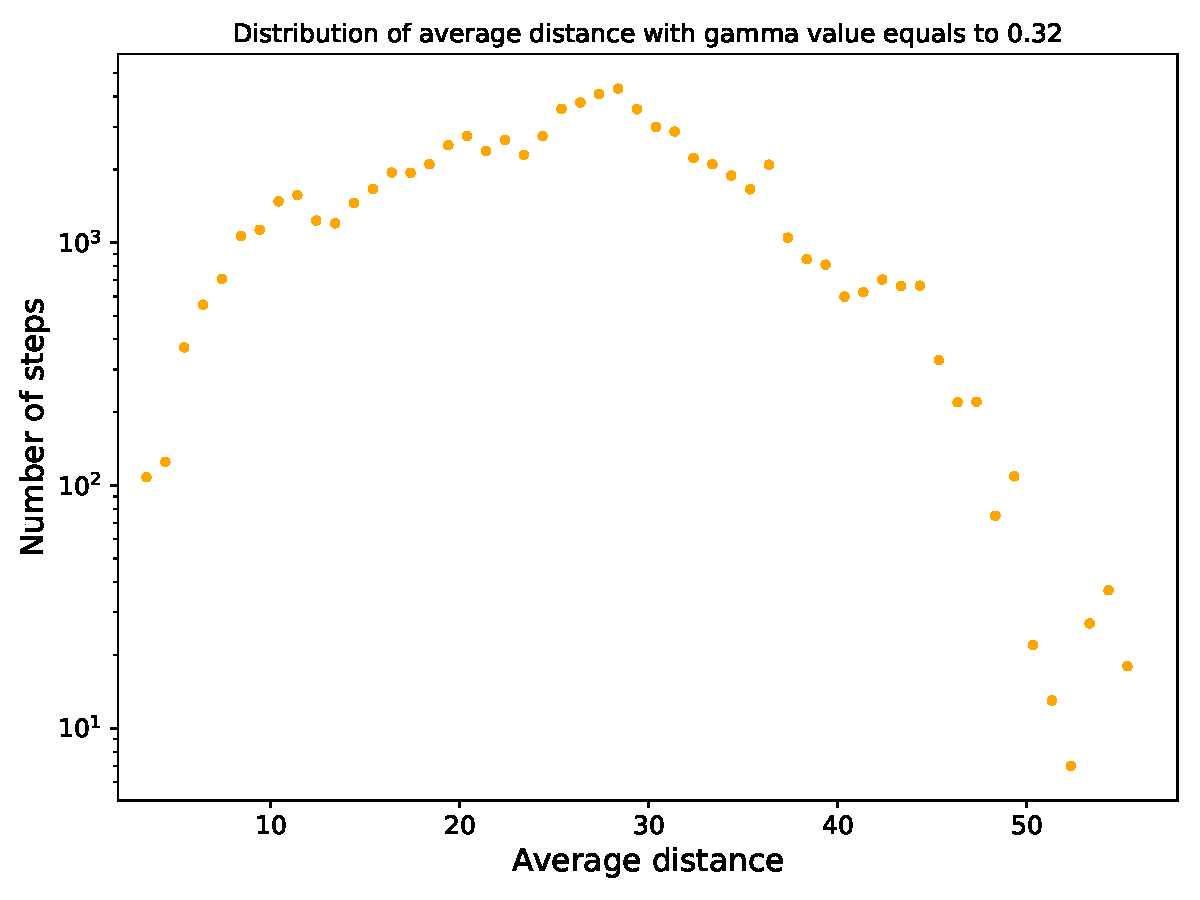
\includegraphics[width=.47\linewidth]{images/gamma_results/low_alpha/distribution_distance_gamma_0_32}
	}
	\hfill
	\subfloat[Distribuzione della distanza media mantenuta dai robot con un valore di $\gamma$ pari a 0.65.\label{sfig:gammaDistr0.65}]{
		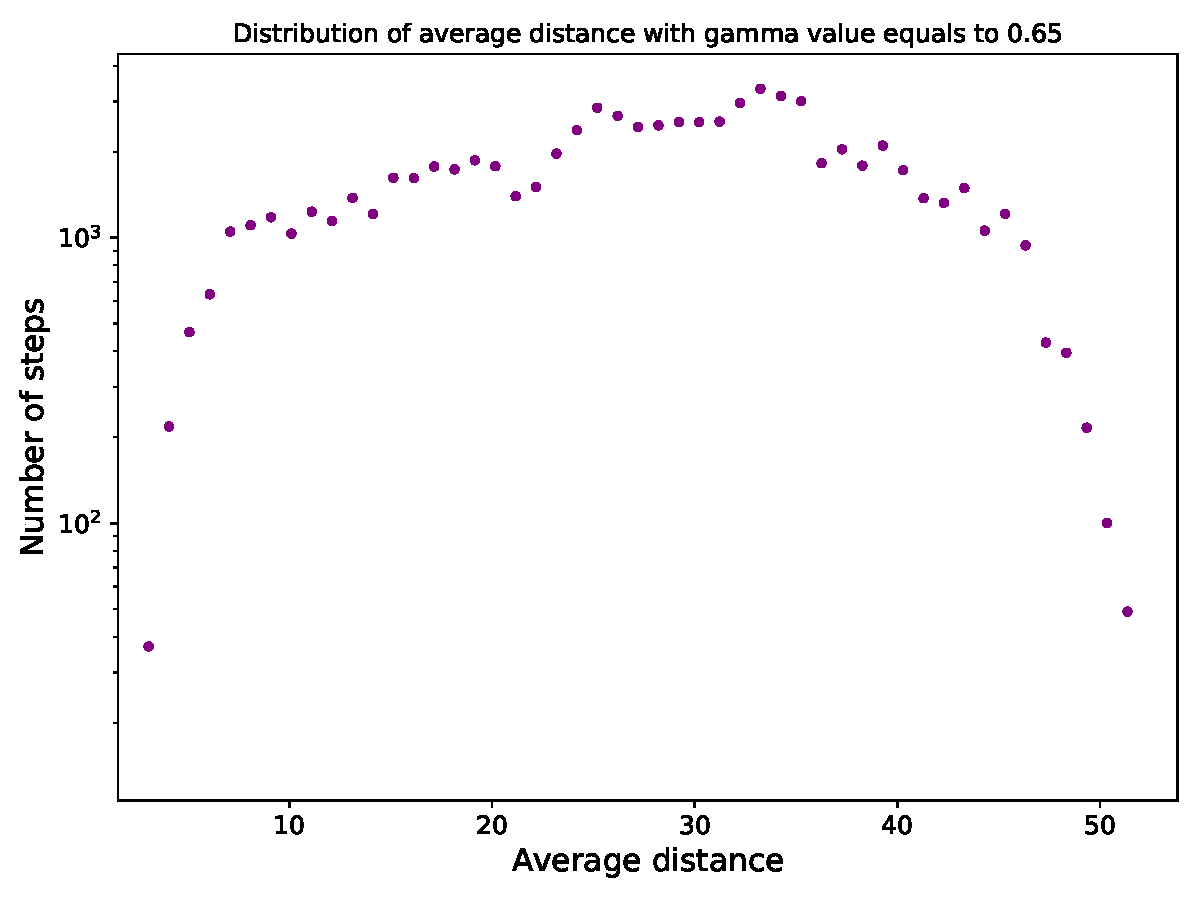
\includegraphics[width=.47\linewidth]{images/gamma_results/low_alpha/distribution_distance_gamma_0_65}
	}
	\caption{Distribuzione della distanza media mantenuta dai robot al variare del valore di $\gamma$, per valutare la distribuzione si è conteggiato in quanti \textit{step} i robot hanno presentato tale distanza, il numero di \textit{bin} per produrre la distribuzione è pari alla differenza tra la distanza minima e massima presente durante la simulazione, tale valore è stato poi arrotondato. Infine si noti che l'asse delle \textit{y} è a scala logaritmica.}
	\label{fig:gammaDistr}
\end{figure}
Poiché effettuare dei confronti solo mediante grafici di distribuzioni realizzati ognuno per ogni valore analizzato di $\gamma$ risulta complicato e poco significativo, si è deciso di confrontarli unendo tali distribuzioni nello stesso grafico; si noti che l'asse delle \textit{y} non è più a scala logaritmica, in modo da favorire un confronto qualitativo delle distribuzioni.
Il grafico complessivo, riportato in Figura \ref{fig:gammaComparison}, mostra come al crescere de valore $\gamma$ la distanza media tra gli agenti tende ad aumentare per un numero maggiore di \textit{step}.
In particolare si può notare come che per valori di $\gamma$ pari a 0.32 e 1 si presentino dei veri e propri “picchi”; è interessante che per il valore pari a 0.65 non vi sia un vero e proprio “picco” ma, come già detto, la distribuzione risulti più “liscia”, presentando al contempo un numero maggiore di \textit{step} con distanze medie tra 40 e 50 (che risultano essere distanze elevate) e che non compaiono in modo così significativo per nessun altro valore di $\gamma$.
Per valori bassi di $\gamma$ non si evidenziano significative differenze in termini di distanza, ma comunque tende ad emergere una concentrazione di valori di distanza relativamente bassi rispetto agli altri valori di $\gamma$.
In particolare, valutando con attenzione la Formula \ref{math:utility-red} grazie a cui l'utilità di una cella viene ridotta, possiamo intuire che un valore basso di $\gamma$ porta tutte le celle percepite dal robot ad avere un'utilità molto simile e prossima allo $0$. Viceversa, un valore alto di $\gamma$ genera una netta differenza tra celle immediatamente circostanti alla posizione e celle più lontane, garantendo un'efficace meccanismo di dissuasione per gli altri robot.\\
Riassumendo quanto valutato fin'ora, si nota come con un valore di $\alpha$ basso, il parametro $\gamma$ influenza la distanza tra gli agenti, presentando un comportamento particolare per il valore di $\gamma$ pari a 0.65 che è stato quello suggerito dal processo di ottimizzazione (si faccia riferimento al Capitolo \ref{chap:pso}).
\begin{figure}
	\centering
	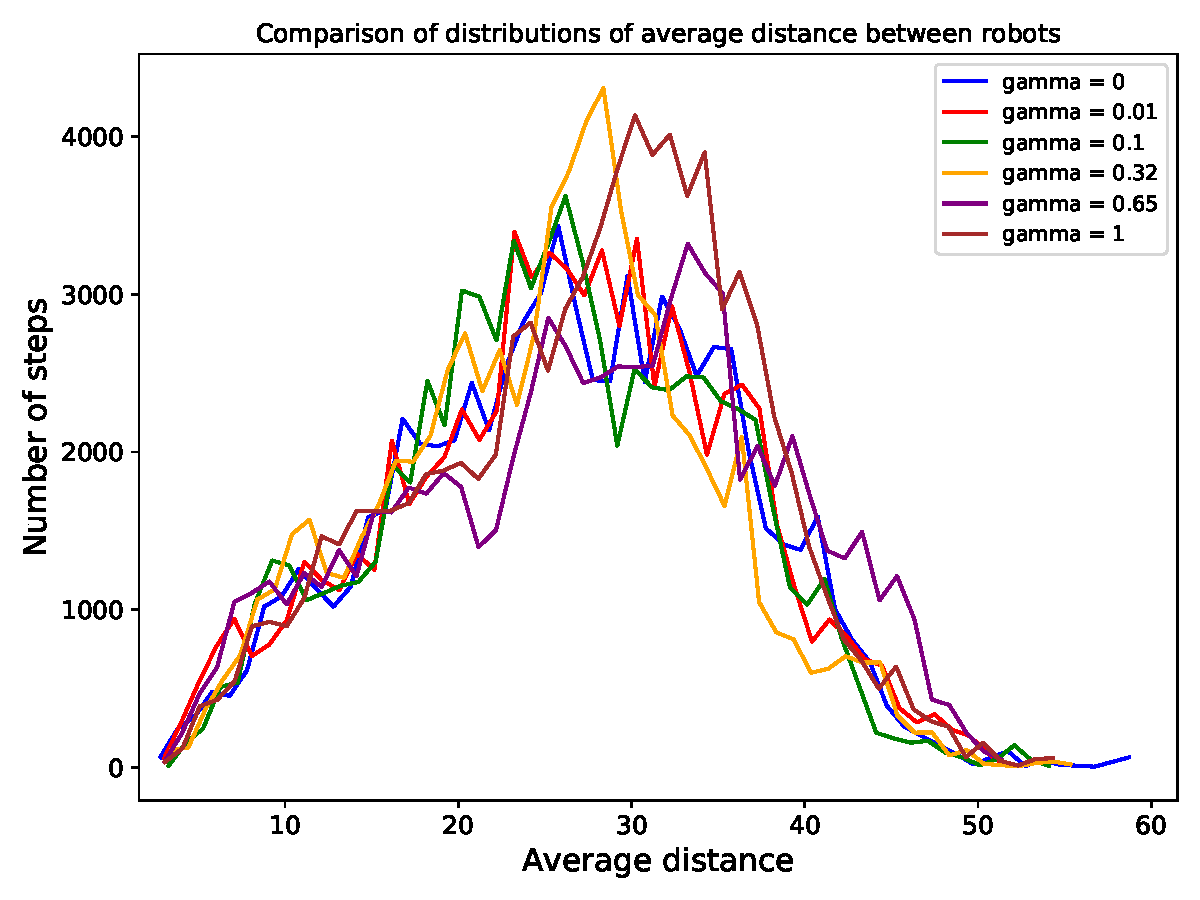
\includegraphics[width=0.9\linewidth]{images/gamma_results/low_alpha/comparison}
	\caption{Grafico che riassume tutte le distribuzioni di distanze medie durante le simulazioni per ogni valore di $\gamma$, si noti che l'asse delle \textit{y} non è più logaritmico.}
	\label{fig:gammaComparison}
\end{figure}

Infine, \margin{Come $\alpha$ influenza la distanza tra gli agenti}si è andati a studiare l'evolversi all'interno della singola simulazione (ne è stata scelta una casualmente tra le dieci eseguite per ogni valore di $\gamma$ studiato) della distanza media tra i robot.
Tali evoluzioni sono mostrate in Figura \ref{fig:gammaSim} per quanto riguarda i valori del parametro pari a 0.32 (Figura \ref{sfig:gammaSim0.32}) e 0.65 (Figura \ref{sfig:gammaSim0.65}), per gli altri si faccia riferimento all'Appendice \ref{apx:gamma}.
In entrambe le simulazioni emerge come più di una volta la distanza tra gli agenti sia diminuita drasticamente e repentinamente per poi, dopo pochi \textit{step}, ricominciare ad aumentare.
Si è associato tale fenomeno alla possibilità da parte dei feriti di segnalarsi, in particolare, ogni volta che qualcuno si segnala, la priorità delle celle del vicinato viene incrementata, e quindi incrementa l'\textit{info-gain} di tali celle.
Notiamo però che questo fenomeno sembra essere meno presente mano a mano che gamma cresce: questo è probabilmente dovuto al fatto che, al crescere di gamma, l'utilità delle celle nell'intorno di una cella che viene esplorata è fortemente diminuito, mentre le celle più distanti subiscono meno questo malus. Nella scelta della cella bersaglio, essendo $\alpha$ molto basso, la differenza tra utilità e priorità di una cella potrebbe propendere verso la prima componente, rendendo quindi una cella proritizzata vicina a una cella già esplorata meno interessante di una priva di priorità ma più distante.
Poiché il valore di $\alpha$ è basso, i robot non faranno pesare in maniera significativa il costo del cammino e quindi, anche se distanti, tenderanno a scegliere tali celle, portando quindi ad un avvicinamento dei robot con lo scopo di esplorare completamente (e in poco tempo) tutta l'area attorno a dove si è segnalato un ferito.
\begin{figure}
	\subfloat[Evoluzione della distanza media tra gli agenti con un valore di $\gamma$ pari a 0.32.\label{sfig:gammaSim0.32}]{
		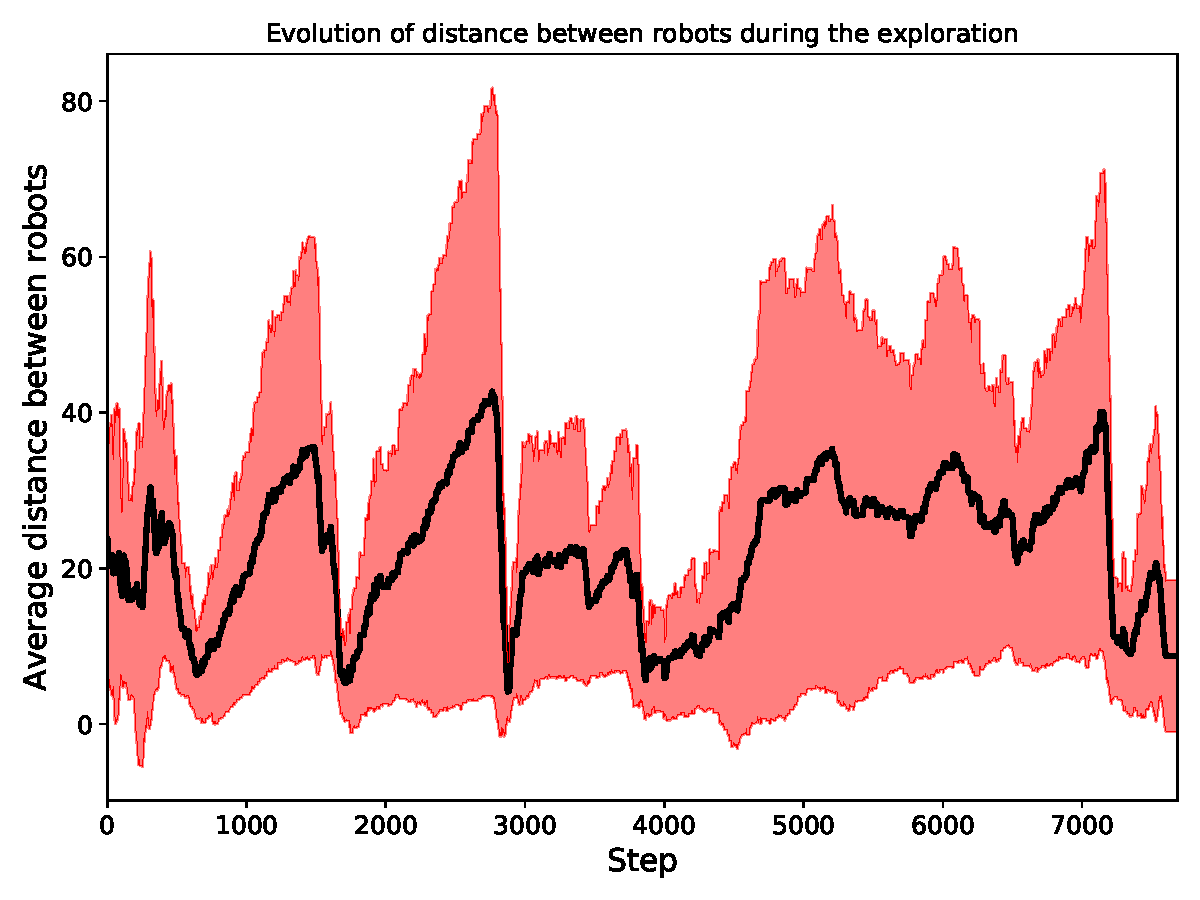
\includegraphics[width=.47\linewidth]{images/gamma_results/low_alpha/dinstance_simulation_gamma_0_32_simid_0}
	}
	\hfill
	\subfloat[Evoluzione della distanza media tra gli agenti con un valore di $\gamma$ pari a 0.65.\label{sfig:gammaSim0.65}]{
		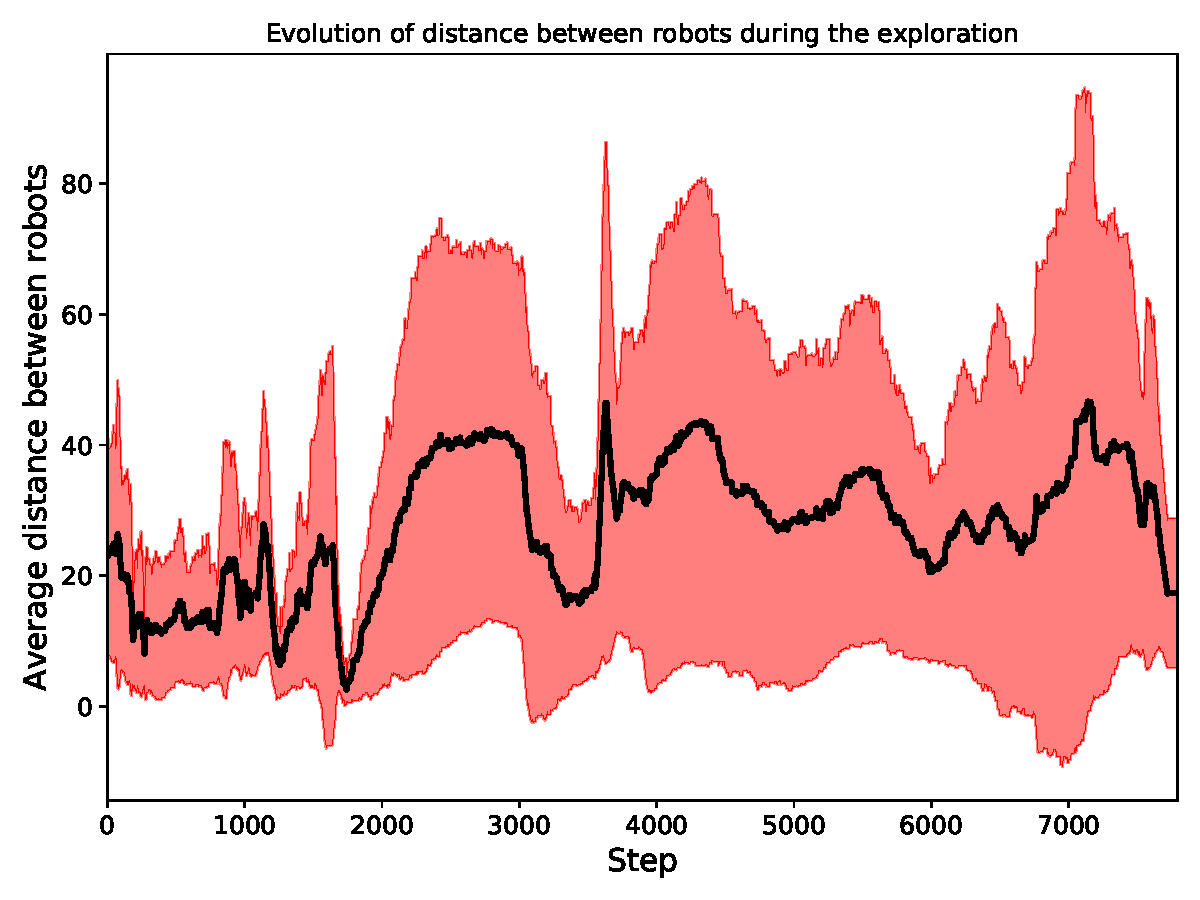
\includegraphics[width=.47\linewidth]{images/gamma_results/low_alpha/dinstance_simulation_gamma_0_65_simid_0}
	}
	\caption{Sull'asse delle \textit{x} si trova il tempo, in termini di \textit{step}, impiegato per l'esplorazione della mappa, mentre sull'asse delle \textit{y} la distanza media tra gli agenti.}
	\label{fig:gammaSim}
\end{figure}

\subsection{Analisi con valore di $\alpha$ alto}
\label{subsec:gammaahigh}
Come in precedenza, le prime analisi effettuate si sono concentrate sulla distribuzione delle distanze medie.
In Figura \ref{fig:gammaHDistr} sono rappresentate le due distribuzioni per i valori di $\gamma$ considerati in precedenza; si può notare che con valori alti di $\alpha$, l'andamento della distribuzione si sia invertita rispetto al caso precedente: per un valore pari a 0.32 (Figura \ref{sfig:gammaHDistr0.32}) la distribuzione sembra essere più “liscia”, invece per un valore pari a 0.65 (Figura \ref{sfig:gammaHDistr0.65}) o superiore sembra infittirsi per alcuni valori di distanza.
\begin{figure}
	\subfloat[Distribuzione della distanza media mantenuta dai robot con un valore di $\gamma$ pari a 0.32.\label{sfig:gammaHDistr0.32}]{
		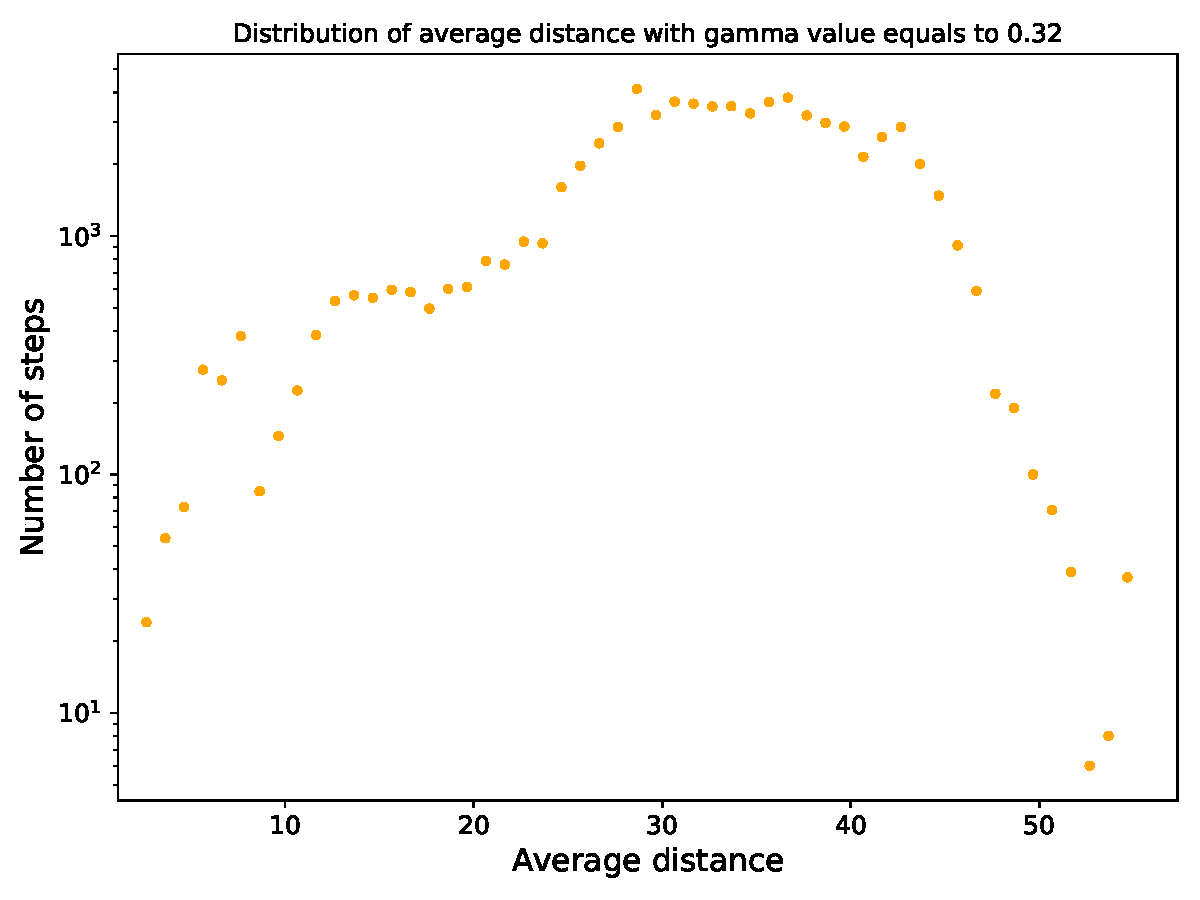
\includegraphics[width=.47\linewidth]{images/gamma_results/high_alpha/distribution_distance_gamma_0_32}
	}
	\hfill
	\subfloat[Distribuzione della distanza media mantenuta dai robot con un valore di $\gamma$ pari a 0.65.\label{sfig:gammaHDistr0.65}]{
		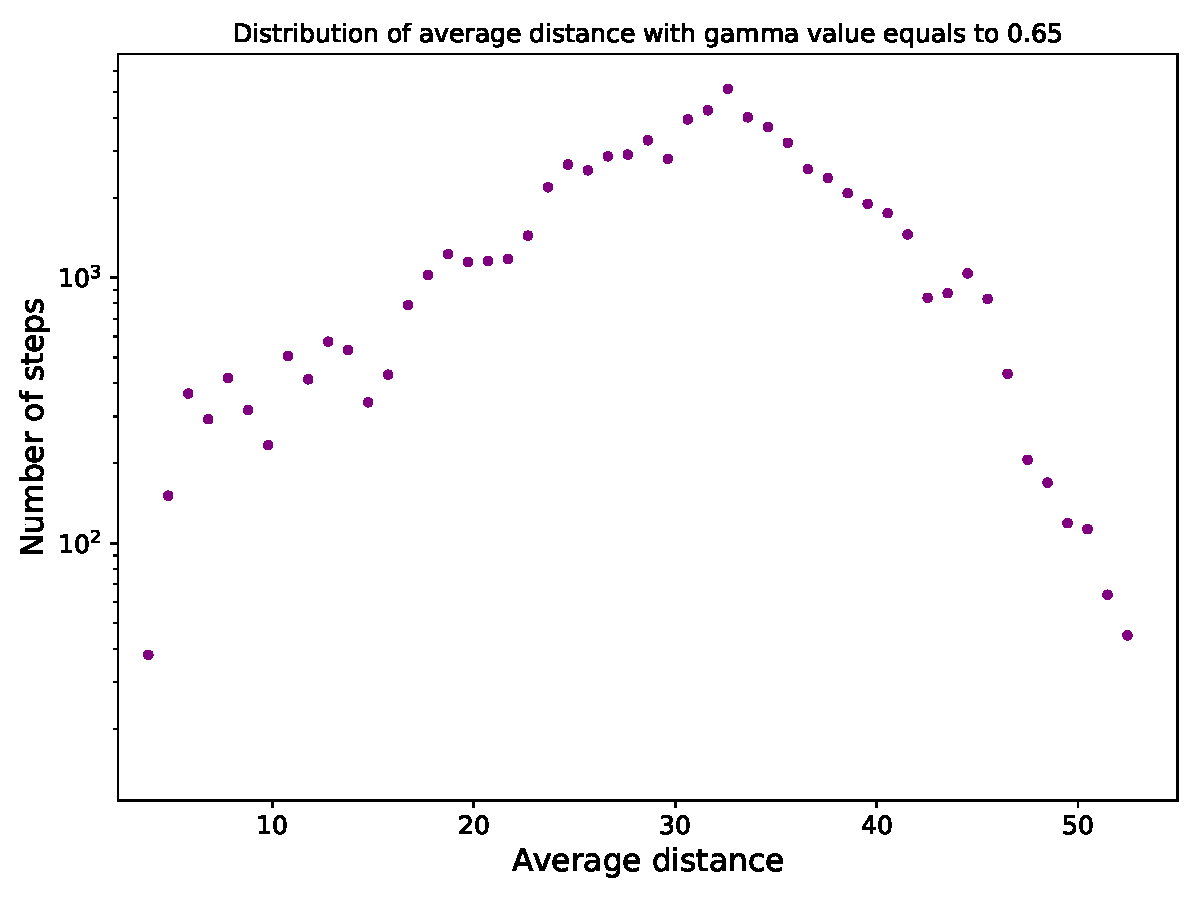
\includegraphics[width=.47\linewidth]{images/gamma_results/high_alpha/distribution_distance_gamma_0_65}
	}
	\caption{Distribuzione della distanza media mantenuta dai robot al variare del valore di $\gamma$, per valutare la distribuzione si è conteggiato in quanti \textit{step} i robot hanno presentato tale distanza, il numero di \textit{bin} per produrre la distribuzione è pari alla differenza tra la distanza minima e massima presente durante la simulazione, tale valore è stato poi arrotondato. Infine si noti che l'asse delle \textit{y} è a scala logaritmica.}
	\label{fig:gammaHDistr}
\end{figure}
Ancora una volta si è deciso di andare a confrontare tutte le distribuzioni dei valori del parametro analizzati, i risultati sono mostrati in Figura \ref{fig:gammaHComparison}.
Come si può notare, al contrario del caso precedente, per valori pari a 0.65 o 1 si notano dei “picchi” significativi e anche per valori più bassi (0.1 e 0.32) si nota come i robot mantengano una distanza media maggiore; tale risultato sembra contraddire quello detto in precedenza.\\
Per analizzare meglio questi risultati e introdurli nel quadro complessivo, bisogna considerare che non è solo $\gamma$ (come avveniva di fatto precedentemente) ad influire sulla scelta della cella obiettivo e degli spostamenti del robot, ma risulta essere vincolante anche il costo del cammino. 
Poiché il parametro $\alpha$ influisce significativamente e con una magnitudo molto maggiore rispetto all'utilità e priorità della cella nella scelta del bersaglio, il parametro $\gamma$ passa in secondo piano e influisce solo in maniera marginale sulla scelta. Ciò va ad inficiare la distanza tra i robot, poiché tali scelte non vengono più effettuate dando grande importanza all'utilità della cella quanto al tempo necessario per raggiungerla.
\begin{figure}
	\centering
	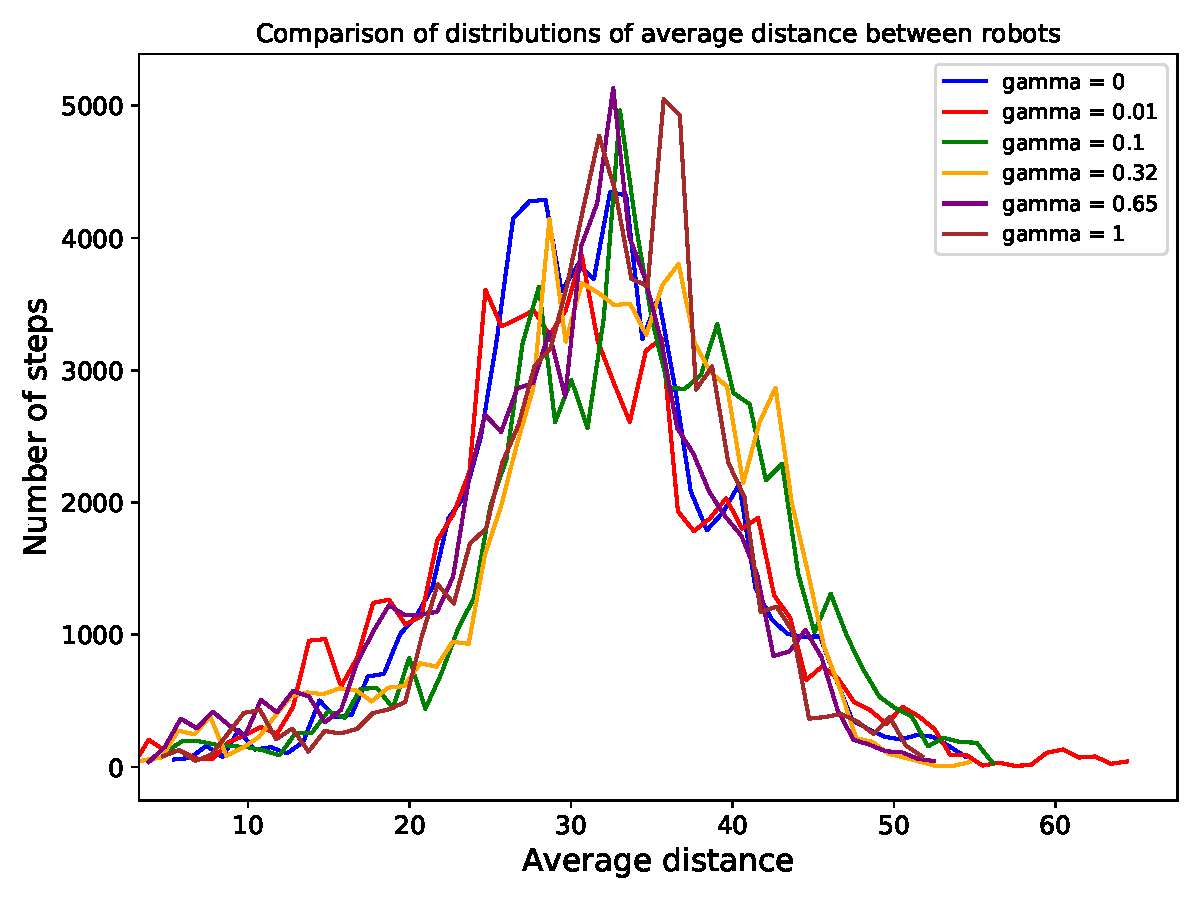
\includegraphics[width=0.9\linewidth]{images/gamma_results/high_alpha/comparison}
	\caption{Grafico che riassume tutte le distribuzioni di distanze medie durante le simulazioni per ogni valore di $\gamma$, si noti che l'asse delle \textit{y} non è più logaritmico.}
	\label{fig:gammaHComparison}
\end{figure}
Come ulteriore conferma di tale affermazione, si può notare come durante la singola simulazione non si presentino più quelle situazioni in cui la distanza tra i robot decresce significativamente a causa della segnalazione da parte dei feriti. Solo durante le fasi finali dell'esplorazione la distanza tra essi alle volte diminuisce.
Al fine di evitare che i feriti vengano di fatto ignorati, è stata implementata una seconda tecnica di prioritizzazione delle celle che, al posto di utilizzare un valore fisso stabilito a priori, utilizza un valore dipendente da $\alpha$; i risultati di tale metodo, discusso nella Sotto-sezione \ref{Ferito} saranno discussi tra breve.
L'evolversi delle distanze è rappresentato in Figura \ref{fig:gammaHSim}
\begin{figure}
	\subfloat[Evoluzione della distanza media tra gli agenti con un valore di $\gamma$ pari a 0.32.]{
		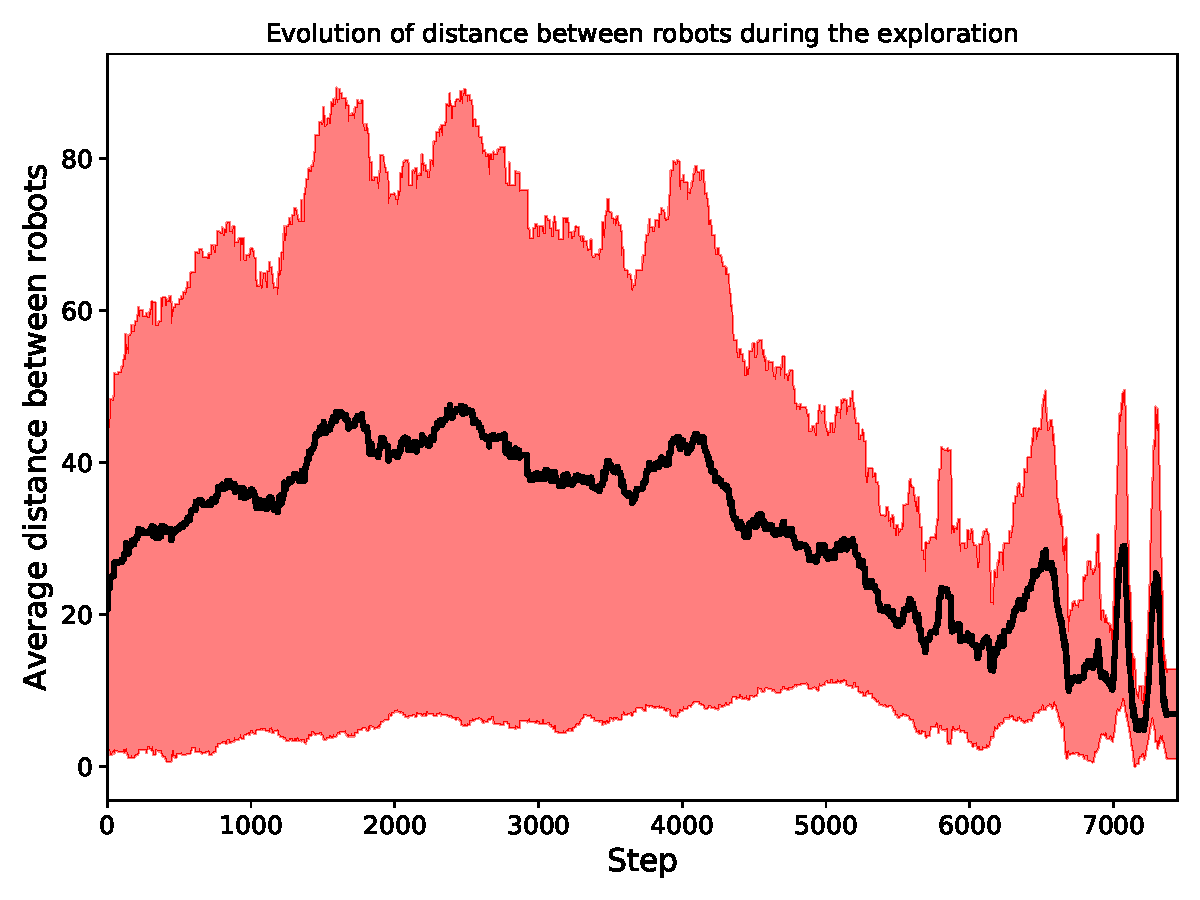
\includegraphics[width=.47\linewidth]{images/gamma_results/high_alpha/dinstance_simulation_gamma_0_32_simid_0}
	}
	\hfill
	\subfloat[Evoluzione della distanza media tra gli agenti con un valore di $\gamma$ pari a 0.65.]{
		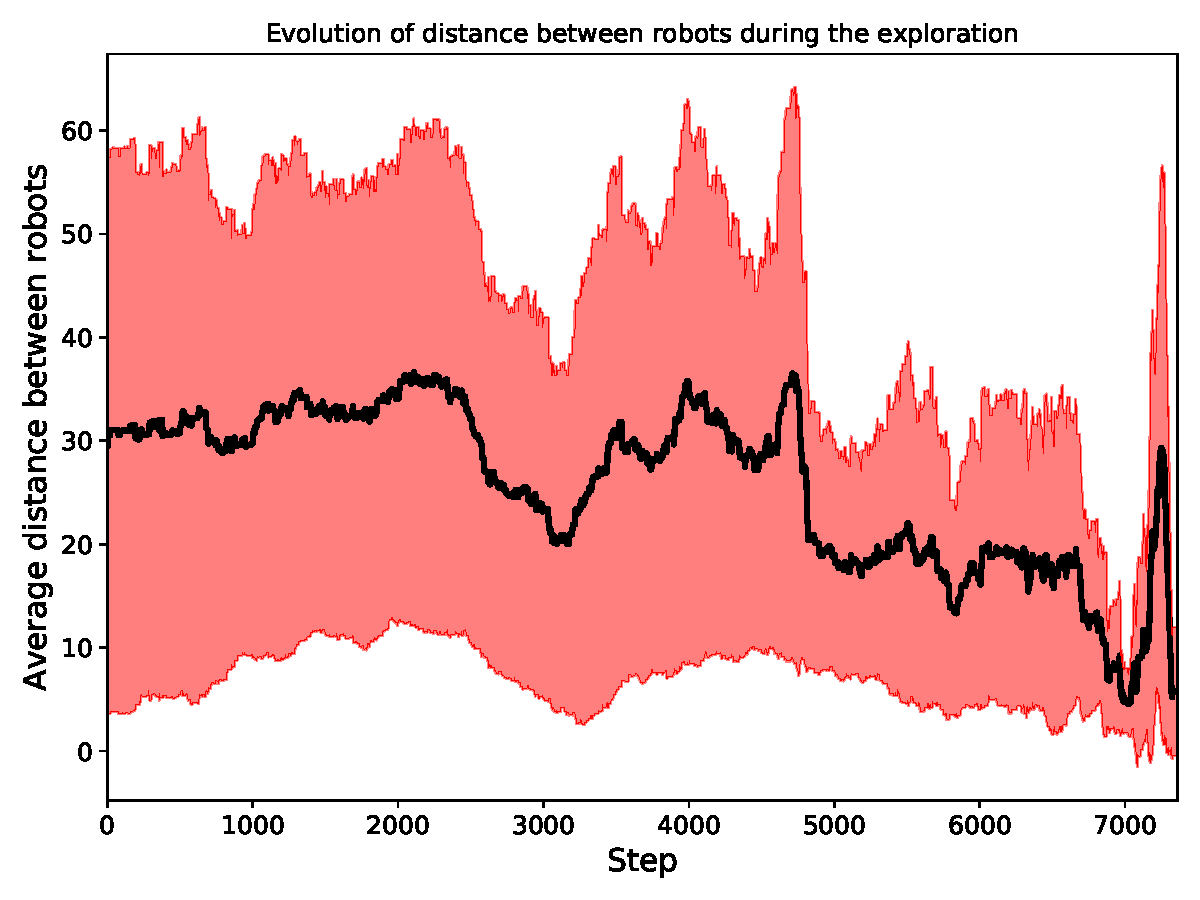
\includegraphics[width=.47\linewidth]{images/gamma_results/high_alpha/dinstance_simulation_gamma_0_65_simid_4}
	}
	\caption{Sull'asse delle \textit{x} si trova il tempo, in termini di \textit{step}, impiegato per l'esplorazione della mappa, mentre sull'asse delle \textit{y} la distanza media tra gli agenti.}
	\label{fig:gammaHSim}
\end{figure}
\subsection{Considerazioni conclusive}
In questo breve sunto, si vogliono evidenziare alcune differenze tra come opera il parametro $\gamma$ rispetto al valore di $\alpha$.
In particolare, si è notato come per valori di $\alpha$ bassi è effettivamente il parametro $\gamma$ ad influire sulla distanza tra i robot portando questi a scegliere le celle con utilità maggiore (poiché il peso influisce in maniera poco significativa) e quindi scegliendo le celle viste da meno robot (poiché sono quelle che hanno subito meno riduzioni di utilità).
In aggiunta, si evidenzia come per valori di $\alpha$ bassi i robot tenderanno a muoversi tutti verso la zona segnalata da un ferito nel momento in cui questi segnalano la loro presenza; al contempo, tale effetto sembra più marginale nel momento in cui $\alpha$ aumenta.
Nonostante queste considerazioni, si nota comunque come per valori di $\gamma$ elevati gli agenti, in entrambi i casi, tendono a rimanere più distanti rispetto a valori bassi (si tenga presente che i “picchi” per $\alpha$ elevati sono presenti per valori di distanza minori).
Ancora una volta, tale fenomeno è dovuto al fatto che quando il costo del cammino è maggiormente significativo nel calcolo dell'\textit{info-gain} diventa il principale parametro che delinea la scelta e quindi riducendo l'effetto dell'utilità delle celle e di conseguenza l'influenza del parametro $\gamma$.
\subsection{Metodo di prioritizzazione alternativo}
Al fine di indagare come il metodo di prioritizzazione alternativo, proposto nella Sotto-sezione \ref{subsec:Ferito}, fosse in grado di modificare il comportamento dei robot negli scenari analizzati in precedenza, sono stati ripetuti i medesimi test utilizzando però la forma di priorità che tiene conto del valore di $\alpha$. Questo dovrebbe portare i robot a evitare situazioni in cui l'intera flotta si raduna in un unico punto a seguito della segnalazione della presenza di un ferito (comportamento evidenziato con valori di $\alpha$ bassi).
Come mostrato nella Figura \ref{fig:NgammaLDistr}, i dati sembrano confermare quanto supposto. Non sono più evidenti decrescite repentine che portano i robot a raggrupparsi in una medesima area, come era invece mostrato nell'analisi corrispettiva eseguita con il precedente metodo di prioritizzazione (Figura \ref{fig:gammaSim})
\begin{figure}
	\subfloat[Evoluzione della distanza media tra gli agenti con un valore di $\gamma$ pari a 0.32.]{
		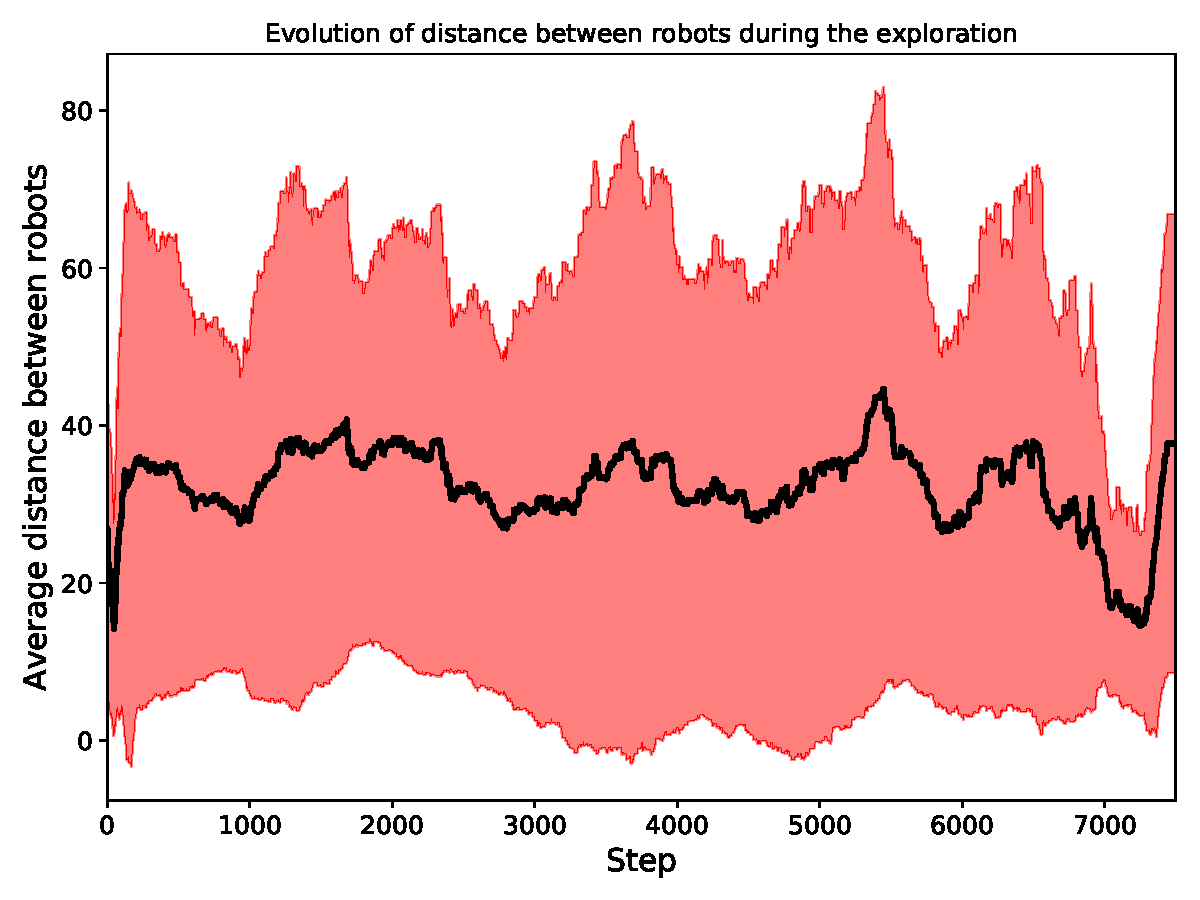
\includegraphics[width=.47\linewidth]{images/high_priority_gamma_results/low_alpha/dinstance_simulation_gamma_0_32}
	}
	\hfill
	\subfloat[Evoluzione della distanza media tra gli agenti con un valore di $\gamma$ pari a 0.65.]{
		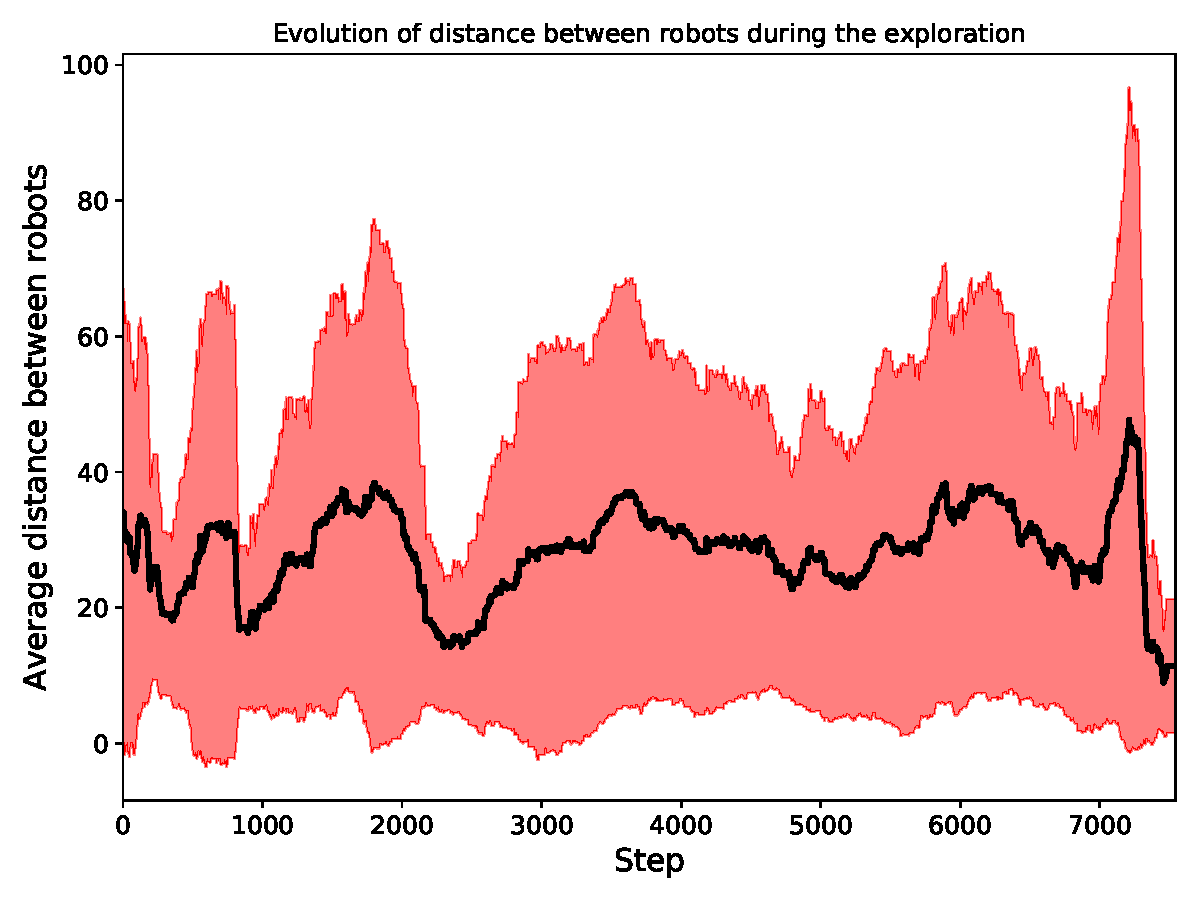
\includegraphics[width=.47\linewidth]{images/high_priority_gamma_results/low_alpha/dinstance_simulation_gamma_0_65}
	}
	\caption{Sull'asse delle \textit{x} si trova il tempo, in termini di \textit{step}, impiegato per l'esplorazione della mappa, mentre sull'asse delle \textit{y} la distanza media tra gli agenti.}
	\label{fig:NgammaLDistr}
\end{figure}
Al contempo, analizzando il grafico comparativo delle distribuzioni di distanza tra i robot ad ogni \textit{step}, riportato in Figura \ref{fig:NgammaLComparison}, vediamo come vi sia un'effettiva minore distanza media per valori di $\gamma$ prossimi a zero rispetto agli altri casi. Questo avvalora la tesi già enunciata in precedenza che sostiene che valori di gamma prossimi al valore nullo portano tutte le celle nel vicinato della cella obiettivo, anche quelle molto distanti, ad avere utilità simile e prossima a zero. Ciò porta il costo del cammino minimo verso l'obiettivo a diventare nuovamente protagonista nel calcolo dell'\textit{info-gain}, rendendo vana la tecnica di repulsione tra robot così implementata.
\begin{figure}
	\centering
	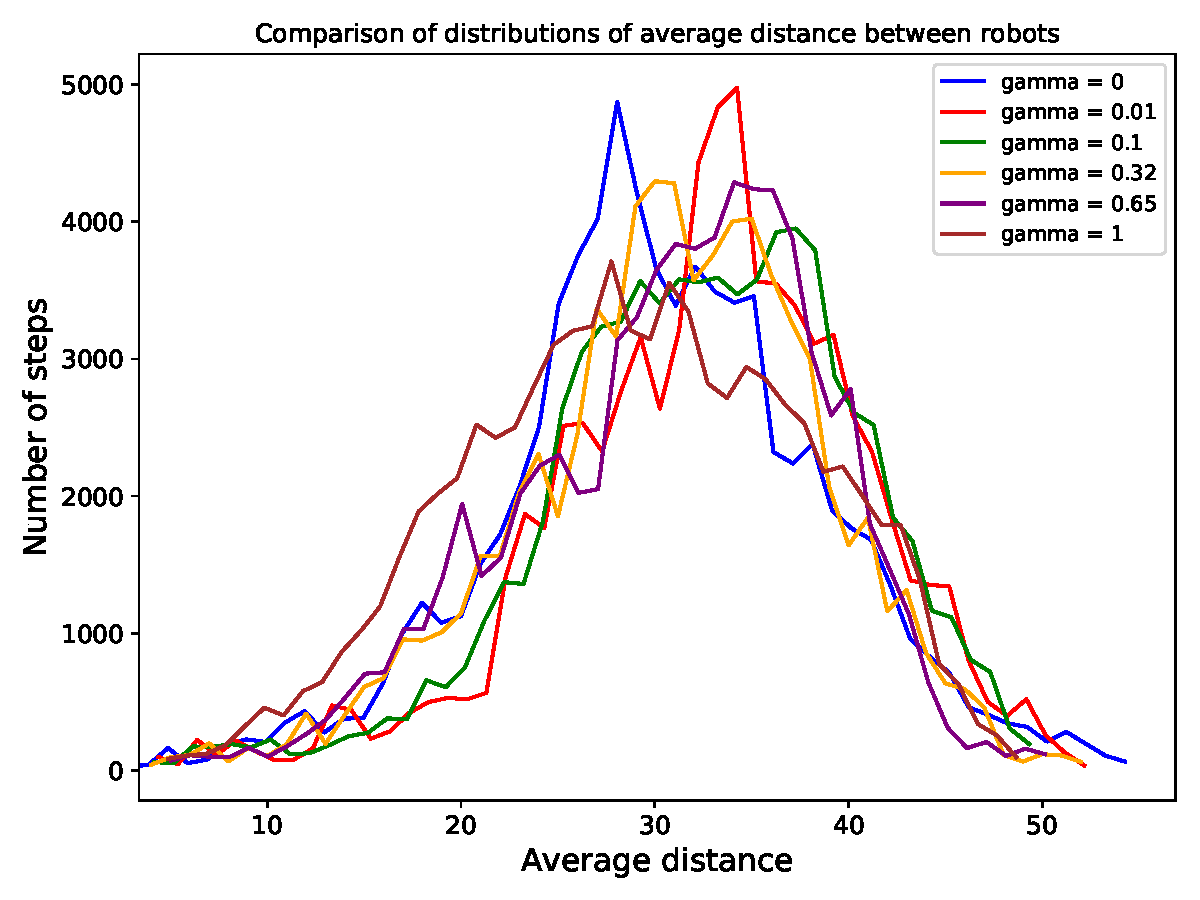
\includegraphics[width=0.9\linewidth]{images/high_priority_gamma_results/low_alpha/comparison}
	\caption{Grafico che riassume tutte le distribuzioni di distanze medie durante le simulazioni per ogni valore di $\gamma$, si noti che l'asse delle \textit{y} non è più logaritmico.}
	\label{fig:NgammaLComparison}
\end{figure}
Per quanto concerne i dati ottenuti con valori di $\alpha$ più elevati, i risultati e le conclusioni sono assimilabili a quelle appena tratte per valori del parametro inferiori (tutti i grafici sono disponibili nell'Appendice \ref{apx:gamma}).

\section{Stato dei robot}
\chapter{Conclusioni}


\begin{appendices}
	\chapter{Ulteriori risultati su come il parametro $\alpha$ influisce nel costo del cammino}
	\label{apx:alpha}
	In questo appendice, si mostrano brevemente i grafici che non sono stati inseriti direttamente nel Sezione \ref{sec:alpha}, dove sono stati discussi gli effetti che ha il parametro $\alpha$ nella scelta dei costi dei cammini.
In particolare, nelle Figure \ref{figapx:alpha1} e \ref{figapx:alpha2} sono riportati i grafici contenenti i costi dei cammini scelti durante la simulazione (aggregati ogni 100 \textit{step} della simulazione).

\begin{figure}
	\begin{tabular}{cc}
		\subfloat[Effetto di un valore del parametro $\alpha$ pari a $10^{-4}$ nella scelta della cella obiettivo in base al costo del cammino.]{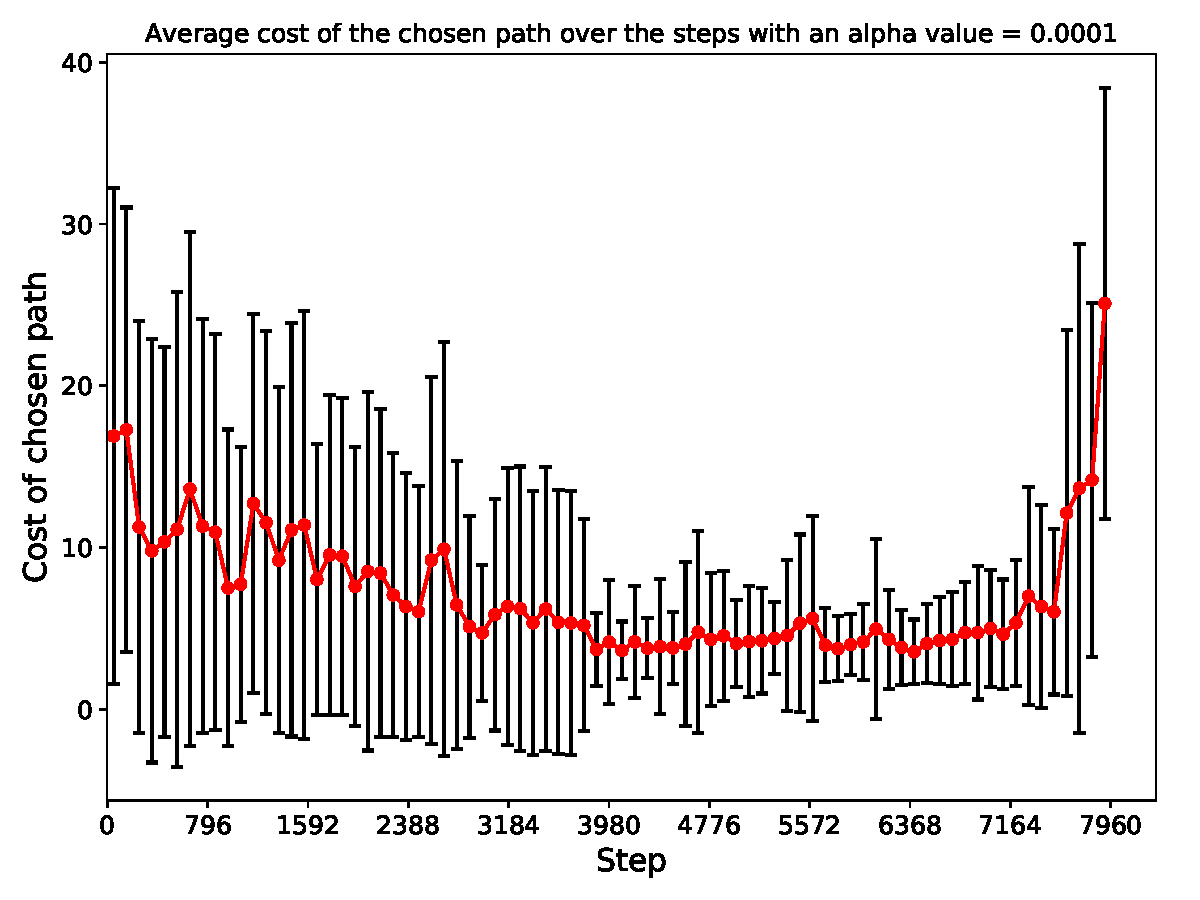
\includegraphics[width = .5\textwidth]{images/alpha_results/cost_alpha_0_0001}} &
		\subfloat[Effetto di un valore del parametro $\alpha$ pari a 0.0005 nella scelta della cella obiettivo in base al costo del cammino.]{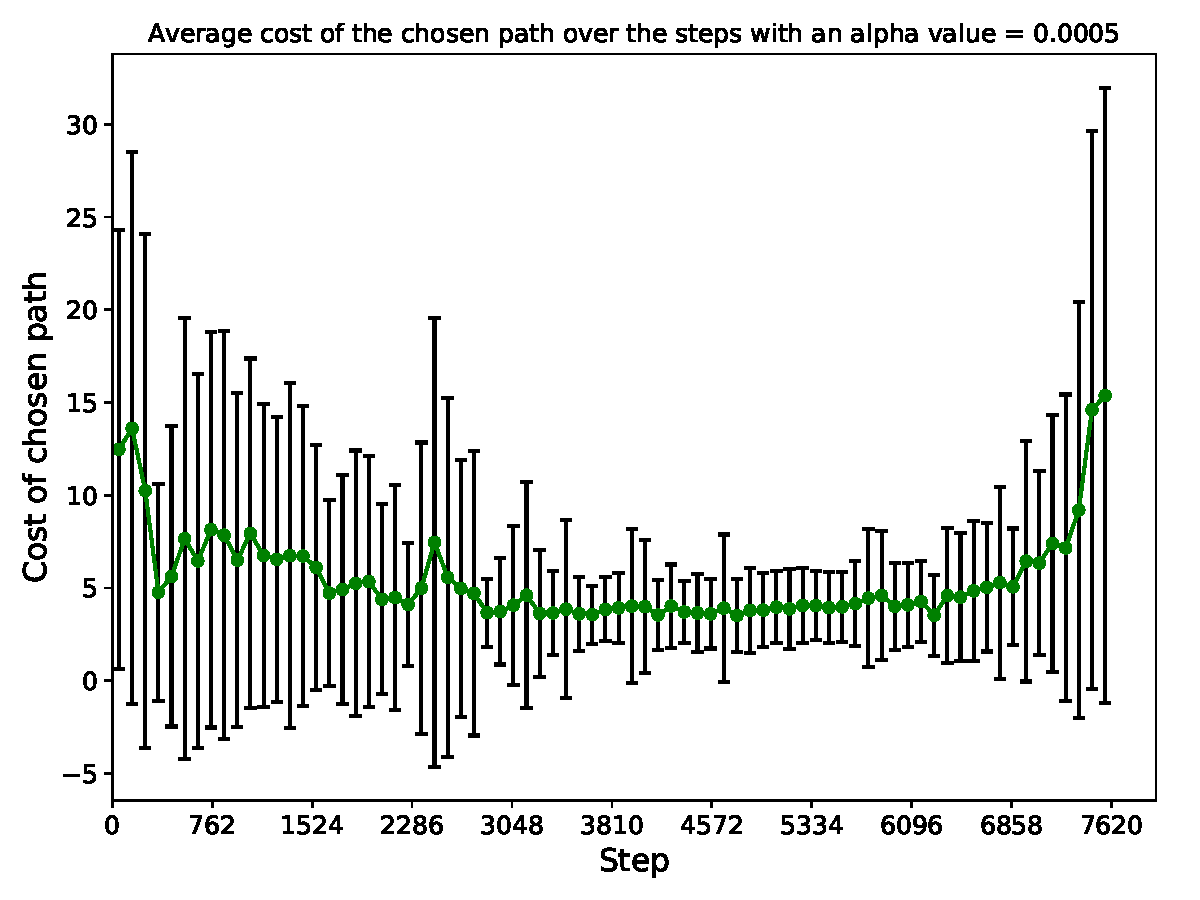
\includegraphics[width = .5\textwidth]{images/alpha_results/cost_alpha_0_0005}}\\
		\subfloat[Effetto di un valore del parametro $\alpha$ pari a 0.001 nella scelta della cella obiettivo in base al costo del cammino.]{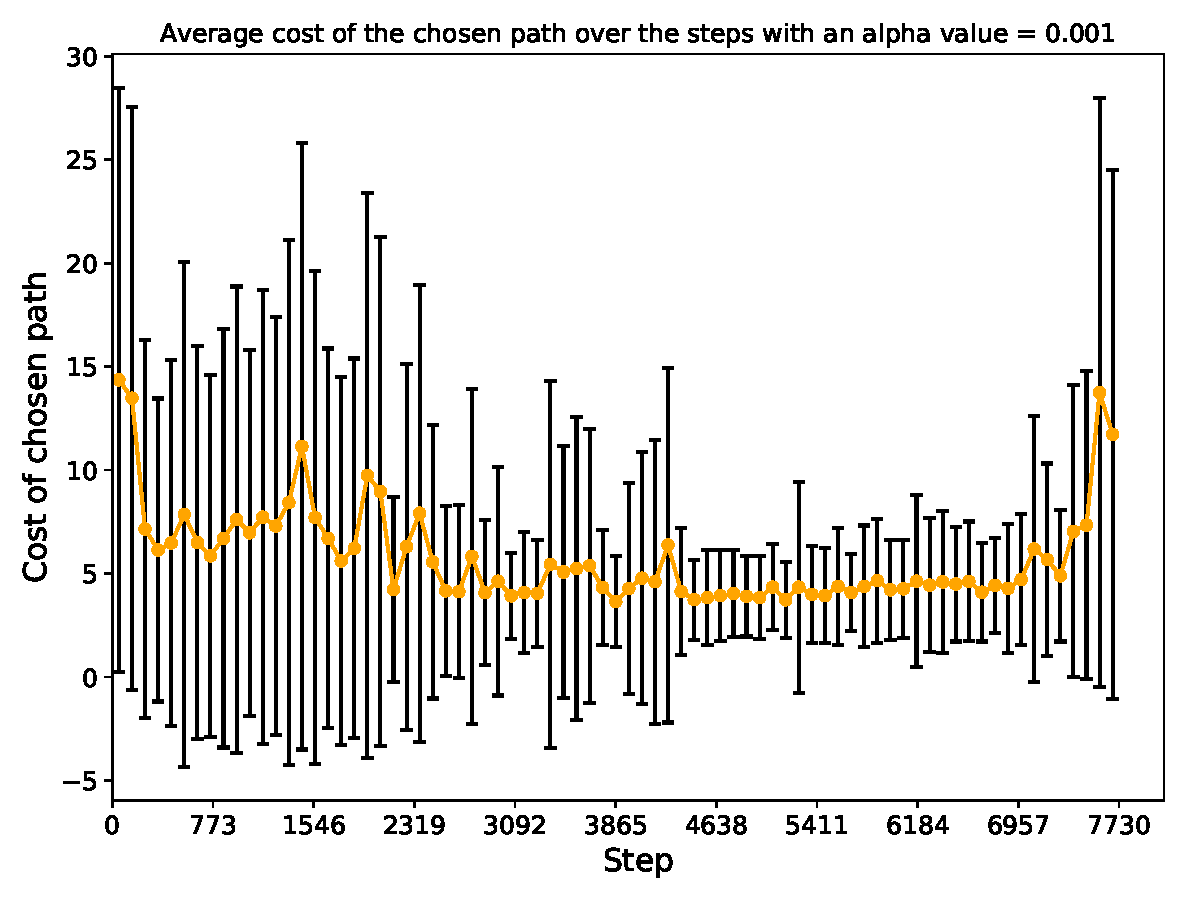
\includegraphics[width = .5\textwidth]{images/alpha_results/cost_alpha_0_001}} &
		\subfloat[Effetto di un valore del parametro $\alpha$ pari a 0.005 nella scelta della cella obiettivo in base al costo del cammino.]{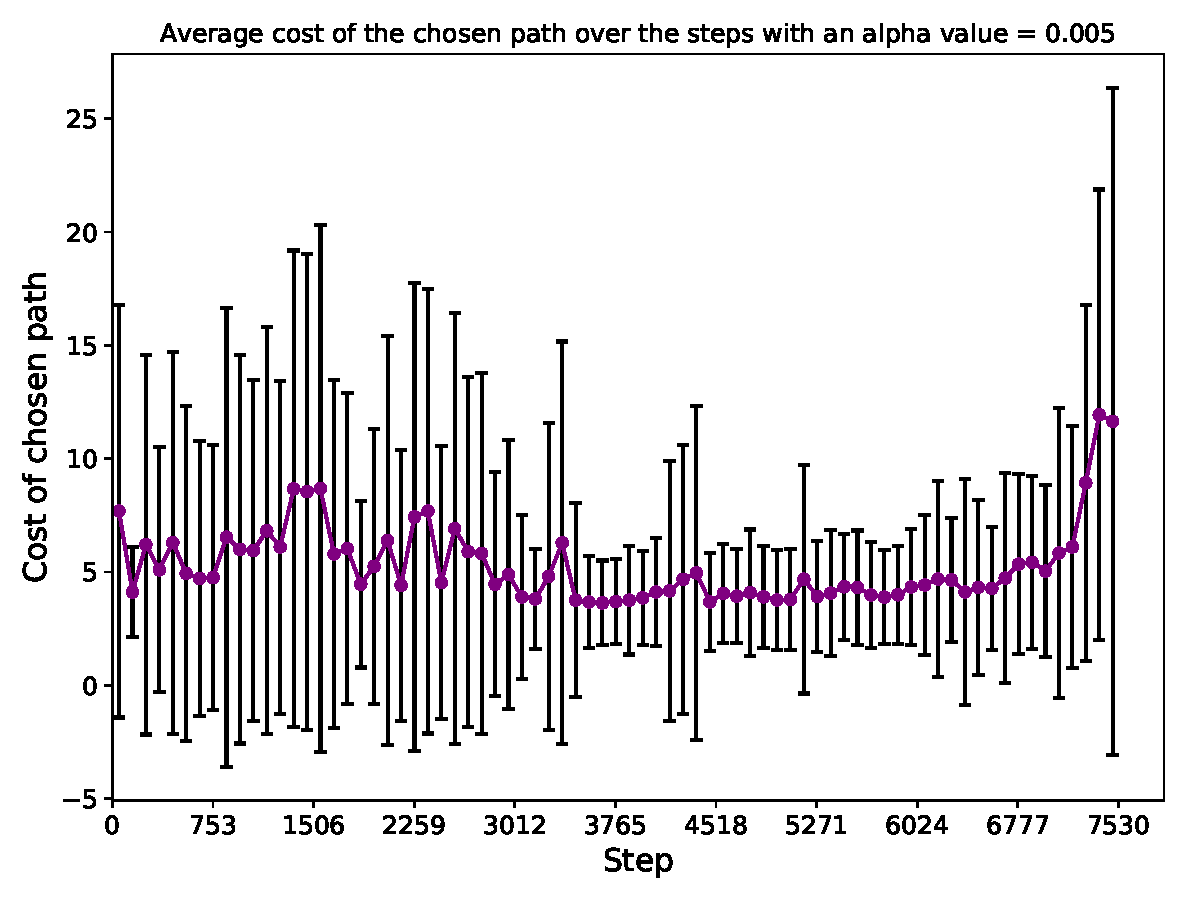
\includegraphics[width = .5\textwidth]{images/alpha_results/cost_alpha_0_005}}\\
	\end{tabular}
	\caption{In colore si denota la media dei costi dei cammini per raggiungere la cella scelta, i valori sono stati calcolati aggregando le scelte effettuate durante intervalli di 100 \textit{step}; in nero gli \textit{errorbar} relativi alla media determinati dalla deviazione standard.}
	\label{figapx:alpha1}
\end{figure}

\begin{figure}
	\begin{tabular}{cc}
		\subfloat[Effetto di un valore del parametro $\alpha$ pari a 0.05 nella scelta della cella obiettivo in base al costo del cammino.\label{sfig:alpha0.05}]{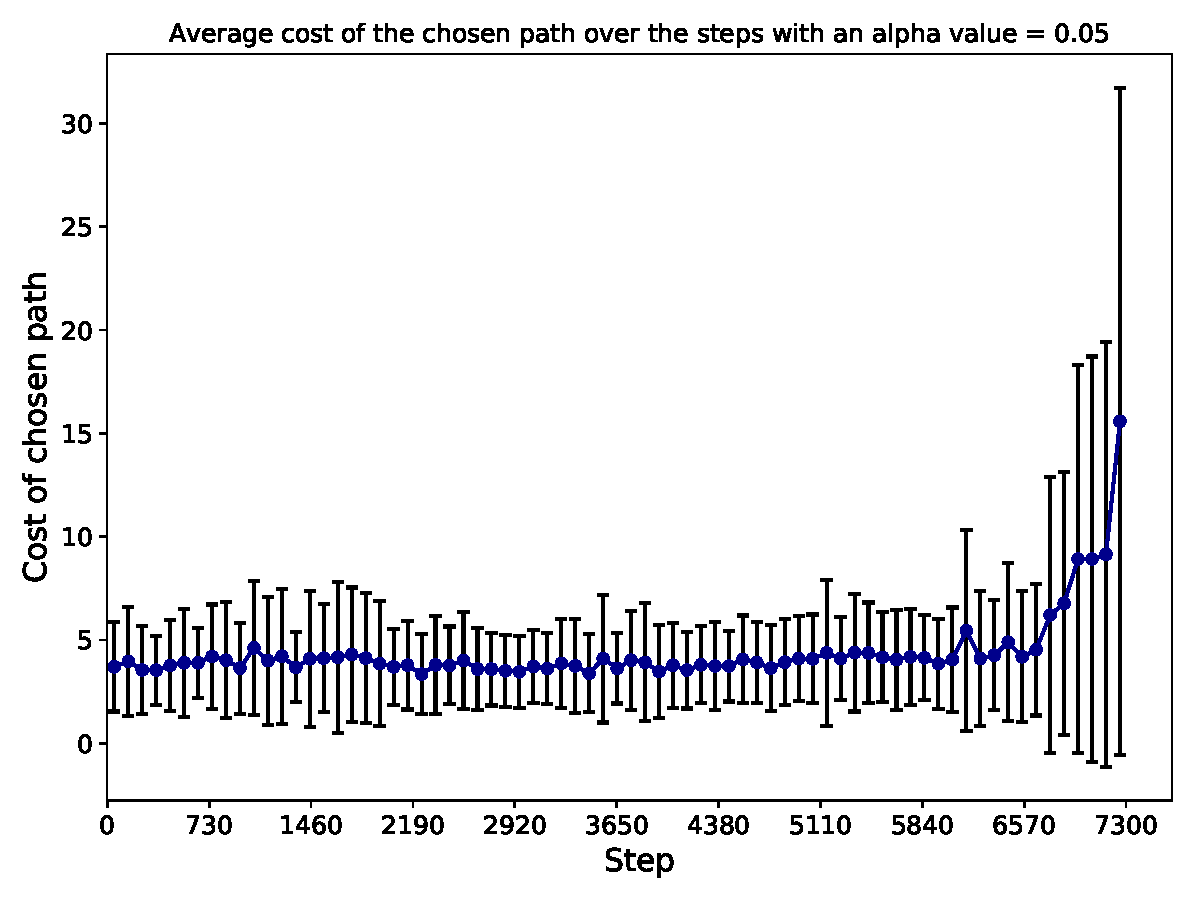
\includegraphics[width = .5\textwidth]{images/alpha_results/cost_alpha_0_05}} &
		\subfloat[Effetto di un valore del parametro $\alpha$ pari a 0.1 nella scelta della cella obiettivo in base al costo del cammino.]{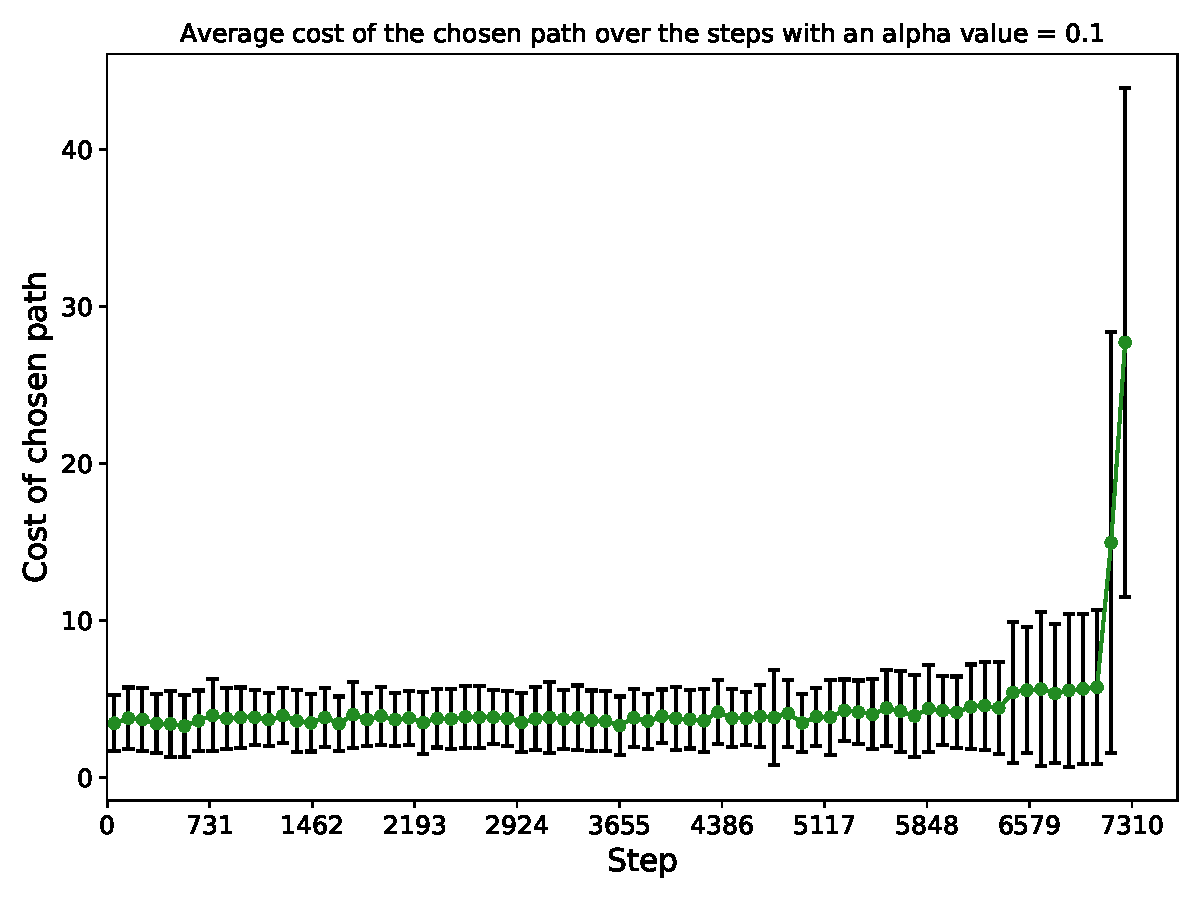
\includegraphics[width = .5\textwidth]{images/alpha_results/cost_alpha_0_1}}\\
	\end{tabular}
		\centering
		\subfloat[Effetto di un valore del parametro $\alpha$ pari a 1 nella scelta della cella obiettivo in base al costo del cammino.]{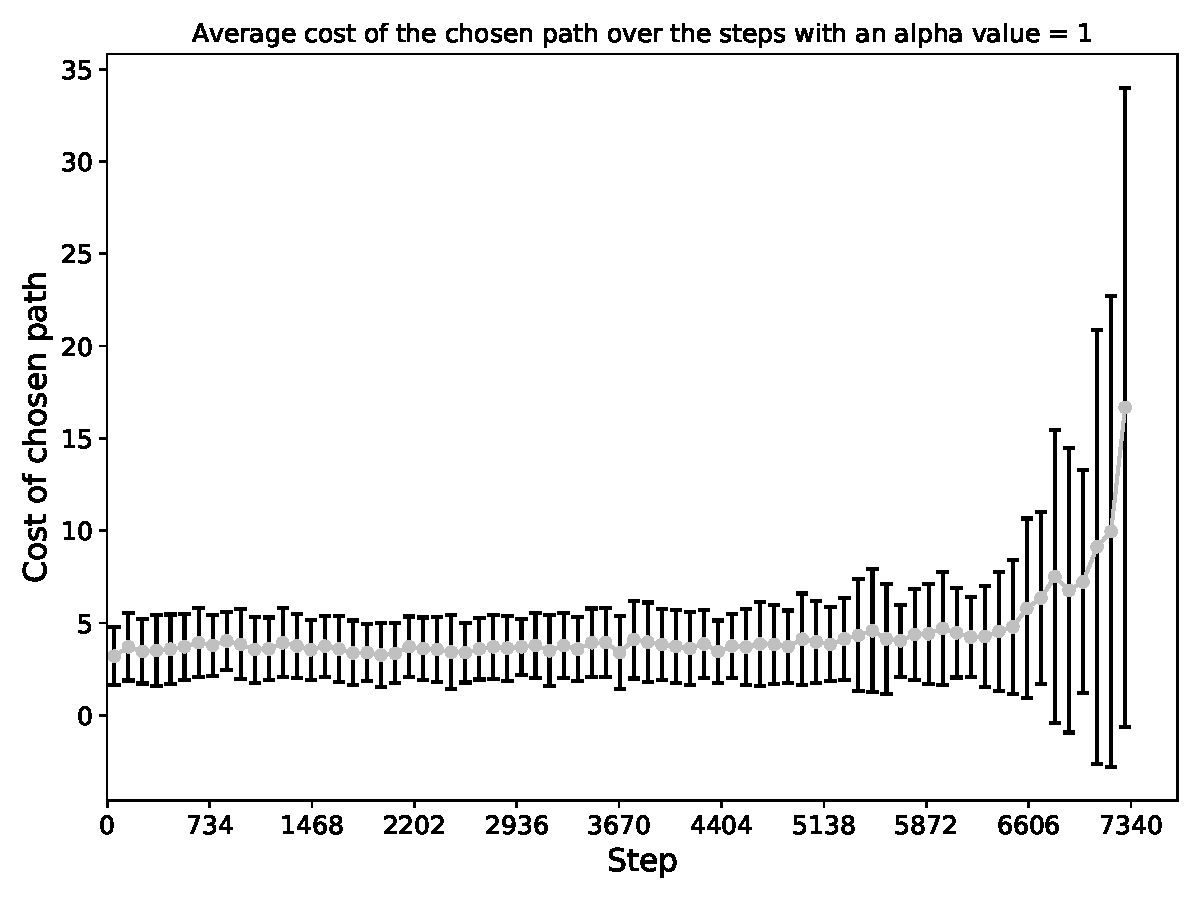
\includegraphics[width = .5\textwidth]{images/alpha_results/cost_alpha_1}}
	\caption{In colore si denota la media dei costi dei cammini per raggiungere la cella scelta, i valori sono stati calcolati aggregando le scelte effettuate durante intervalli di 100 \textit{step}; in nero gli \textit{errorbar} relativi alla media determinati dalla deviazione standard.}
	\label{figapx:alpha2}
\end{figure}
	\chapter{Ulteriori risultati ottenuti dall'analisi del parametro $\gamma$}
	\label{apx:gamma}
	\section{Ulteriori grafici derivanti dalle analisi con valore di $\alpha$ basso}
Nel seguente appendice, si mostrano brevemente i grafici che non sono stati inseriti direttamente nel Sezione \ref{sec:gamma}, dove sono stati discussi gli effetti che ha il parametro $\gamma$ rispetto alla distanza media che mantengono gli agenti durante l'esplorazione.

In Figura \ref{figapx:gammavsdistance}, si mostra come varia la media, calcolata su dieci simulazioni, delle distanze medie durante le simulazioni per ogni valore di $\gamma$, la media delle relative deviazioni standard e la deviazione standard massima ottenuta durante una simulazione. 
Poiché tale grafico aggrega molti dati insieme non è stato considerato significativo riportarlo nel Capitolo \ref{chap:results}.\\
\begin{figure}
	\centering
	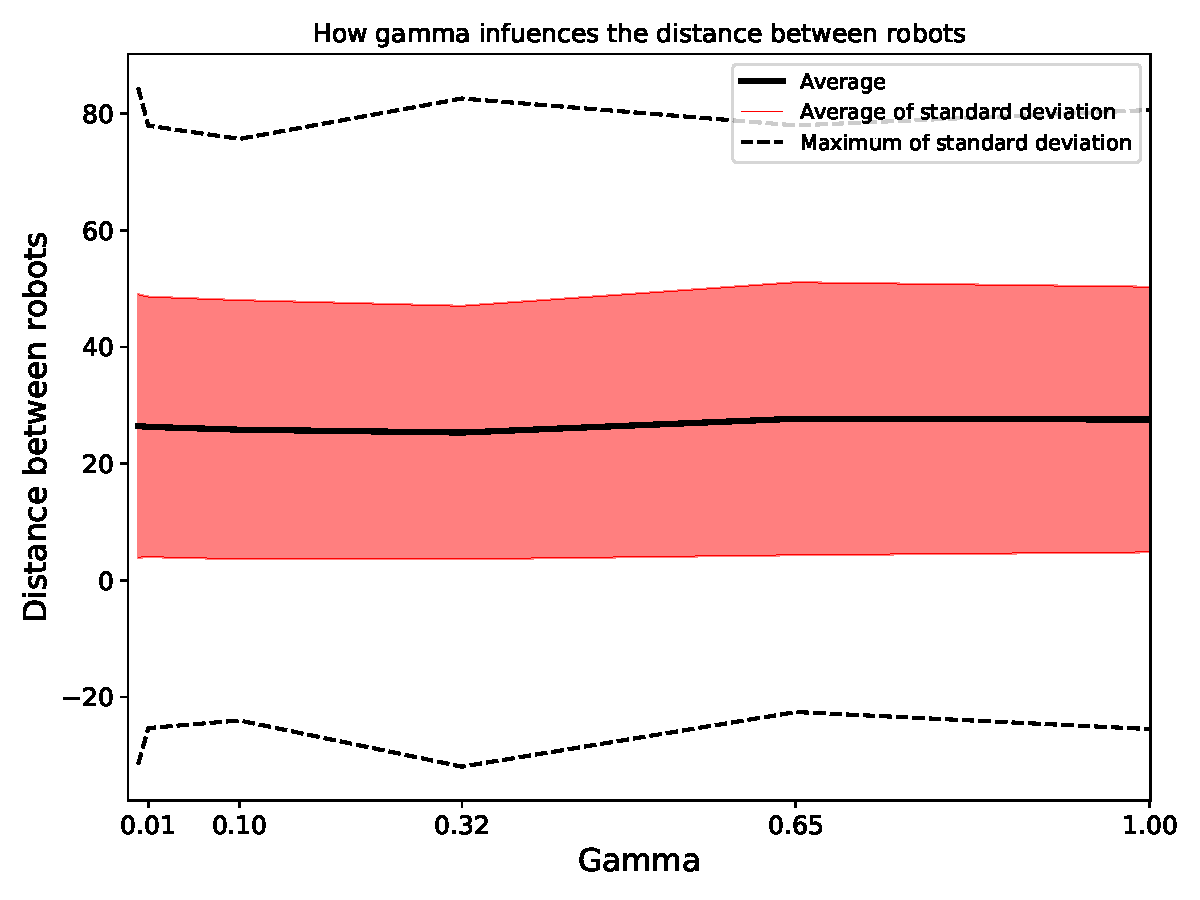
\includegraphics[width=0.9\linewidth]{images/gamma_results/low_alpha/gamma_vs_distance}
	\caption{In nero è rappresentata la media delle distanze medie mantenute durante le dieci simulazioni per ogni valore di $\gamma$, la media delle diaviozni standard calcolate per ogni simulazione e infine la riga tratteggiata rappresenta il valore massimo di deviazione standard ottenuto per ogni valore di $\gamma$.}
	\label{figapx:gammavsdistance}
\end{figure}
In Figura \ref{figapx:gammaDistr} sono mostrate le distribuzioni delle distanze medie tra gli agenti durante le simulazioni per ogni valore di $\gamma$ analizzato, in aggiunta a quelle mostrate nella Sotto-sezione \ref{subsec:gammaalow}.\\
\begin{figure}
	\begin{tabular}{cc}
		\subfloat[Distribuzione della distanza media mantenuta dai robot con un valore di $\gamma$ pari a 0.]{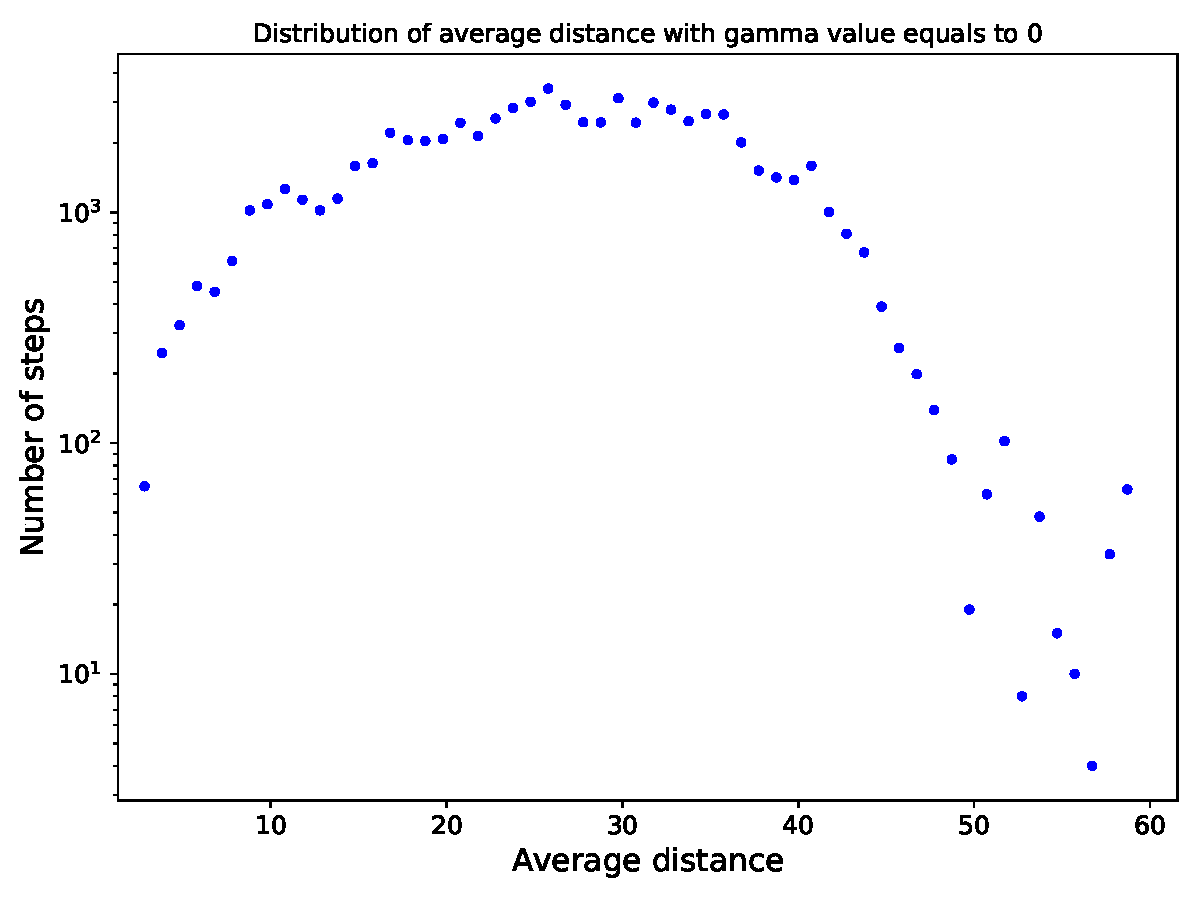
\includegraphics[width = .5\textwidth]{images/gamma_results/low_alpha/distribution_distance_gamma_0}} &
		\subfloat[Distribuzione della distanza media mantenuta dai robot con un valore di $\gamma$ pari a 0.01.]{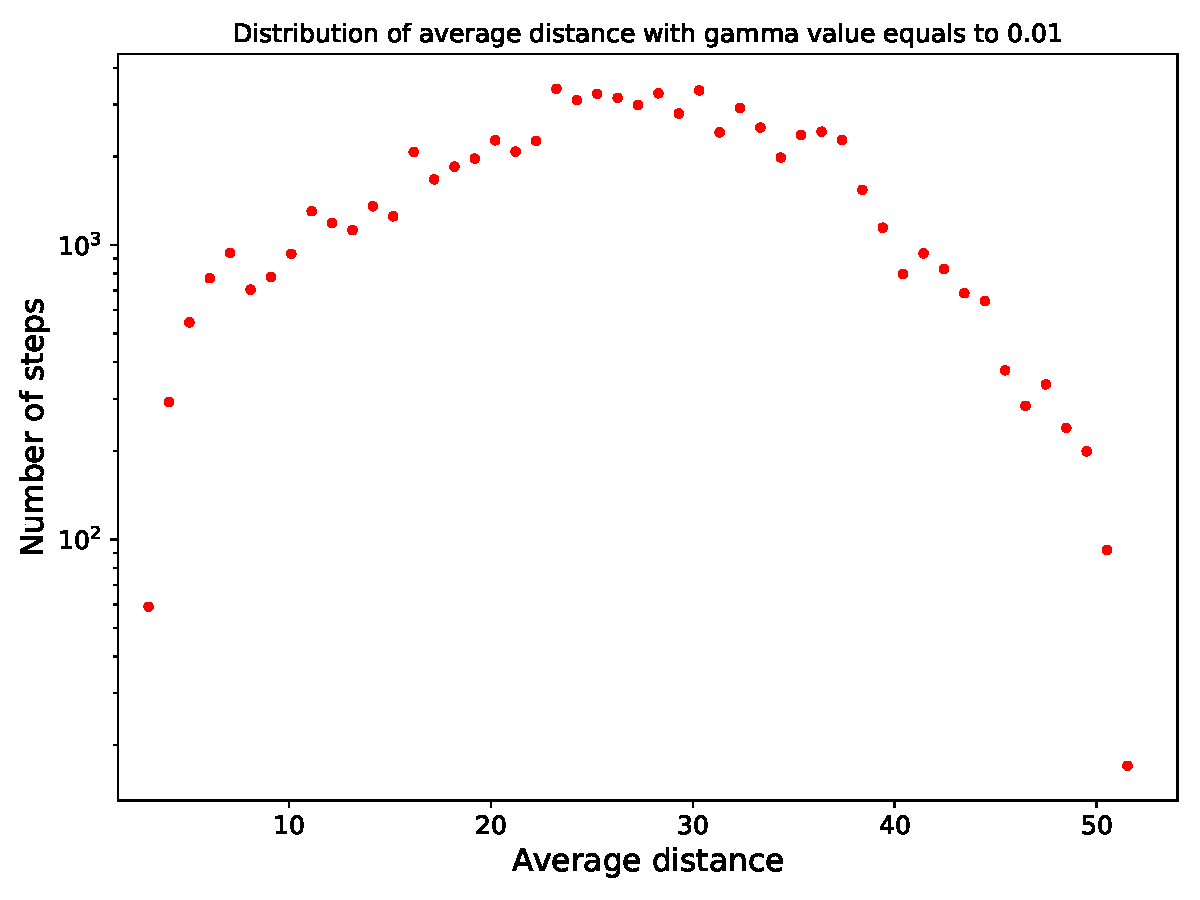
\includegraphics[width = .5\textwidth]{images/gamma_results/low_alpha/distribution_distance_gamma_0_01}}\\
		\subfloat[Distribuzione della distanza media mantenuta dai robot con un valore di $\gamma$ pari a 0.1.]{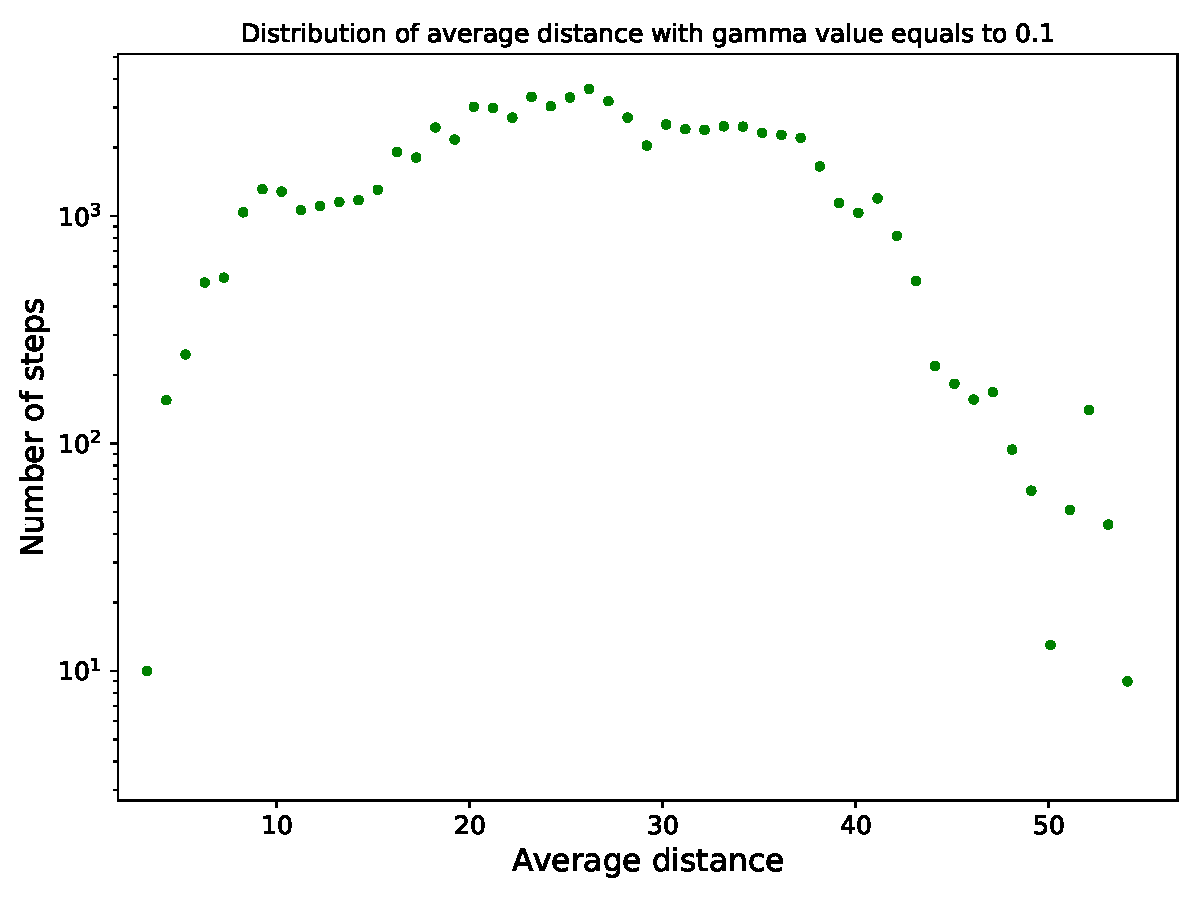
\includegraphics[width = .5\textwidth]{images/gamma_results/low_alpha/distribution_distance_gamma_0_1}} &
		\subfloat[Distribuzione della distanza media mantenuta dai robot con un valore di $\gamma$ pari a 1.]{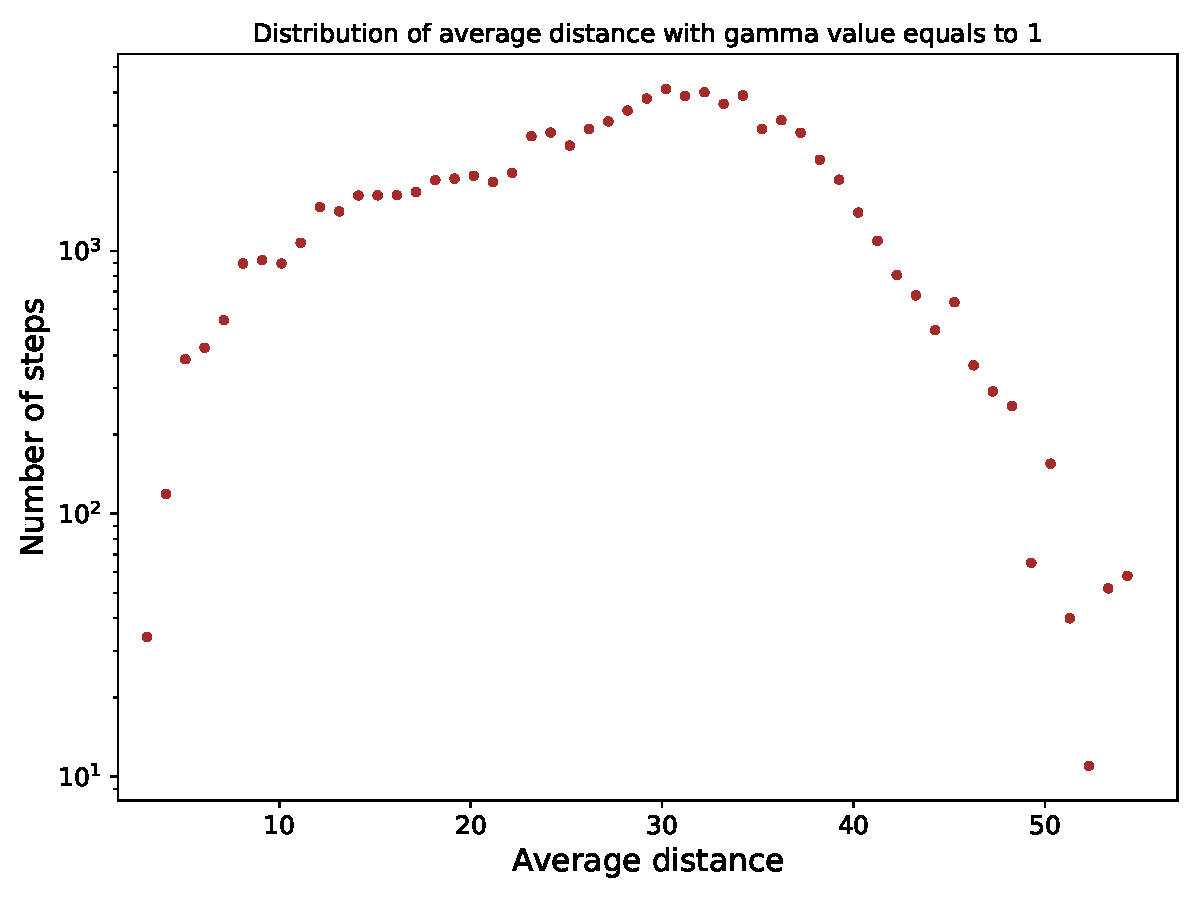
\includegraphics[width = .5\textwidth]{images/gamma_results/low_alpha/distribution_distance_gamma_1}}\\
	\end{tabular}
	\caption{Distribuzione della distanza media mantenuta dai robot al variare del valore di $\gamma$, per valutare la distribuzione si è conteggiato in quanti \textit{step} i robot hanno presentato tale distanza, il numero di \textit{bin} per produrre la distribuzione è pari alla differenza tra la distanza minima e massima presente durante la simulazione, tale valore è stato poi arrotondato. Infine si noti che l'asse delle \textit{y} è a scala logaritmica.}
	\label{figapx:gammaDistr}
\end{figure}
In Figura \ref{figapx:gammaSim} sono rappresentate le distanze medie e deviazioni standard per ogni \textit{step} di una simulazione, la simulazione è stata scelta casualmente tra le dieci effettuate per la raccolta dei dati.
\begin{figure}
	\begin{tabular}{cc}
		\subfloat[Evoluzione della distanza media tra gli agenti con un valore di $\gamma$ pari a 0.]{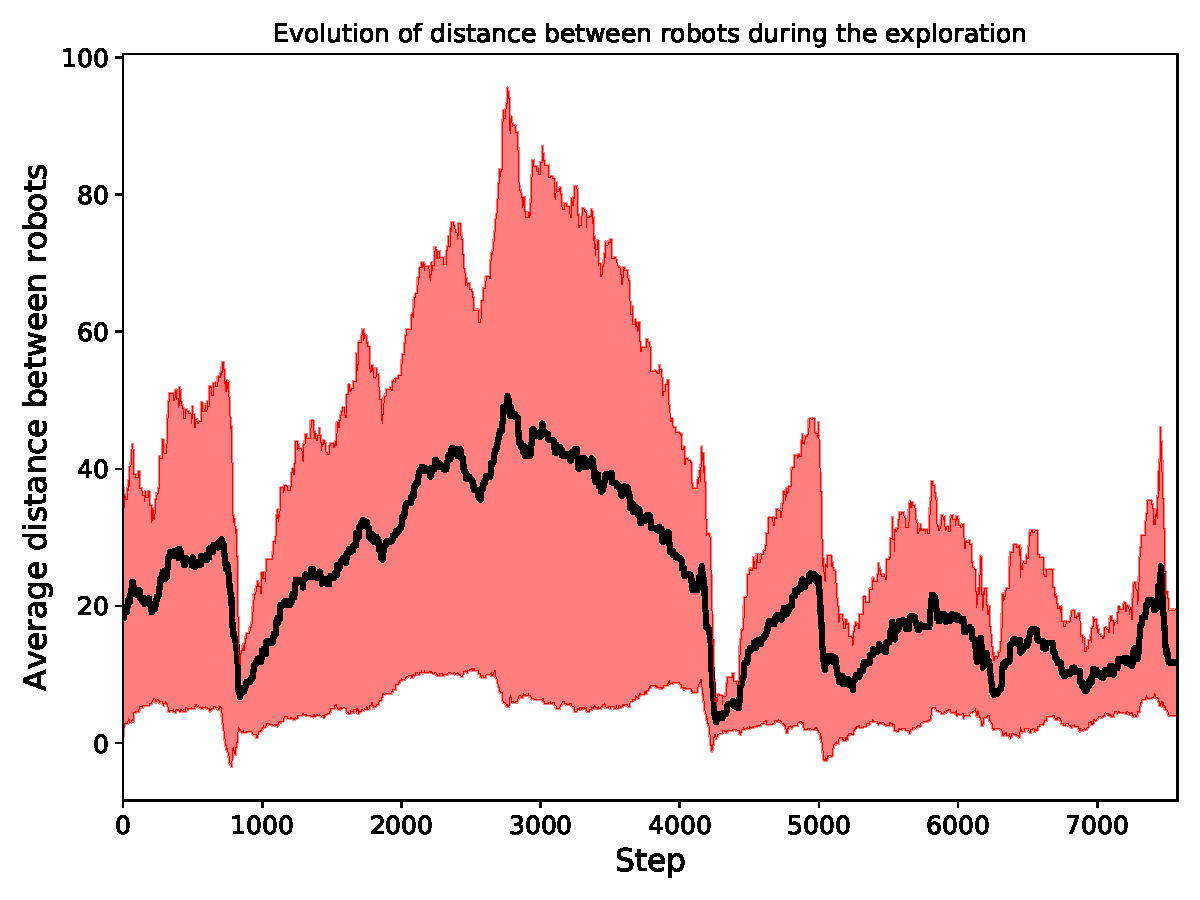
\includegraphics[width = .5\textwidth]{images/gamma_results/low_alpha/dinstance_simulation_gamma_0_simid_0}} &
		\subfloat[Evoluzione della distanza media tra gli agenti con un valore di $\gamma$ pari a 0.01.]{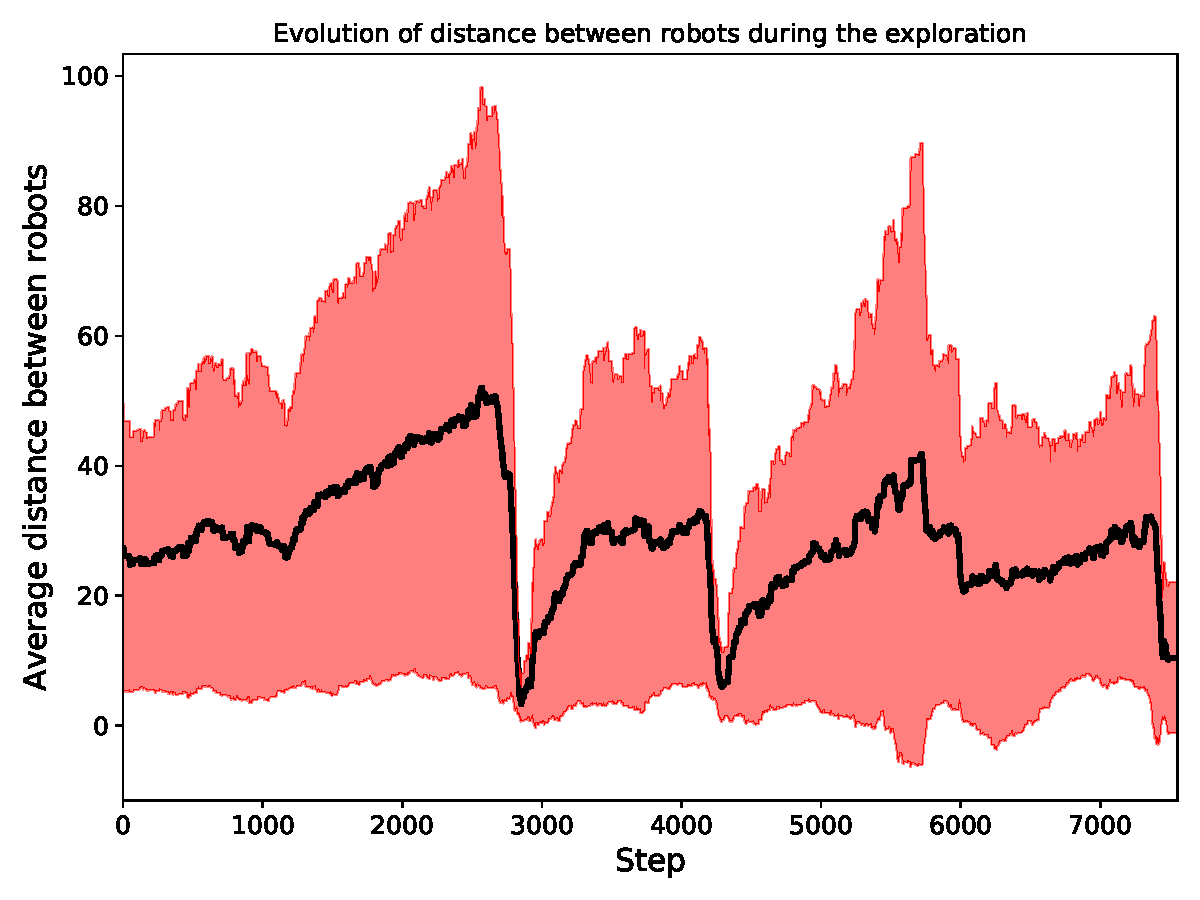
\includegraphics[width = .5\textwidth]{images/gamma_results/low_alpha/dinstance_simulation_gamma_0_01_simid_6}}\\
		\subfloat[Evoluzione della distanza media tra gli agenti con un valore di $\gamma$ pari a 0.1.]{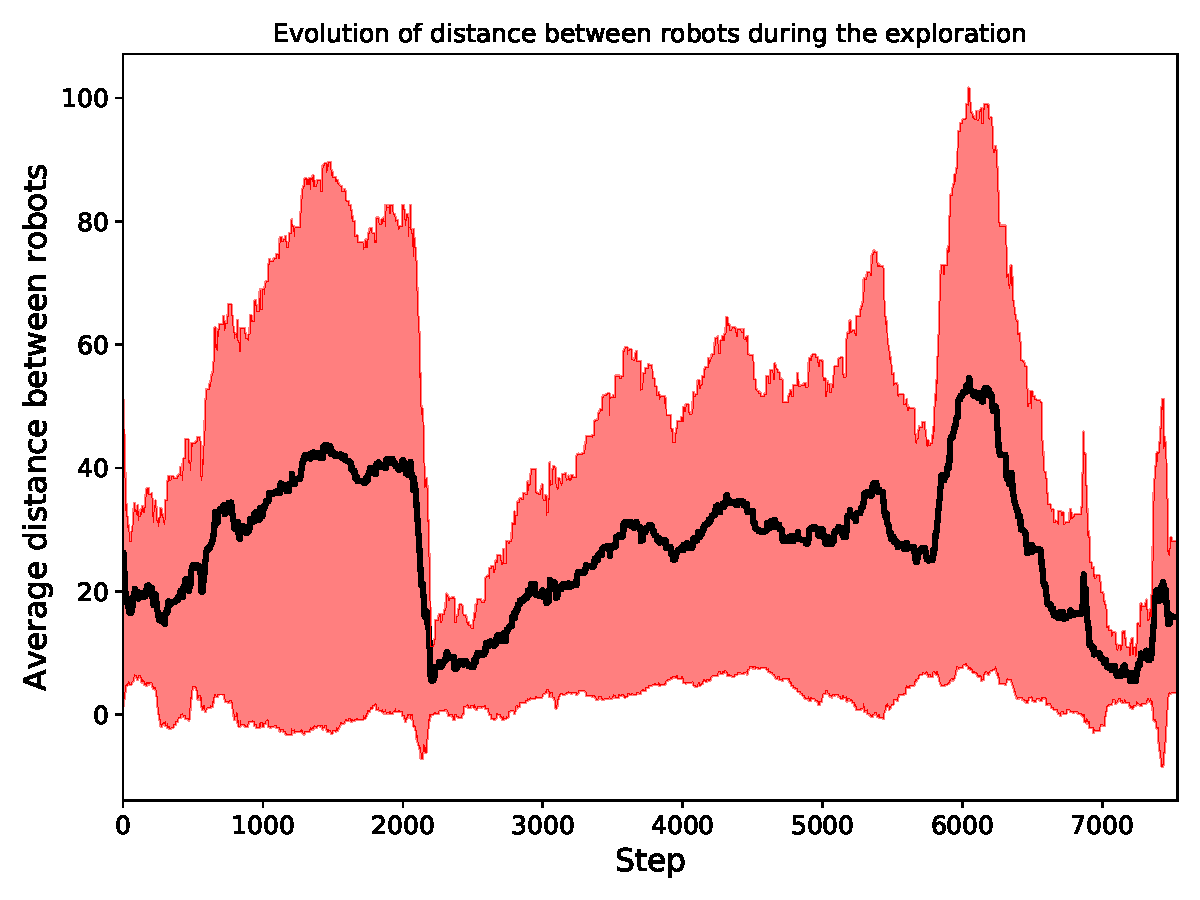
\includegraphics[width = .5\textwidth]{images/gamma_results/low_alpha/dinstance_simulation_gamma_0_1_simid_0}} &
		\subfloat[Evoluzione della distanza media tra gli agenti con un valore di $\gamma$ pari a 1.]{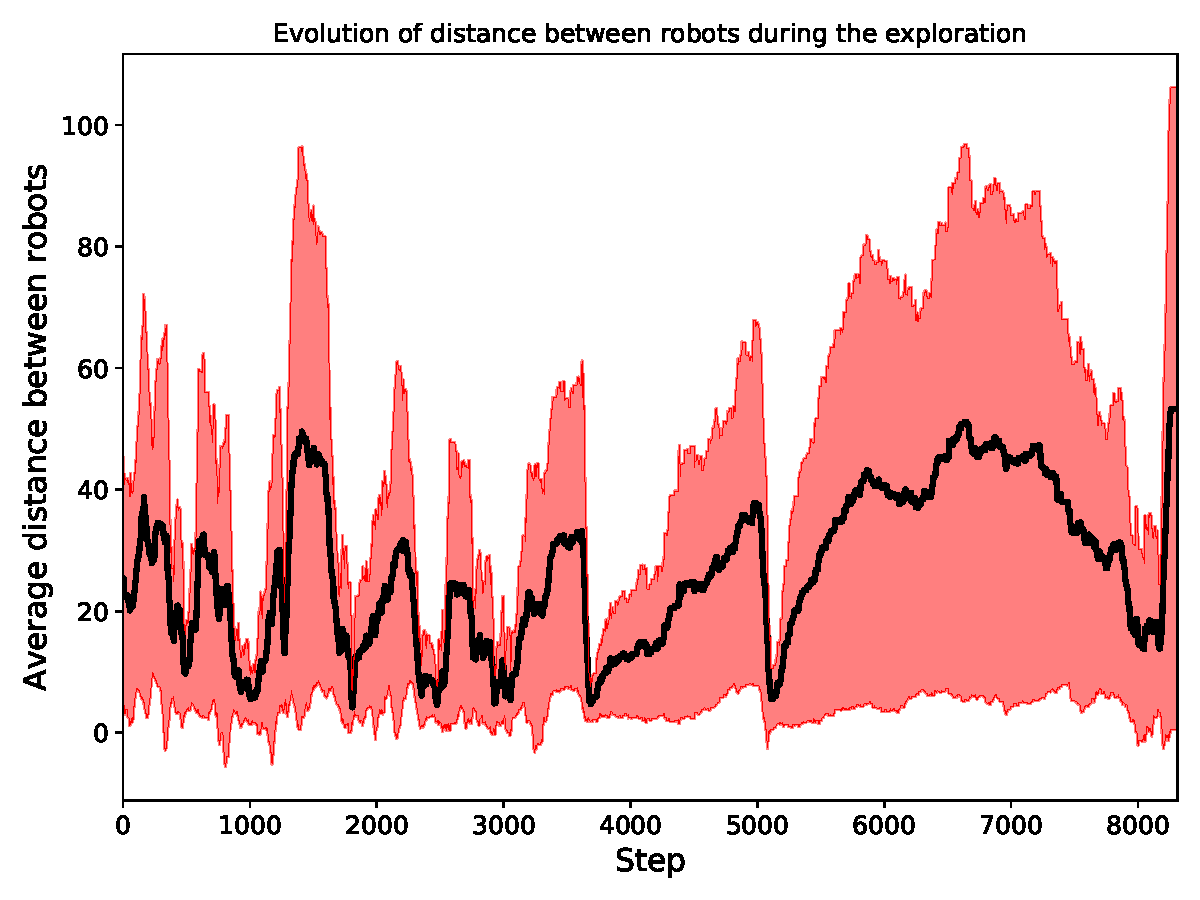
\includegraphics[width = .5\textwidth]{images/gamma_results/low_alpha/dinstance_simulation_gamma_1_simid_5}}\\
	\end{tabular}
	\caption{Sull'asse delle \textit{x} si trova il tempo, in termini di \textit{step}, impiegato per l'esplorazione della mappa, mentre sull'asse delle \textit{y} la distanza media tra gli agenti.}
	\label{figapx:gammaSim}
\end{figure}
\clearpage
\section{Ulteriori grafici derivanti dalle analisi con valore di $\alpha$ elevato}
Come in precedenza, in Figura \ref{figapx:gammavsdistanceH}, si mostra come varia la media, calcolata su dieci simulazioni, delle distanze medie durante le simulazioni per ogni valore di $\gamma$, la media delle relative deviazioni standard e la deviazione standard massima ottenuta durante una simulazione.
\begin{figure}
	\centering
	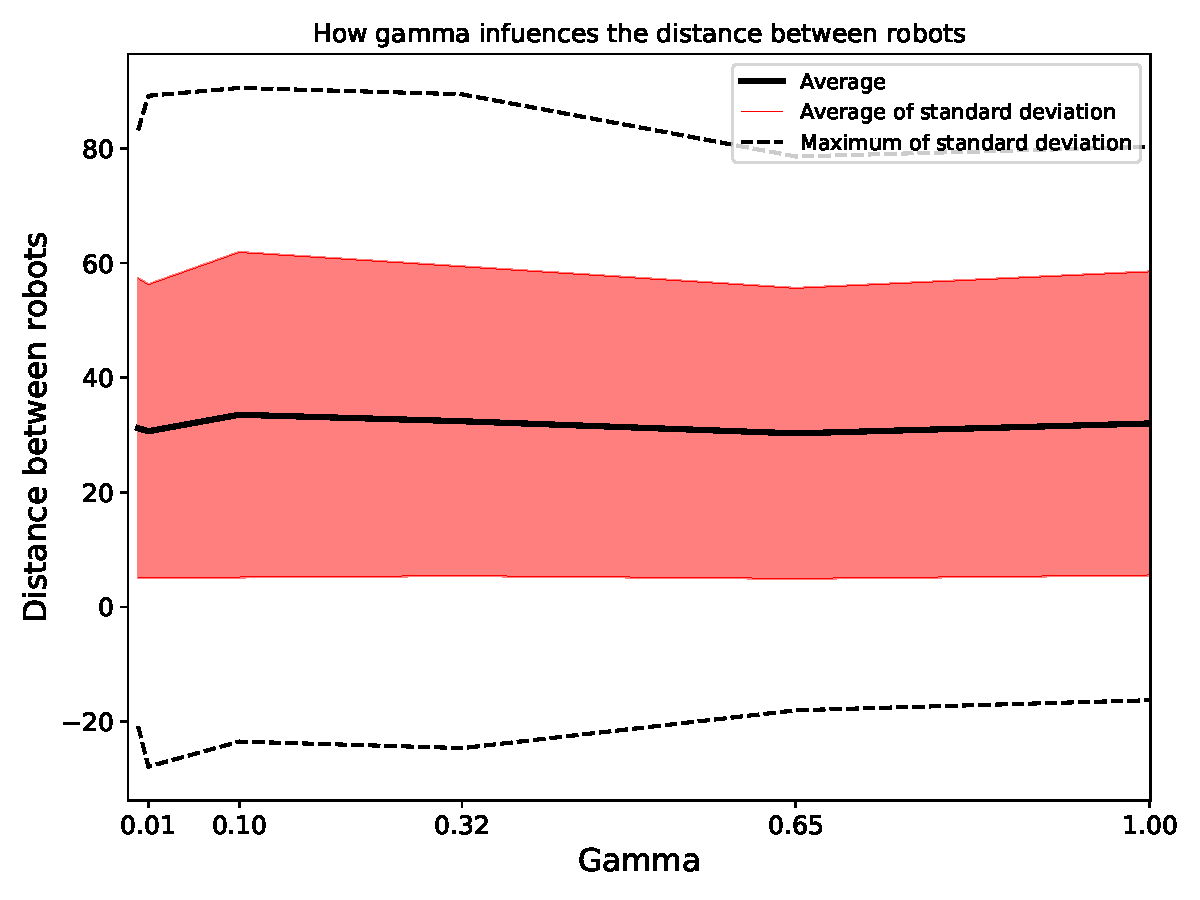
\includegraphics[width=0.9\linewidth]{images/gamma_results/high_alpha/gamma_vs_distance}
	\caption{In nero è rappresentata la media delle distanze medie mantenute durante le dieci simulazioni per ogni valore di $\gamma$, la media delle diaviozni standard calcolate per ogni simulazione e infine la riga tratteggiata rappresenta il valore massimo di deviazione standard ottenuto per ogni valore di $\gamma$.}
	\label{figapx:gammavsdistanceH}
\end{figure}
In Figura \ref{figapx:gammaHDistr} sono mostrate le distribuzioni delle distanze medie tra gli agenti durante le simulazioni per ogni valore di $\gamma$ analizzato, in aggiunta a quelle mostrate nella Sotto-sezione \ref{subsec:gammaahigh}.\\
\begin{figure}
	\begin{tabular}{cc}
		\subfloat[Distribuzione della distanza media mantenuta dai robot con un valore di $\gamma$ pari a 0.]{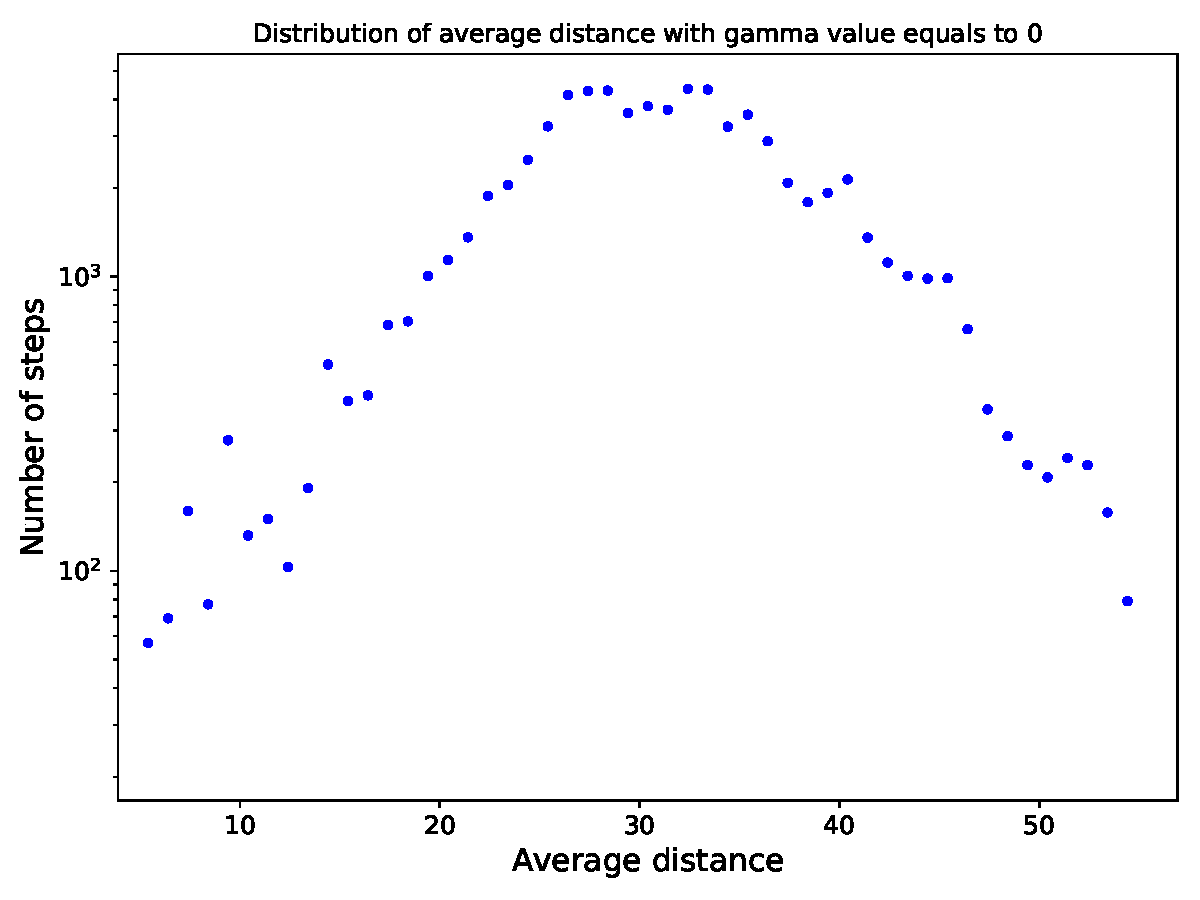
\includegraphics[width = .5\textwidth]{images/gamma_results/high_alpha/distribution_distance_gamma_0}} &
		\subfloat[Distribuzione della distanza media mantenuta dai robot con un valore di $\gamma$ pari a 0.01.]{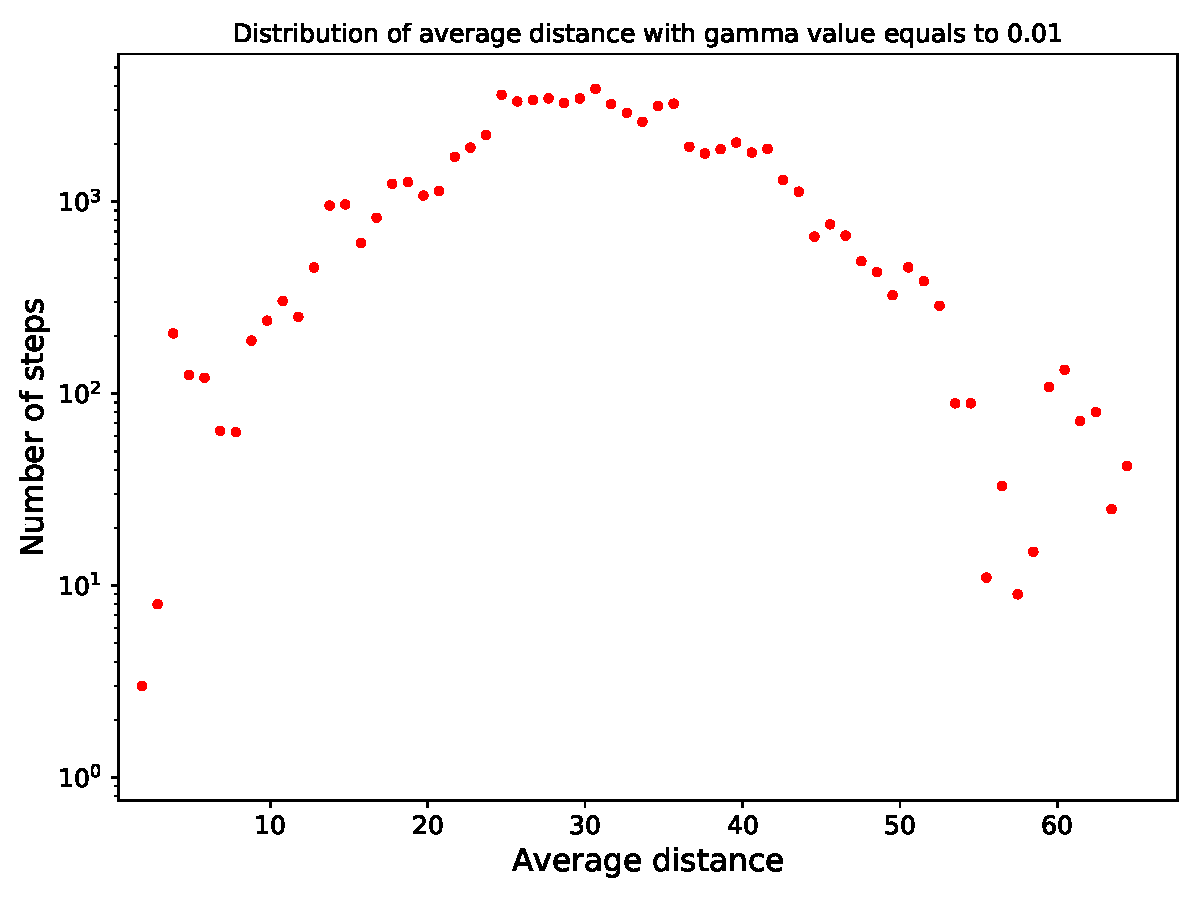
\includegraphics[width = .5\textwidth]{images/gamma_results/high_alpha/distribution_distance_gamma_0_01}}\\
		\subfloat[Distribuzione della distanza media mantenuta dai robot con un valore di $\gamma$ pari a 0.1.]{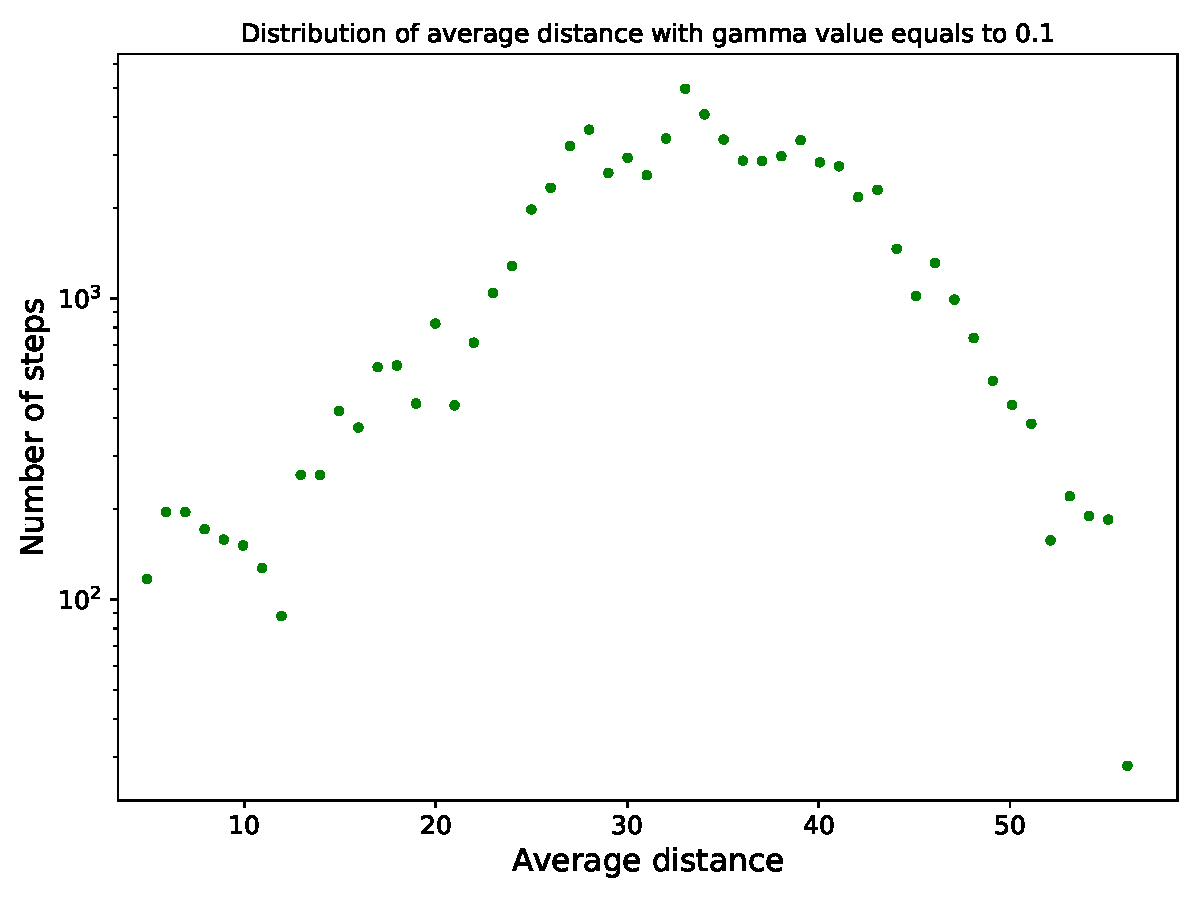
\includegraphics[width = .5\textwidth]{images/gamma_results/high_alpha/distribution_distance_gamma_0_1}} &
		\subfloat[Distribuzione della distanza media mantenuta dai robot con un valore di $\gamma$ pari a 1.]{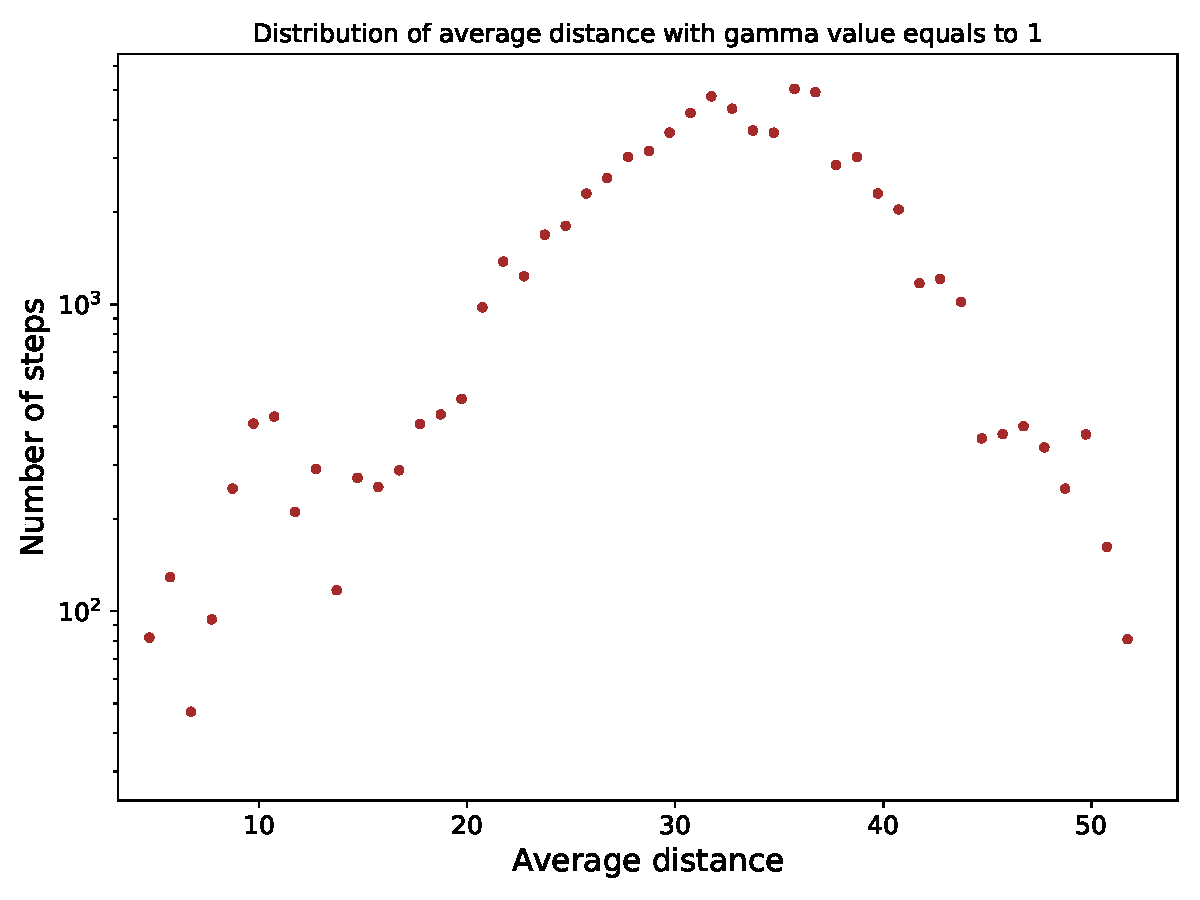
\includegraphics[width = .5\textwidth]{images/gamma_results/high_alpha/distribution_distance_gamma_1}}\\
	\end{tabular}
	\caption{Distribuzione della distanza media mantenuta dai robot al variare del valore di $\gamma$, per valutare la distribuzione si è conteggiato in quanti \textit{step} i robot hanno presentato tale distanza, il numero di \textit{bin} per produrre la distribuzione è pari alla differenza tra la distanza minima e massima presente durante la simulazione, tale valore è stato poi arrotondato. Infine si noti che l'asse delle \textit{y} è a scala logaritmica.}
	\label{figapx:gammaHDistr}
\end{figure}
In Figura \ref{figapx:gammaHSim} sono rappresentate le distanze medie e deviazioni standard per ogni \textit{step} di una simulazione, la simulazione è stata scelta casualmente tra le dieci effettuate per la raccolta dei dati.
\begin{figure}
	\begin{tabular}{cc}
		\subfloat[Evoluzione della distanza media tra gli agenti con un valore di $\gamma$ pari a 0.]{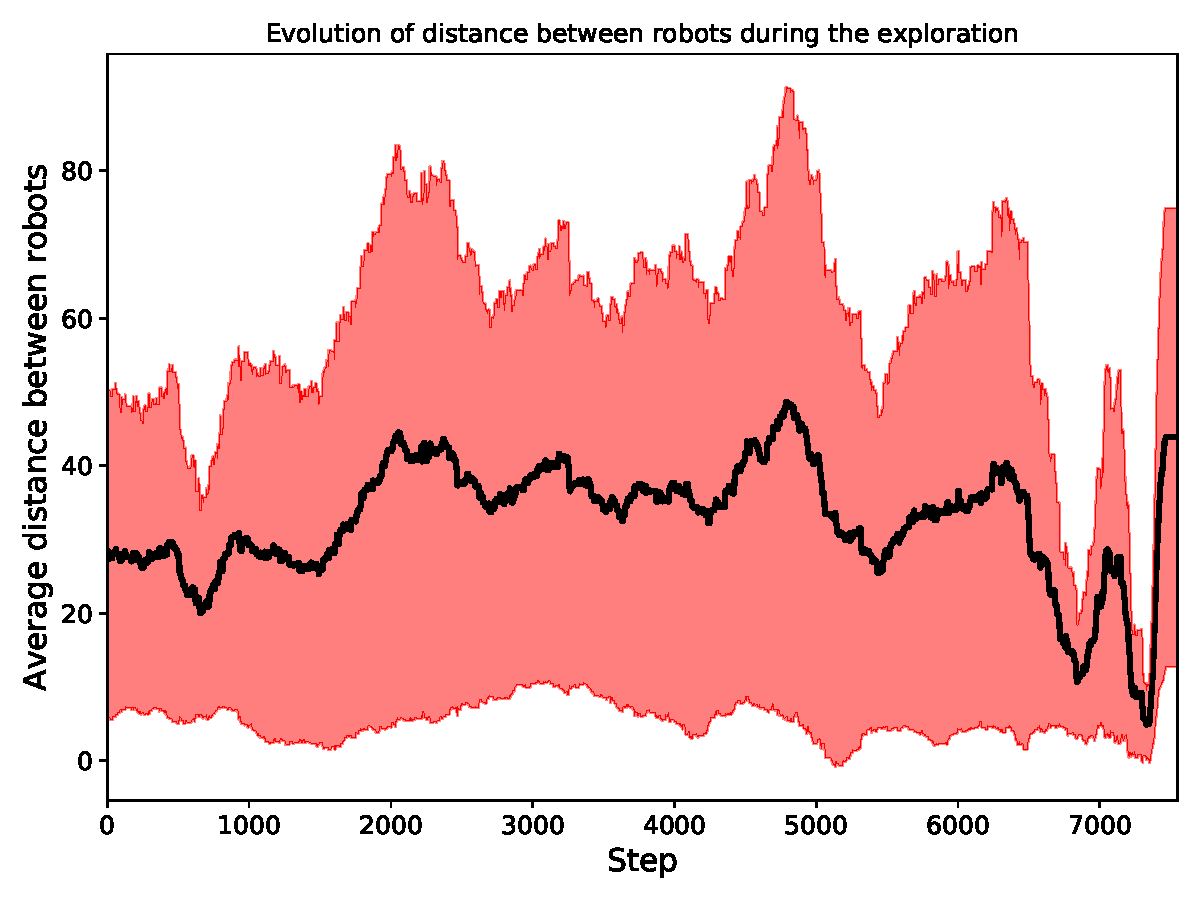
\includegraphics[width = .5\textwidth]{images/gamma_results/high_alpha/dinstance_simulation_gamma_0_simid_9}} &
		\subfloat[Evoluzione della distanza media tra gli agenti con un valore di $\gamma$ pari a 0.01.]{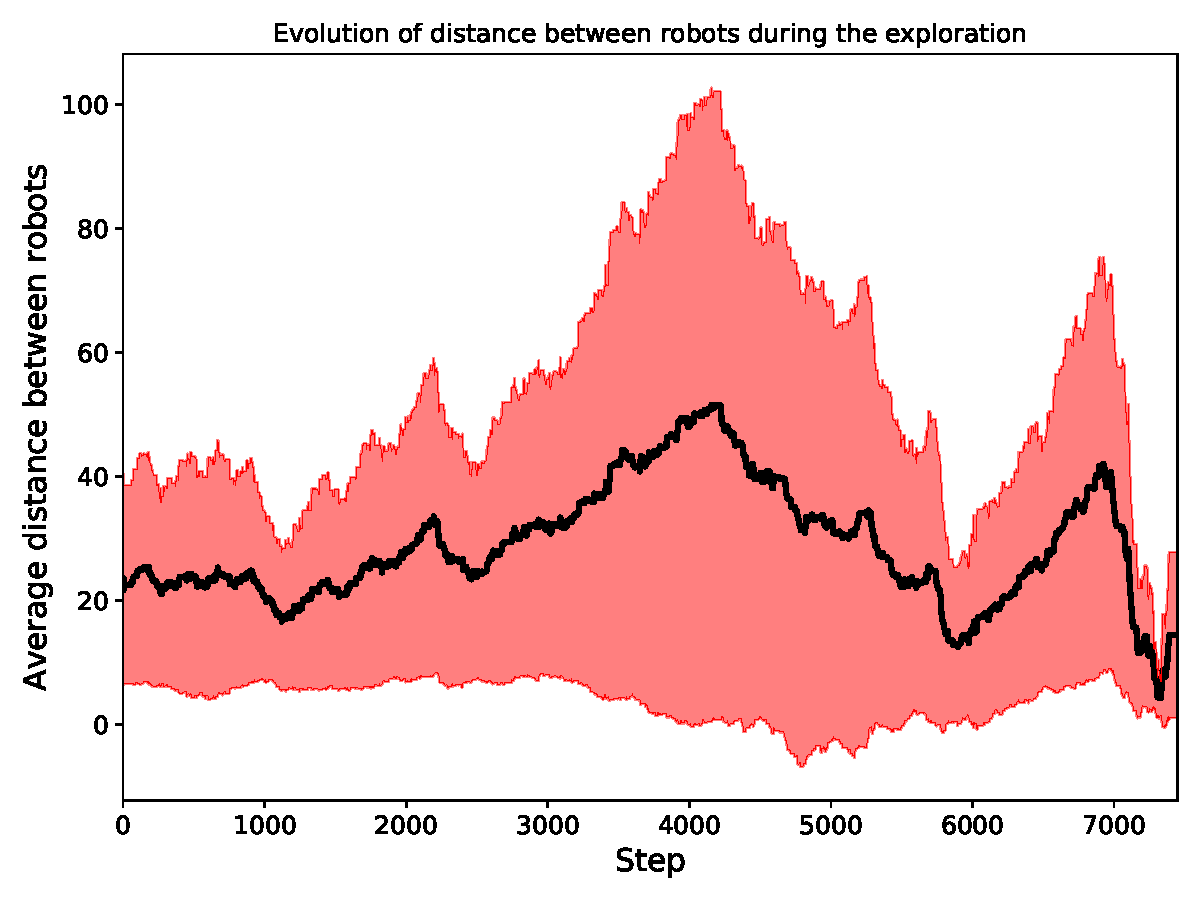
\includegraphics[width = .5\textwidth]{images/gamma_results/high_alpha/dinstance_simulation_gamma_0_01_simid_6}}\\
		\subfloat[Evoluzione della distanza media tra gli agenti con un valore di $\gamma$ pari a 0.1.]{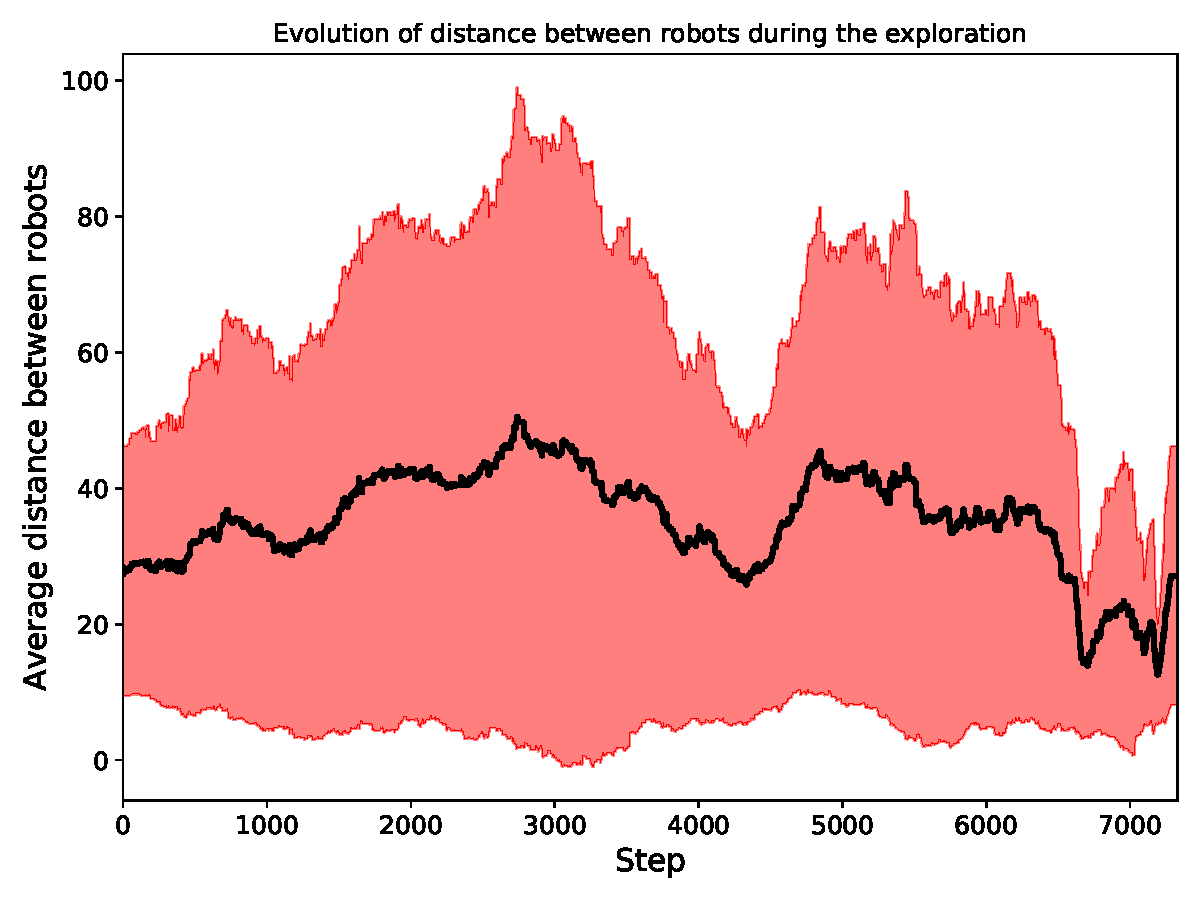
\includegraphics[width = .5\textwidth]{images/gamma_results/high_alpha/dinstance_simulation_gamma_0_1_simid_5}} &
		\subfloat[Evoluzione della distanza media tra gli agenti con un valore di $\gamma$ pari a 1.]{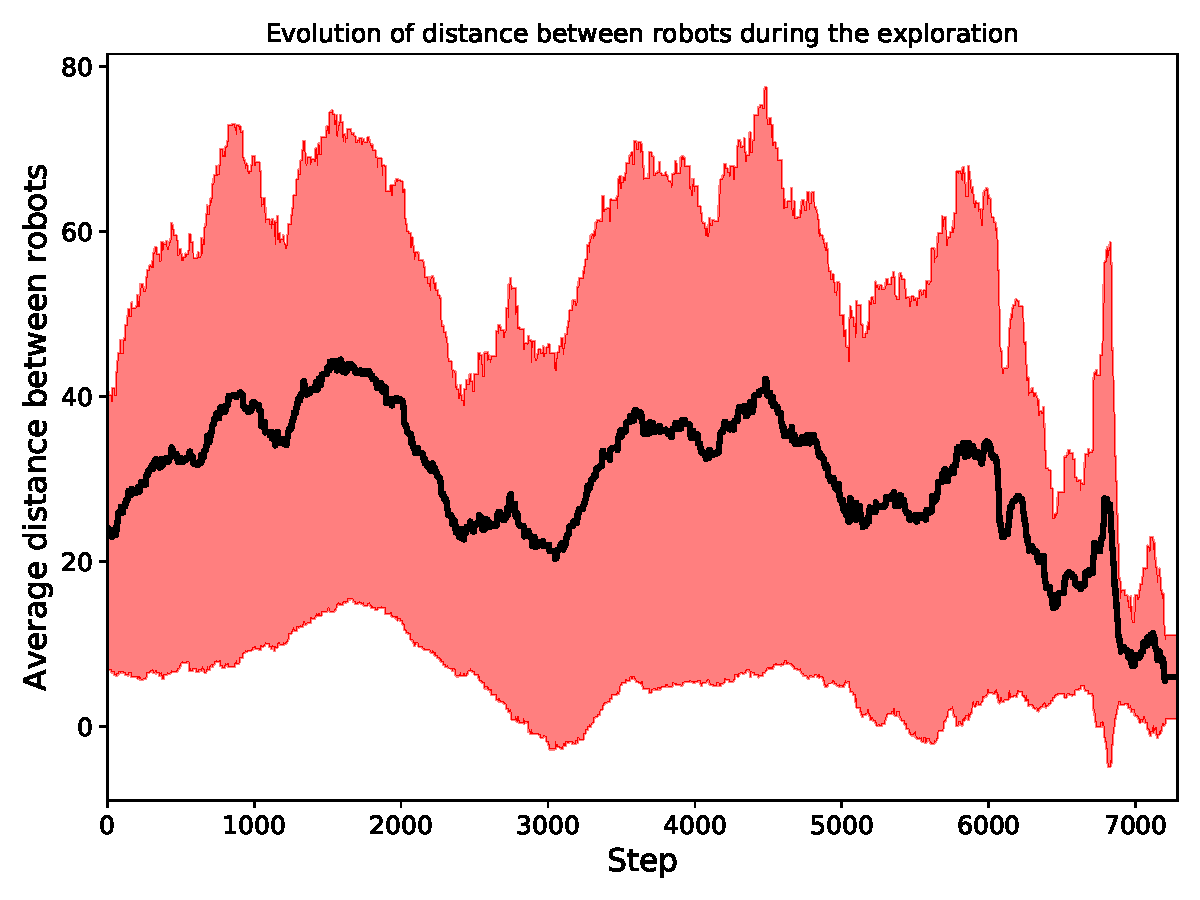
\includegraphics[width = .5\textwidth]{images/gamma_results/high_alpha/dinstance_simulation_gamma_1_simid_3}}\\
	\end{tabular}
	\caption{Sull'asse delle \textit{x} si trova il tempo, in termini di \textit{step}, impiegato per l'esplorazione della mappa, mentre sull'asse delle \textit{y} la distanza media tra gli agenti.}
	\label{figapx:gammaHSim}
\end{figure}
\section{Ulteriori grafici derivanti dalle analisi del metodo di prioritizzazione alternativo}
\subsection{Ulteriori grafici derivanti dalle analisi con valore di $\alpha$ basso}
In Figura \ref{figapx:ngammaLSim} sono rappresentate le distanze medie e deviazioni standard per ogni \textit{step} di una simulazione, la simulazione è stata scelta casualmente tra le dieci effettuate per la raccolta dei dati.
\begin{figure}
	\begin{tabular}{cc}
		\subfloat[Evoluzione della distanza media tra gli agenti con un valore di $\gamma$ pari a 0.]{\includegraphics[width = .5\textwidth]{images/new_gamma_results/low_alpha/dinstance_simulation_gamma_0}} &
		\subfloat[Evoluzione della distanza media tra gli agenti con un valore di $\gamma$ pari a 0.01.]{\includegraphics[width = .5\textwidth]{images/new_gamma_results/low_alpha/dinstance_simulation_gamma_0_01}}\\
		\subfloat[Evoluzione della distanza media tra gli agenti con un valore di $\gamma$ pari a 0.1.]{\includegraphics[width = .5\textwidth]{images/new_gamma_results/low_alpha/dinstance_simulation_gamma_0_1}} &
		\subfloat[Evoluzione della distanza media tra gli agenti con un valore di $\gamma$ pari a 1.]{\includegraphics[width = .5\textwidth]{images/new_gamma_results/low_alpha/dinstance_simulation_gamma_1}}\\
	\end{tabular}
	\caption{Sull'asse delle \textit{x} si trova il tempo, in termini di \textit{step}, impiegato per l'esplorazione della mappa, mentre sull'asse delle \textit{y} la distanza media tra gli agenti.}
	\label{figapx:ngammaLSim}
\end{figure}
\subsection{Ulteriori grafici derivanti dalle analisi con valore di $\alpha$ elevato}
In Figura \ref{figapx:ngammaHSim} sono rappresentate le distanze medie e deviazioni standard per ogni \textit{step} di una simulazione, la simulazione è stata scelta casualmente tra le dieci effettuate per la raccolta dei dati.
\begin{figure}
	\begin{tabular}{cc}
		\subfloat[Evoluzione della distanza media tra gli agenti con un valore di $\gamma$ pari a 0.]{\includegraphics[width = .5\textwidth]{images/new_gamma_results/high_alpha/dinstance_simulation_gamma_0}} &
		\subfloat[Evoluzione della distanza media tra gli agenti con un valore di $\gamma$ pari a 0.01.]{\includegraphics[width = .5\textwidth]{images/new_gamma_results/high_alpha/dinstance_simulation_gamma_0_01}}\\
		\subfloat[Evoluzione della distanza media tra gli agenti con un valore di $\gamma$ pari a 0.1.]{\includegraphics[width = .5\textwidth]{images/new_gamma_results/high_alpha/dinstance_simulation_gamma_0_1}} &
		\subfloat[Evoluzione della distanza media tra gli agenti con un valore di $\gamma$ pari a 0.32]{\includegraphics[width = .5\textwidth]{images/new_gamma_results/high_alpha/dinstance_simulation_gamma_0_32}} \\
		\subfloat[Evoluzione della distanza media tra gli agenti con un valore di $\gamma$ pari a 0.65]{\includegraphics[width = .5\textwidth]{images/new_gamma_results/high_alpha/dinstance_simulation_gamma_0_65}} &
		\subfloat[Evoluzione della distanza media tra gli agenti con un valore di $\gamma$ pari a 1.]{\includegraphics[width = .5\textwidth]{images/new_gamma_results/high_alpha/dinstance_simulation_gamma_1}}\\
	\end{tabular}
	\caption{Sull'asse delle \textit{x} si trova il tempo, in termini di \textit{step}, impiegato per l'esplorazione della mappa, mentre sull'asse delle \textit{y} la distanza media tra gli agenti.}
	\label{figapx:ngammaHSim}
\end{figure}
Nella Figura \ref{fig:NgammaHComparison} è riportata la comparazione delle distribuzioni della distanza tra i robot ad ogni step.
\begin{figure}
	\centering
	\includegraphics[width=0.9\linewidth]{images/new_gamma_results/high_alpha/comparison}
	\caption{Grafico che riassume tutte le distribuzioni di distanze medie durante le simulazioni per ogni valore di $\gamma$, si noti che l'asse delle \textit{y} non è più logaritmico.}
	\label{fig:NgammaHComparison}
\end{figure}
	\chapter{Stati dei robot durante l'esplorazione}
	\label{apx:status}
	In Figura \ref{figapx:status} sono mostrati i grafici rimanenti rappresentanti lo stato degli agenti durante l'esplorazione di alcuna mappe generate casualmente.
Nuovamente, questi grafici confermano i risultati discussi nella Sezione \ref{sec:status}.
\begin{figure}[b!]
	\begin{tabular}{cc}
		\subfloat[Stato dei robot durante l'esplorazione della mappa generata casualmente numero 1.]{\includegraphics[width = .5\textwidth]{images/status_results/random1_sim0}} &
		\subfloat[Stato dei robot durante l'esplorazione della mappa generata casualmente numero 3.]{\includegraphics[width = .5\textwidth]{images/status_results/random3_sim0}}\\
	\end{tabular}
		\centering
		\subfloat[Stato dei robot durante l'esplorazione della mappa generata casualmente numero 4.]{\includegraphics[width = .5\textwidth]{images/status_results/random4_sim0}}
	\caption{Sull'asse delle \textit{x} si trova il tempo, in termini di \textit{step}, impiegato per l'esplorazione della mappa, mentre sull'asse delle \textit{y} il numero di agenti in un determinato stato. Si noti che i dati sono stati raggruppati per formare 100 \textit{bin} in modo da rendere leggibile il grafico; di conseguenza, in colore si trovano le medie e le \textit{errorbar} rappresentano le devizioni standard rispeto alla media.}
	\label{figapx:status}
\end{figure}
	%appendice con screen delle mappe randomiche e quella del ponte e l'altra?
\end{appendices}

\bibliography{bibliography}
\bibliographystyle{plain}

\end{document}
